\documentclass[12pt,a4paper]{report}
\usepackage[utf8]{inputenc}
\usepackage{graphicx}
\usepackage[left=12mm, right=12mm, top=25mm, bottom=25mm]{geometry}
\usepackage{verbatim}
\usepackage{amsmath}
\usepackage{caption}
\usepackage{subcaption}
\usepackage{tikz}
\usepackage{url}
\usepackage{fancyhdr}
\usepackage{multicol}
\usepackage{hyperref}


\pagestyle{fancy}
\fancyhf{}
\cfoot{\thepage}
\lfoot{MSc Individual Project 864H1}
\rfoot{Candidate Number: 218831}

\def\checkmark{\tikz\fill[scale=0.4](0,.35) -- (.25,0) -- (1,.7) -- (.25,.15) -- cycle;}

\newcommand{\due}{d_{\text{UE}}}
\newcommand{\Azue}{Az_{\text{UE}}}

\title{\bf{User Equipment tracking Beamforming using a MIMO Software-Defined Radio}}
\author{Candidate Number: 218831\\[1cm]{\small Advisor: Falah H. Ali}}
\date{\today}

\begin{document}
%\maketitle
\begin{titlepage}
\begin{flushright}

\includegraphics[width=6cm]{Figures/uslogo}
\end{flushright}	
\vskip40mm
\begin{center}
% TITLE
\huge\bf{User Equipment Tracking Beamforming Using a MIMO Software-Defined Radio}
\vskip2mm
% SUBTITLE (optional)
\LARGE Candidate Number: 218831
\vskip5mm
% AUTHOR
\Large Advisor: Falah H. Ali
\normalsize
\end{center}
\vfill
\begin{flushleft}
\large
% QUALIFICATION
Submitted for the degree of MSc 5G Mobile Communications and Intelligent Embedded Systems \\
University of Sussex	\\
School of Engineering and Informatics \\

% DATE OF SUBMISSION
September 2020 \\ 
Word count: 13453
\end{flushleft}	\end{titlepage}


\begin{abstract}
    The fifth generation of mobile communication systems introduces several enhancements in comparison to the previous generations. These improvements are achieved by using new technologies and techniques to tackle the existing problems such as the interference caused by multiple users and transmitting signals thorough the millimetre wave band. This work presents the implementation of transmitting and receiving beamformer system for the sub 6 GHz band by using a low-cost Software-Defined Radio unit. The sections in this report include the background of the beamforming and software-defined radio concepts, the design of multiple components and simulations, and the testing and verification of a real-life prototype performing an Over-the-Air test.
\end{abstract}

\renewcommand{\abstractname}{Acknowledgements}
\begin{abstract}


% Include Sussex
Thank you to the University of Sussex for the opportunity to study here, as well as the staff from the 5G Mobile Communications and Intelligent Embedded Systems course; especially Dr. Falah Ali, whose guidance and support made this work possible.

I want to thank the Science and Technology Council of Mexico (Consejo Nacional de Ciencia y Tecnología, CONACYT) that has sponsored my studies, and all the people there that helped me with all my academic and financial issues. 

I also thank Mr John Kinghorn, whose generous sponsorship allowed me to achieve this milestone in my life.

I want to thank my parents and siblings, whose unconditional support inspires me to keep going.

Finally, all my thanks and love to my dear wanguita, because all the work done here would have been easier without you; nonetheless, boring :).
\end{abstract}

\renewcommand{\abstractname}{Statement of Originality}
\begin{abstract}

This report is submitted as part requirement for the degree of MSc 5G Mobile Communications and Intelligent Embedded Systems at the University of Sussex. The original MATLAB interface for the BladeRF SDR in \cite{Nuand2018BladeRFMicro} was used and modified as described in section \ref{met:int}. The Modulator and Receiver architecture used in the Simulink subsystem described in section \ref{met:sim:mod} are based on the examples provided by Mathworks in \cite{Mathworks2020QPSKKingdom}. The work shown in this report is the product of my own labour except where indicated in the text. The report may be freely copied and distributed provided the source is acknowledged. I hereby give  permission for a copy of this report to be loaned out to students in future years.

\centering
\begin{tabular}{@{}p{4in}@{}}
\vspace{2in}
\centering
\hrulefill \\
Candidate Number: 218831 \\
\end{tabular}

\end{abstract}

\listoffigures
\listoftables

\tableofcontents

\chapter{Introduction} \label{intro}

\section{Project Description} \label{intro:proj}
This report outlines the work done for UE tracking beamforming using Software-Defined Radio, and describes the different stages of development from the background and state-of-the-art to testing and validation of a real-life prototype. The final product of this project is a beamformer system capable of steering the outgoing signal's direction and filtering the incoming signals using a software algorithm and a software-defined radio unit.

The background section in chapter \ref{back} refers to the research done for the different components used for this project, such as beamforming and software-defined radio. The beamforming background in section \ref{back:bf} defines the concept of beamforming, its mathematical models, the different implementation methods and techniques for angle estimation. The software-defined radio background in section \ref{back:sdr} describes the concept of SDR, why is it used, a rough explanation of how some of its components work and the products available at the moment of writing this report. Finally, the final section (\ref{back:bf_sdr}) outlines the requirements beamforming introduce, which are particularly important when implementing it using a software-defined radio.

Chapter \ref{met} refers to the methodology and thought process for developing the different components used for the project. The simulation model in section \ref{met:sim} presents the intended scenario and the software model representing its principal components; the goal is to present the developed blocks for beamforming and the end-to-end communications system which are also used for other sections besides simulation. Section \ref{met:sdr} describes the selection process of a software-defined radio unit based on the requirements introduced in section \ref{back:bf_sdr}. After selecting the unit, section \ref{met:int} describes the development of a software interface for the selected software-defined radio so that it can be used inside the model environment. Section \ref{met:mount} describes the design and manufacturing of a parametric antenna holder for antenna arrays. Finally, section \ref{met:hil} presents the combination of all the components featured in chapter \ref{met} as a Hardware-in-the-Loop model capable of testing the simulation environment in real-life while using the same algorithms and validation metrics.

Chapter \ref{test} outlines the test and validation process for most of the products developed in chapter \ref{met}. Standard metrics as the BER and EVM are used to evaluate the communication link capabilities, while other non-standard tests are used to evaluate the beamforming algorithm implemented in the software-defined radio. A real-life test scenario is described and compared to its simulation counterpart in section \ref{test:ue}.

Finally, some conclusions, overall comments and further work is discussed in chapter \ref{conc}.

\section{Justification} \label{intro:just}
This project originated from the new generation of mobile communications systems, commonly called 5G. This generation introduces several new technologies and improvements in comparison to the previous generations. As 5G intends to improve data throughput, user capacity and latency, designers must introduce new technologies to tackle the inherited constraints. Beamforming is one of these technologies and is capable of transmitting signals through the millimetre wave band while reducing the produced and received interference. Beamforming is a mature technology, commonly used in radar, medical and acoustic applications and its use in digital communications are becoming more common, as the newest WIFI standard, WIFI6, includes beamforming as one of its main features. Also, the software-defined radio part of this project shows that complex algorithms used in 5G can still be exploited using low-cost hardware as the unit used in section \ref{met:sdr}.

\section{Objectives} \label{intro:obj}
The goals for this project are divided into two categories, primary and secondary goals. Main goals refer to the minimum expected work, but also the highest valued, requiring the most effort and research. Secondary goals are details that would make the primary goal's result more accessible, useful and accurate for future work to be more accessible.

The primary goals are the following. A beamforming antenna array prototype will be designed, modelled using a Hardware-in-the-Loop software tool to allow simulating and deploying the model in a fast and convenient way. As of the model, the antenna array will be suitable to act as a beamforming system consisting of a Software-Defined Radio unit, based and designed using the design constraints referred in sections \ref{back:bf} and \ref{back:bf_sdr}. This system will hold a transmitter and receiver beamforming algorithm capable of being executed in Software-Defined Radio devices; this algorithm will implement the theoretical background of Beamforming, as shown in section \ref{back:bf:theoretical}. Lastly, the system will be able to detect users and then track them in order to maintain a stable communication channel; this feature is covered in section \ref{back:bf:adapt}. A practical implementation of the designed Beamforming system will be done by building a test bench and use it on an Over-the-Air test with another SDR platform.

The secondary goals are mentioned as optional features, such as the system being flexible and accurate for natural expansion in the future, to create a simulation model in order to verify and deploy the system's program using Hardware-in-the-Loop and to test different adaptive beamforming algorithms. The work plan includes time and resources needed to achieve these goals, but will not be obligatory to implement in the final version.

\begin{comment}
A comprehensive list of the main, secondary objectives is shown.
\begin{itemize}
    \item \textbf{Main Objectives}
    \begin{itemize}
        \item Build an antenna array suitable to act as a beamforming System.
        \item Create a Transmitter Beamforming algorithm capable of being executed in Software-Defined Radio devices.
        \item Detect and lock users for the beamforming system to transmit data coherently.
    \end{itemize}
    \item \textbf{Secondary Objectives}
    \begin{itemize}
        \item Build a flexible and expandable system for more SDR units to be added in the future.
        \item Create an accurate simulation model, capable of deploying the program into SDR units.
        \item Develop and test several adaptive beamforming algorithms.
        \item Make the system as low-cost and simple to reproduce as possible.
    \end{itemize}
\end{itemize}
\end{comment}

\chapter{Background} \label{back}
\section{Beamforming} \label{back:bf}
\subsection{Introduction} \label{back:bf:intro}
Beamforming is a spatial diversity technique to narrow the directivity of an antenna array to focus only in a specific direction. Compared to omnidirectional antennas which radiation pattern is constant in every direction and often unitary, a beamformer's radiation pattern is only unitary or larger at a few directions. One of the main characteristics of beamformers is to be able to steer its main lobe to any desired direction within a valid range. The advantages of using beamforming are the reduced interference compared to omnidirectional antennas and the BER improvement caused by the inherited gain of the antenna array.

Beamforming has been present in several different industries for a few decades, with applications like sonar radar, medical ultrasound and acoustics and, of course, mobile communications already exploiting the benefits this technique offers.

\subsection{Theoretical Background} \label{back:bf:theoretical}
The mathematical analysis of transmission (Tx) and receiving (Rx) beamformers, often called precoders and combiner beamformers, respectively, is reasonably straightforward. The derivation of the Rx beamforming, the combiner, assumes a Uniform Linear Array (ULA) composed of $M$ antenna elements and placed at a constant distance $d$. As a signal approaches the antenna array at an angle $\theta$, it is first sensed by one of the edges of the array; element 0 in the case of the ULA in figure \ref{fig:combiner}, is considered the reference element. Then, the signal reaches the following element after a lapse, followed by the next. \cite{Allen2005, Liu2010}

\begin{figure}[h]
    \centering
    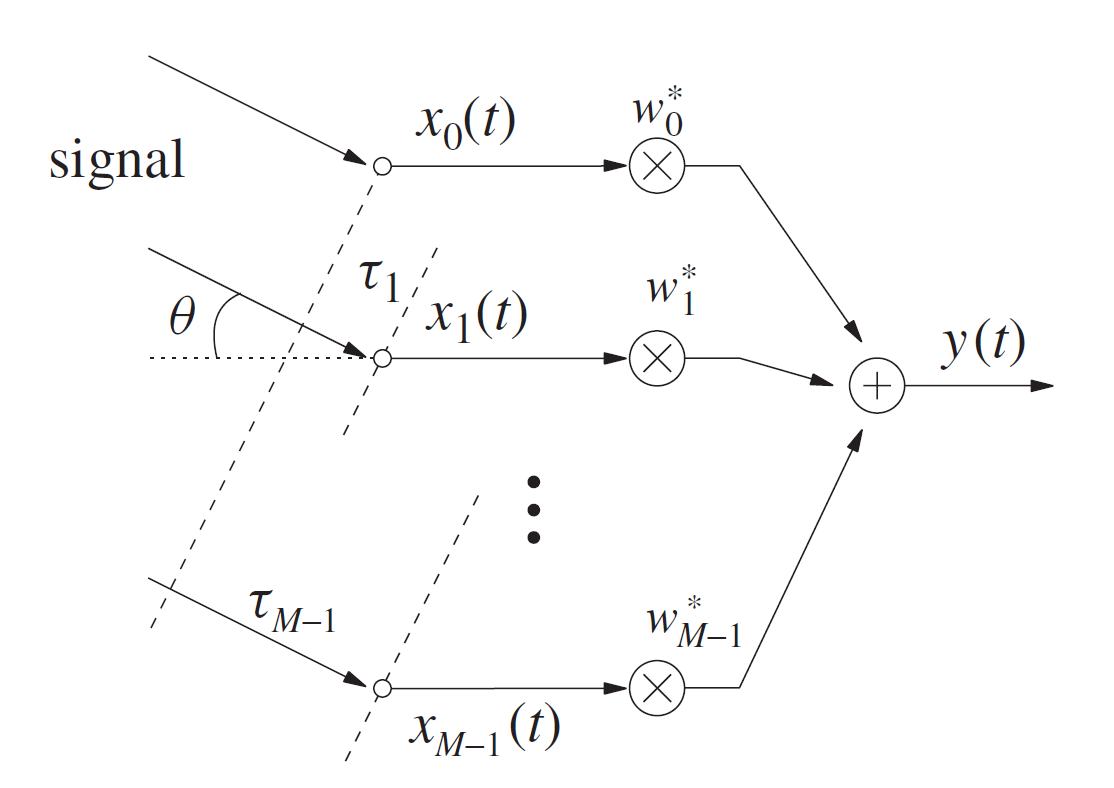
\includegraphics[scale = 0.7]{Figures/BF_RX_ULA.png}
    \caption[Combiner beamformer antenna array.]{Combiner beamformer antenna array. \cite{Liu2010}}
    \label{fig:combiner}
\end{figure}

The lapse in which one element receives the incoming signal to the following is given by the propagation speed of electromagnetic waves, the distance and the signal's direction of arrival, and is described by the equation \ref{eq:tau}, where $c$ is the speed of light. The consequence of this phenomena is that each antenna element in the array will get the same signal, but with a time delay ($\tau$) between adjacent elements. Each element's signal $x_{m}(t)$ is then multiplied by the complex conjugate of the constant $w_{m}$, which modifies the signal's amplitude and phase before adding them at the output stage. The mathematical model for ULA combiners is described by equation \ref{eq:combiner_time1}. \cite{Allen2005}

\begin{equation}
    \tau = \frac{d\:\sin(\theta)}{c}
    \label{eq:tau}
\end{equation}

\begin{equation}
    y(t) = \sum_{m=0}^{M-1}x_{m}(t)\:w_{m}^{*}
    \label{eq:combiner_time1}
\end{equation}

Assuming $x_{m}(t)$ is a complex wave, it can be replaced by its phasor form $x_{m}(t) = \exp(j\omega t)$. Hence, all the elements of the array can be replaced their phasor form and then add the lapse $\tau_{m} = m \tau$ as a phase shift. Also, the Direction of Arrival (DOA) $\theta$ is constrained to the range [$-\frac{\pi}{2}$,$\frac{\pi}{2}$], and the phase shift of the first element of the array is $\tau_{0} = 0$. The output of the combiner beamformer is given by equation \ref{eq:combiner_time2}, while its frequency response is given by equation \ref{eq:combiner_freq1}

\begin{equation}
    y(t, \theta) = \sum_{m=0}^{M-1} \exp(j \omega (t - \tau_{m}))\:w_{m}^{*} = \exp(j \omega t) \sum_{m=0}^{M-1} \exp(-j \omega \tau_{m})\:w_{m}^{*} = \exp(j \omega t) \sum_{m=0}^{M-1} \exp(-j \frac{\omega d \sin(\theta)}{c})\:w_{m}^{*}
    \label{eq:combiner_time2}
\end{equation}

\begin{equation}
    P(\omega, \theta) = \sum_{m=0}^{M-1} \exp(-j \omega \tau_{m})\:w_{m}^{*} =  \sum_{m=0}^{M-1} \exp(-j \frac{\omega d \sin(\theta)}{c})\:w_{m}^{*}
    \label{eq:combiner_freq1}
\end{equation}

Similar to digital signal processing, the antenna elements must be placed within a maximum distance from each other to avoid temporal aliasing. This constraint guarantees that the recovered signal by each antenna element to have a unique and ascending phase shift ($\angle{\exp(j\omega \tau_{m+1})} > \angle{\exp(j\omega t\tau_{m})}$). The signal's wavelength gives the constraint, and its described by the equation \ref{eq:distancing}. Replacing the constraint in equation \ref{eq:distancing} in equation \ref{eq:combiner_freq1} results in the frequency response for an optimal combiner. The beamformer's radiation pattern can be computed using equation \ref{eq:combiner_freq2}, which describes the array's magnitude at different directions of arrival.

\begin{equation}
    d \leq \frac{\lambda}{2} = \frac{\pi c}{\omega} = \frac{c}{2 f}
    \label{eq:distancing}
\end{equation}

\begin{equation}
    P(\theta) = \sum_{m=0}^{M-1} \exp(-j m \pi \sin(\theta)) w_{m}^{*}
    \label{eq:combiner_freq2}
\end{equation}

A beamformer's radiation pattern consists of two components: the main lobe and the side lobes. The main lobe is the most prominent and widest spike in the beamformer's magnitude; by default, the main lobe is centred at $0^\circ$. The side lobes are narrower and smaller lobes located near the main lobe, and these are often not desired. Finally, the area between lobes is called the null, as it has the lowest magnitude.

As previously stated, $w_{m}$ is a complex weight that describes the element's gain and phase shift. These parameters are used to steer the beamformer's main lobe and nulls to filter signals from the desired DOA deliberately and to attenuate signals from a different direction. Weights are also used to suppress the side lobes by using techniques as the ones used in DSP (FIR filter design and window functions). Each of the previous features is linked to a component of complex numbers; altering the magnitude may help reducing the side lobes while increasing the phase steers the main lobe. The complex weight is defined by equation \ref{eq:wn}, where $A_{m}$ is an array for suppressing the side lobes and $\phi$ is the desired steering angle. Replacing equation \ref{eq:wn} into equation \ref{eq:combiner_freq2} results in the frequency response of a optimal beamformer ($d = \lambda / 2$) with an steerable main lobe presented in equation \ref{eq:combiner_freq3}.

\begin{equation}
    w_{m} = A_{m} \exp(j m \pi \sin(\phi))
    \label{eq:wn}
\end{equation}

\begin{equation}
P(\theta, \phi) = \sum^{M-1}_{m=0} A_m \exp(-j m \pi (\sin(\theta) - \sin(\phi))) 
\label{eq:combiner_freq3}
\end{equation}

Steering the main beam may cause an undesired mirrored version of the same if the steering angle is above a certain value. This impairment is called Grafting lobe, and the steering angle range for avoiding it is given by equation \ref{eq:grafting}. The maximum steering angle for optimal beamformers (where $d = \lambda/2$) is $45^\circ$. Although this limitation can be solved by placing the antenna elements closer to each other, the array directivity is compromised, and more antenna elements are required to maintain the original gain pattern; resulting in a trade-off between maximum steering angle and directivity.

\begin{equation}
    \phi \leq \arcsin (\frac{\lambda}{d} - 1)
    \label{eq:grafting}
\end{equation}

\begin{figure}[!b]
    \centering
    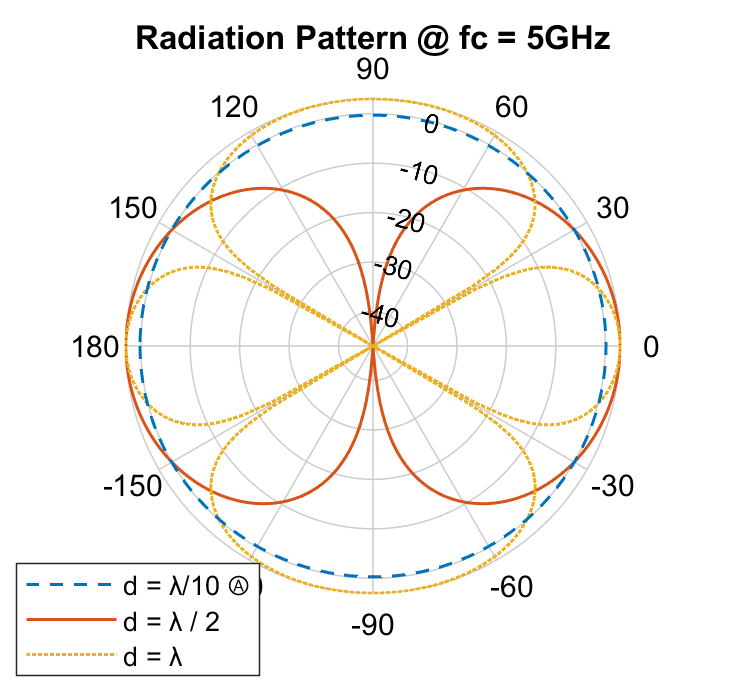
\includegraphics[width = 0.5\textwidth]{Figures/distance.png}
    \caption{Two-Element beamformer with different element distancing.}
    \label{fig:pattern_distance}
\end{figure}

Beamformers can be modelled as $(M-1)^{th}$ order band-pass FIR filter. The filter's normalised pass-band and stop-band frequencies can be input as the main lobe's pass-band direction and stop-band direction. This property makes designing weights for sidelobe suppression simple using tools like MATLAB. The only concern the designer needs to consider is that beamformers have the same limitations as FIR filters and sharp responses require arrays with many elements \cite{Liu2010}. If the designer does not desire to implement side lobe suppression, then $A_m$ may be defined as a unitary array.

\subsection{Implementing Beamforming} \label{back:bf:impl}
Although Beamforming's only requirement is to satisfy the equation \ref{eq:combiner_freq3}, real implementation of beamformers is usually categorised into three types. The main difference between the three types is where the precoder and combining stages are performed.

\subsubsection{Analogue Beamforming} \label{back:bf:impl:abf}
Analogue Beamforming performs precoding and combining using specialised circuitry hardware; this makes an exceedingly power-efficient and cost-effective beamformer; since the incoming or transmitted signals can be processed without even considering Beamforming is applied in the system, excluding the steering algorithm.

It also saves on the use of RF Front Ends, since one of these can drive multiple antennas while keeping a hardware phase shifter and amplifier to each antenna. Having this is much better in terms of power and cost-efficiency.

The disadvantage of Analogue Beamforming is the reduced flexibility and added hardware complexity, which also makes steering the main lobe more difficult.

\subsubsection{Digital Beamforming} \label{back:bd:impl:dbf}
Digital Beamforming main feature is the ability of precoding or combining using DSP algorithms; making this type of beamformer very flexible and configurable by only modifying the DSP algorithm in a processor.

It is also the simplest one to implement using off-the-shelf components since each antenna requires much hardware to receive or transmit signals. This detail makes Beamforming possible using existing solutions or Software Defined Radio units.

The most significant disadvantages of Digital Beamforming is the low scalability efficiency, due to the cost and power requirements of having an RF Front End to drive a single antenna.

\subsubsection{Hybrid Beamforming} \label{back:bf:impl:hbf}
This implementation combines the attributes of both Analogue and Digital Beamforming by allowing the system to perform the precoding and combining in both baseband and broadband domains. 

This type of beamformer combines the benefits and only a few disadvantages of both Analog and Digital Beamforming, by having flexibility and power and cost-efficiency. This benefit allows Hybrid Beamforming to be implemented on a large scale.

Some disadvantages of Hybrid Beamforming are the increased hardware and software complexity to be able to perform combining and precoding efficiently in both domains.

\subsection{Adaptive Beamforming} \label{back:bf:adapt}
Adaptive Beamforming is a technique to update the beamformer's weight according to the incoming signal; mostly to detect the direction of the incoming signal and steer the main lobe accordingly, while suppressing interference. Adaptive Beamforming is only a category of a total of three; other techniques such as scanning and switched Beamforming are mature technologies, but the most flexible and efficient beamformers are adaptive.

\subsubsection{The Spatial Covariance Matrix} \label{back:bf:adapt:scm}
Most of the adaptive beamformers require to compute channel estimation techniques, but instead of using pilots, they use something called the Spatial Co-variance Matrix. This matrix, often referred to as the $R_{u}$, matrix,  while its subscript represents the device that computes the matrix; in this case, the Uplink (The User Equipment). The Spatial Covariance Matrix is given by the Expected Value ($E[X] = \int_{0}^{\infty}xf(x)$) of the auto-correlation of the received signal \cite{Allen2005}.

\begin{equation}
    \label{adpt:scm}
    R_{u} = E[uu^{H}]
\end{equation}

\subsubsection{Temporal Reference Algorithms} \label{back:bf:adapt:tr}
Many algorithms are based on the Wiener Solution, which consists in optimising the error signal $J = E[|e(k)^{2}|]$ to obtain the optimised weights $W_{opt}=R_{u}^{-1}P_{u}$, where $R_{u}$ is the spatial correlation matrix and $P_{u}$ is the cross-correlation between the input and desired signals. The computational requirement of this algorithm is significant since a matrix must be inverted. Because of this, other algorithms such as the Method of Steepest Descent, Least Mean-Squares, Direct Matrix Inversion and Recursive Least-Squares are used to lower the computational requirement by using estimations and recursive solutions. \cite{Allen2005}

\subsubsection{Source Location Algorithms} \label{back:bf:adapt:sl}
Other algorithms called Source Location Techniques, these allow the UE to find the direction of the base station and then to update the steering angle ($\phi$) while keeping the previously designed weights. Two of the most popular methods are the MUSIC and ESPRIT algorithms. Is fair to say that these algorithms do not directly output the estimated DOA; instead, they return the spatial spectrum, and the peaks of this spectrum are interpreted as the DOA. \cite{Allen2005}

%The way Source Location algorithms can estimate the DOA is by applying an "inverse" operation to beamforming that considers a $F$ amount of source signals $S(t)$ arriving at a ULA. The MUSIC algorithm can track the source direction of both $S(t)$ signals by estimating the covariance matrix of the received signal $R_u$ and computing a pseudo space spectrum based on the orthogonality of the 

\newpage
\section{Software-Defined Radio} \label{back:sdr}
\subsection{Introduction} \label{back:sdr:intro}
Software Defined Radio (SDR) is a term to refer to radio systems with almost all its functionality done in software, instead of hardware as it is commonly found in most of the RF applications in recent times. An ideal SDR, as shown in Figure \ref{fig:SDR_Ideal}, would have an RF Front End only consisting of a power amplifier and high-speed Analogue to Digital converter. Hence, the remaining physical layer functions such as modulation, synchronisation or encoding are done using DSP. \cite{Stewart}

SDR systems are expected to work in a wide range of the frequency spectrum and to perform various operations as a dedicated hardware implementation would have. For example, using a low-cost SDR unit for hearing a local FM radio station and for getting an OFDM signal using QAM modulation in the 2.4 GHz band are both widespread uses.

\begin{figure}[h]
    \centering
    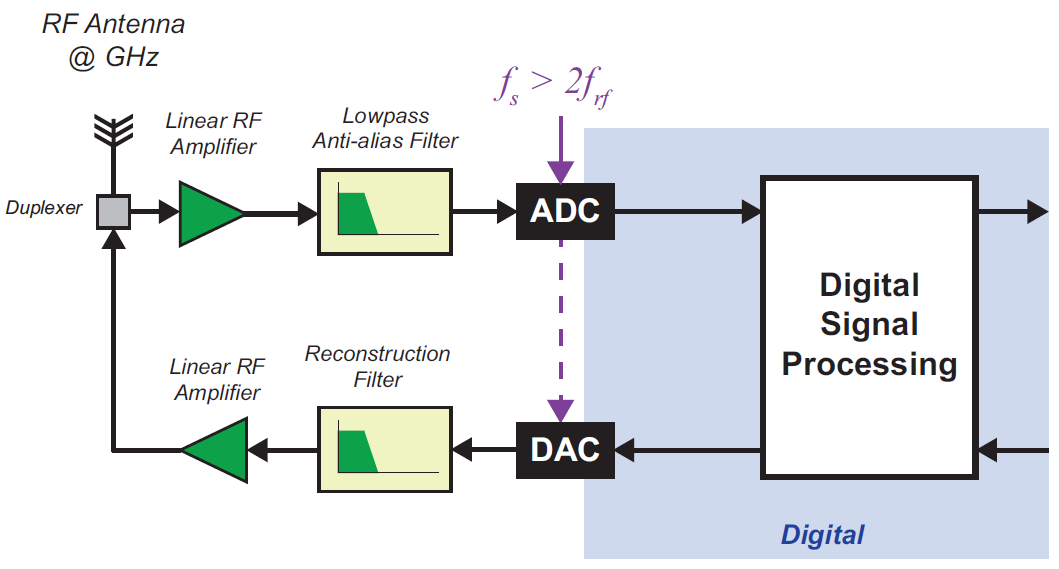
\includegraphics[scale=0.7]{Figures/SDR_Ideal.png}
    \caption[Ideal SDR block diagram.]{Ideal SDR block diagram. \cite{Stewart}}
    \label{fig:SDR_Ideal}
\end{figure}

\subsection{Hardware and Flexibility} \label{back:sdr:hdwr}
\subsubsection{Model-Based Design and Hardware in the Loop} \label{back:sdr:hdwr:mbd}
Unlike old radio units using specialised hardware to receive and process a particular kind of incoming signal, SDR hardware is generic enough to process data of several frequencies and modulation schemes; a Field Programmable Gate Arrays (FPGA) inside the SDR radio often does this feature. FPGAs in the context of DSP, are faster and more efficient than microcontrollers; because of the dedicated DSP slices inside the silicon, the higher processing speed for RF applications and the available tools to design and simulate RF systems.

High-Level Synthesize (HLS) systems like MATLAB/Simulink, Python or SystemC are used to model an RF system, simulate it to properly tuning and debugging, and finally generating HDL code to program the real hardware according to the model. This process is called Model-Based design. HLS software may already have specific tools to implement specific hardware or software processes, making the model generation even more comfortable. 

Another commonly used design methodology is the Hardware in the Loop (HIL). Similar to Model-Based Design, HIL uses a high-level modelling software such as MATLAB/Simulink or GNU Radio to develop an algorithm of the system which includes the SDR as part of the model. Often, HIL limits the capability of the SDR as no custom HDL is generated to be executed in the FPGA; this method uses the SDR as a signal source and sinks so the computer can execute the intended algorithm. HIL models are faster to test and verify than Model-Based Design and also easier to create as no subsystems are compiled into HDL; however, a performance penalty is present as the algorithm is not being wholly executed in hardware.

\subsubsection{Transceiver Architectures} \label{back:sdr:hdwr:arch}
An essential stage in SDRs is the AD/DA conversion architecture. There are three different architectures to get or produce signals. The Heterodyne architecture is the oldest from the three, and consists of a physical downconverter using a mixer and a local oscillator (LO); this method shifts the received broadband signal to baseband for the  ADC to sample it, or in the opposite direction if a DAC is generating the signal. The Direct Conversion architecture (Also known as Zero-IF), doubles the bandwidth efficiency by adding a second Heterodyne converter, but the LO signal for the second converter is shifted by $90^\circ$; this enables having two independent data streams known as the In-Phase and Quadrature (IQ) signals. Finally, the Direct Sampling architecture converts signals from broadband to baseband and vice versa using software; this is the most demanding method as the DAC/ADC must have a sampling rate in the order of hundreds or even thousands of MHz. However, this method offers the most excellent flexibility as the signal can be easily modified even when it is up-converted. 

\begin{figure}[h]
\centering
    \begin{subfigure}{0.45\textwidth}
        \centering
        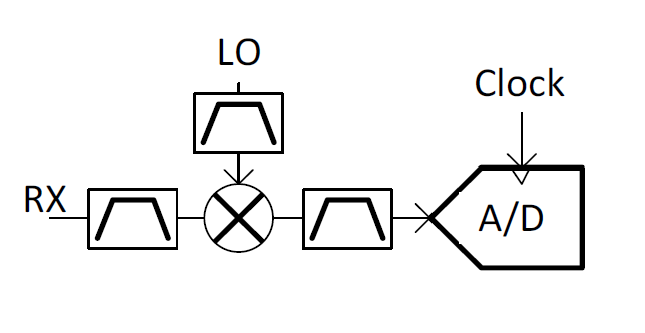
\includegraphics[scale = 1.1]{Figures/SDR_HET.png}
        \caption{Heterodyne receiver}
    \end{subfigure}
    \begin{subfigure}{0.45\textwidth}
        \centering
        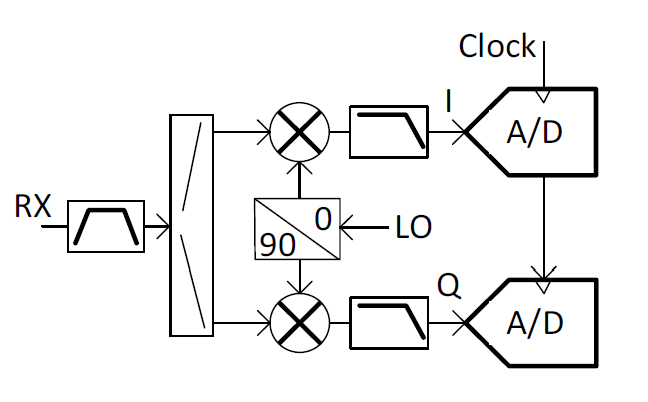
\includegraphics[scale = 1]{Figures/SDR_ZIF.png}
        \caption{Direct conversion receiver}
    \end{subfigure}
    \newline
    \begin{subfigure}{\textwidth}
        \centering
        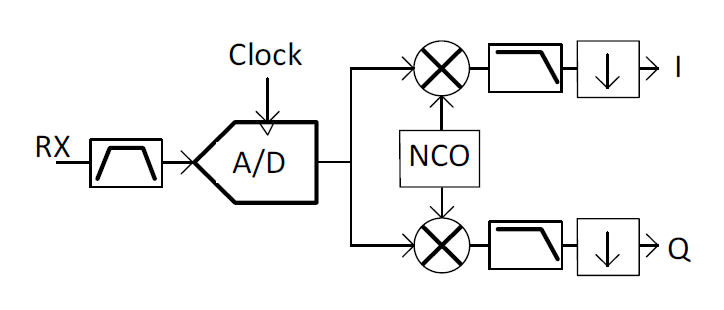
\includegraphics[scale = 1]{Figures/SDR_DS.png}
        \caption{Direct sampling receiver}
    \end{subfigure}
    \caption[Receiver architectures.]{Receiver Architectures. \cite{ad9361}}
    \label{fig:receiver_architectures}
\end{figure}

Most of the SDRs in the market use the Direct conversion architecture, as it is compatible with many kinds of signals such as AM, FM, PSK and QAM. Additionally, most SDRs use RF front-ends packed in a single IC, providing a power amplifier, mixer, RF filter, ADC/DAC and data interface for it to be used with many microcontrollers. Many of these ICs also include several coherent TX and RX channels using a single LO. Two important manufacturers of transceiver ICs are Lime Microsystems and Analog Devices.

\begin{figure}[h]
    \centering
    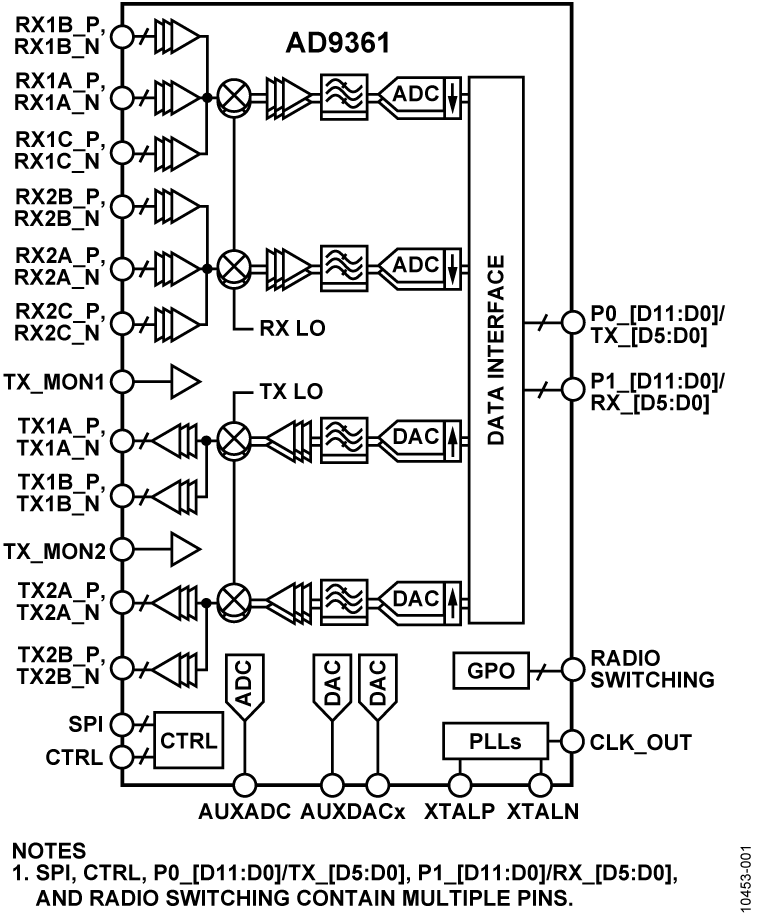
\includegraphics[scale = 0.3]{Figures/AD9361.png}
    \caption[AD9361 RF Transceiver block diagram.]{Block diagram of the AD9361 RF transceiver. \cite{ad9361}}
    \label{fig:ad9361}
\end{figure}

\subsection{Available Software-Defined Radio Units} \label{back:sdr:avail}
Many SDR units are available to buy today, the vast majority of them are meant for research and industrial applications with companies such as Ettus Research and National Instruments being two of the most popular SDR manufacturers. These devices are expected to have many features such as full-duplexing, high-performance FPGAs, wide frequency range (Even supporting the mm-Wave), wide baseband bandwidth, MIMO or compatibility with existing development tools.

Other SDR units are intended to be used by students, makers or even engineers; basically, everyone who is budget is not large enough to get a device from the previously mentioned manufacturers. Platforms such as the RTL-SDR, LimeSDR, HackRF, BladeRF and PlutoSDR are examples of devices that target this budget range. These devices are examples of open-source projects (Excepting the Pluto SDR) maintained by the community, some with modest capabilities and compatibility. Meanwhile, companies like Analog Devices back the design and production of their Pluto SDR, which is intended for students to learn digital communication systems. 

\begin{table}
\centering
\begin{tabular}{c|c|c|c|c|c|c}
SDR & Ettus B210 & Hack RF & RTL-SDR & LimeSDR & PlutoSDR & BladeRF 2 \\ 
\hline 
Max Freq & 6 GHz & 6 GHz & 1.7 GHz & 3.8 GHz & 3.8 GHz & 6 GHz \\ 
RF Bandwidth & 61.44 MHz & 20 MHz & 2.4 MHz & 61.44 MHz & 20 MHz & 61.44 MHz \\ 
Interfacing & USB3.0 & USB2.0 & USB 2.0 & USB3.0 & USB 2.0 & USB3.0 \\
Sample Depth & 12-bit & 8-bit & 8-bit & 12-bit & 12-bit & 12-bit \\ 
Duplex & Full & Half & N/A & Full & Full & Full \\ 
MIMO & 2x2 & 1x1 & 0x1 & 2x2 & 1x1 & 2x2 \\ 
TX Power & 10 dBm & 15 dBm & N/A & 10 dBm & 7 dBm & 8 dBm \\ 
%Price (USD) & \$1119 & \$299 & ~\$10 & \$299 & \$149 & \$480\\ 
\end{tabular}
\caption[SDR comparison table.]{SDR comparison table \cite{sdrtable, RTL-SDR.com2020RTL-SDRDatasheet, Nuand2018BladeRFMicro}}
\label{tb:SDRcomp}
\end{table}

\newpage
\section{Beamforming in Software-Defined Radio} \label{back:bf_sdr}
Since the essential requirements of Beamforming mostly rely on the placing of the antenna array and not so much on signal processing, it is suitable to be implemented in SDR systems. Of-the-shelf SDR devices already have the required hardware to drive multiple antennas, making of Digital Beamforming the most convenient of the three alternatives. Implementation as in \cite{Gaydos2018, Nayeri2016} used specialised hardware in order to set up the multiple SDR units quickly, and LabVIEW was used as the interface to control and monitor the antenna array; showing the capabilities of high-end SDR equipment. Low-cost SDRs are not as flexible as the previously mentioned as additional effort, knowledge and sometimes hardware modifications are required to do a similar implementation as \cite{Gaydos2018, Nayeri2016} in these devices.

Many non-ideal conditions can result in beamformers showing erratic behaviour or can even break them. Impairments such as correlation error, mixer frequency shifts or non-synchronised oscillators among others must be considered when designing a Digital Beamformer \cite{Delos2017}. Fortunately, SDR manufacturers have already solved most of the previously mentioned impairments; however, the most critical impairment to consider when using SDR based beamformers is related to synchronisation.

\subsection{Coherence and Synchronisation} \label{back:bf_sdr:sync}
According to \cite{Delos2017, AD2017}, Digital beamforming requires both transmitter and receiver to be coherent or pseudo-coherent; this implies that the phase between channels must be consistent, zero for pure coherent systems or constant for pseudo-coherent. Also, the sampling clock of the ADC/DAC must be perfectly aligned between channels. Distributing a LO signal to every SDR or RF front-end is the easiest way to synchronise the relative phase of each properly, but noise in the distributed signal can significantly affect the performance of the beamformer. An alternative to this is to keep each SDR LO and distribute a low-frequency trigger signal that keeps every LO aligned without having a noiseless signal source.

\subsection{Interfacing} \label{back:bf_sdr:int}
Transfer speed is an important parameter to consider, as receiving data from multiple antennas does increase the required interfacing bandwidth from the SDR to the processor in a factor of the number of antennas; for example, having a four-element antenna array each one sampled at 10 MSPS transferring the IQ samples as a 32-bit integer type results in the following required throughput.

\begin{equation*}
    R_{req} = (4 \: \text{antennas}) (32 \frac{\text{bits}}{\text{sample}}) (10E6 \: \frac{\text{samples}}{\text{second} \times \text{antenna}}) = 1.28 \: \text{Gbps}
\end{equation*}

The past example requires a total of 1.28 Gbps, which is much higher than the maximum theoretical speed of USB2.0 (480 Mbps), meaning that a faster protocol is required such as USB3.0 (5 Gbps - 20 Gbps) or Ethernet (1 Mbps - 400 Gbps) \cite{USB2, USB3, Ethernet}. On top of that, the real throughput of these protocols dramatically depends on the frame size. However, designers can choose the sample rate, and SDRs have different bit-depths, so the required throughput differs from one device to another.

\subsection{Transceiver Architecture} \label{back:bf_sdr:type}
As previously stated, SDRs implement external transceiver ICs that use the Direct-Conversion architecture as shown in figure \ref{fig:receiver_architectures}, meaning that signal can only be processed in baseband. This design decision constrains the beamforming type to Phase-shift Beamforming, in which the time-delays shown in equations \ref{eq:combiner_time2} and \ref{eq:combiner_time3} are treated as phase shifts in the IQ signals. However, Phase-Shift Beamforming introduces the maximum steering angle, as shown in equation \ref{eq:grafting} and non-ideal radiation patterns. This limitation is caused by the phase coherence in the TX or RX channel, as the real beamforming equations consider a time-delay between the carrier signals and the resulting signal is shown in equation \ref{eq:phase_shift_bf}. \cite{Jang2018ABeamformer}

\begin{equation}
    y_m(t) = I(t-\tau_m) \cos(\omega t) - Q(t-\tau_m) \sin(\omega t)
    \label{eq:phase_shift_bf}
\end{equation}

\begin{equation}
    y_m(t) = I(t-\tau_m) \cos(\omega (t - \tau_m) - Q(t-\tau_m) \sin(\omega (t - \tau_m))
    \label{eq:true_time_delay_bf}
\end{equation}

More flexible architectures as the Direct Sampling in figure allows True Time-Delay Beamforming, which allows the signal to be modified even in broadband resulting in a transmitted or received signal similar to equation \ref{eq:true_time_delay_bf}, removing the steering angle constrain of $45^\circ$ before getting grafting lobes, assuming an optimal beamformer. As this beamforming type seems to be more effective than Phase-Shift Beamforming, it requires a shallow sampling rate in the order of picoseconds, which is unobtainable for low-cost ADC/DAC. 


\chapter{Methodology} \label{met}
\section{Introduction} \label{met:intro}
This chapter describes the work done to accomplish the objectives in section \ref{intro:obj}. The work done for this project is divided into several disciplines, being these listed as follows.

\begin{itemize}
    \item Simulation
    \item SDR selection
    \item MATLAB interface for SDR
    \item Antenna mounting
    \item HIL Demo
\end{itemize}

The previous bullets are not in chronological order as several stages were being developed simultaneously, but the result of this section is a demonstration to show the test bench capabilities.

The end result of this section is a Hardware-in-the-Loop Simulink model that interfaces the algorithms used in the simulation model described in section \ref{met:sim}, using the MIMO interface for the SDR shown in section \ref{met:int} and an antenna holder for fulfilling the spatial sampling requirement of beamforming, shown in section \ref{met:mount}. The resulting HIL model is shown in section \ref{met:hil}.

The Simulink models, the MATLAB MIMO interface for the SDR and other scripts are available in the repository shown in Appendix \ref{appendix}.

\newpage
\section{Simulation} \label{met:sim}
A simulation model of an downlink end-to-end communication system was made to test the beamforming algorithm in both transmitter and receiver sides. As the objective of this section is to deliver a usable beamforming model supporting both TX and RX arrays, the HIL approach is appealing, as the subsystems of the simulation can be reused in the HIL model with a few modifications. This simulation was done using Simulink since it supports many algorithms and models commonly used in digital communications and also supports HIL workflows with many SDRs.

Many iterations of the end-to-end simulation were created, including more features and with real-life impairments and characteristics. The simulation and its subsystems were developed simultaneously and then tested in different models, as described in chapter \ref{test}. The final iteration of the simulation model includes the following subsystems. The resulting model is shown in figure \ref{fig:sim}.

\begin{multicols}{2}
\begin{itemize}
    \item User equipment's movement pattern
    \item Modulator at the base station
    \item Receiver at the user equipment
    \item TX beamformer at the base station
    \item RX beamformer at the user equipment
    \item Wireless channel
\end{itemize}
\end{multicols}

Similar to the subsystems, a setup MATLAB script was created to manage the block's parameters in the system and to automate changes to many parameters. The script will be described as the equations related to each subsystem. Since the model only represents the downlink scenario, the BS Modulator subsystem will be referred as the Modulator, and the UE Receiver subsystem as the Receiver, as only one of each is present in the model.

Simulation results are available in chapter \ref{test} as the model described in this section is generic and many parameters depend on the selected SDR.

\begin{figure}[h]
    \centering
    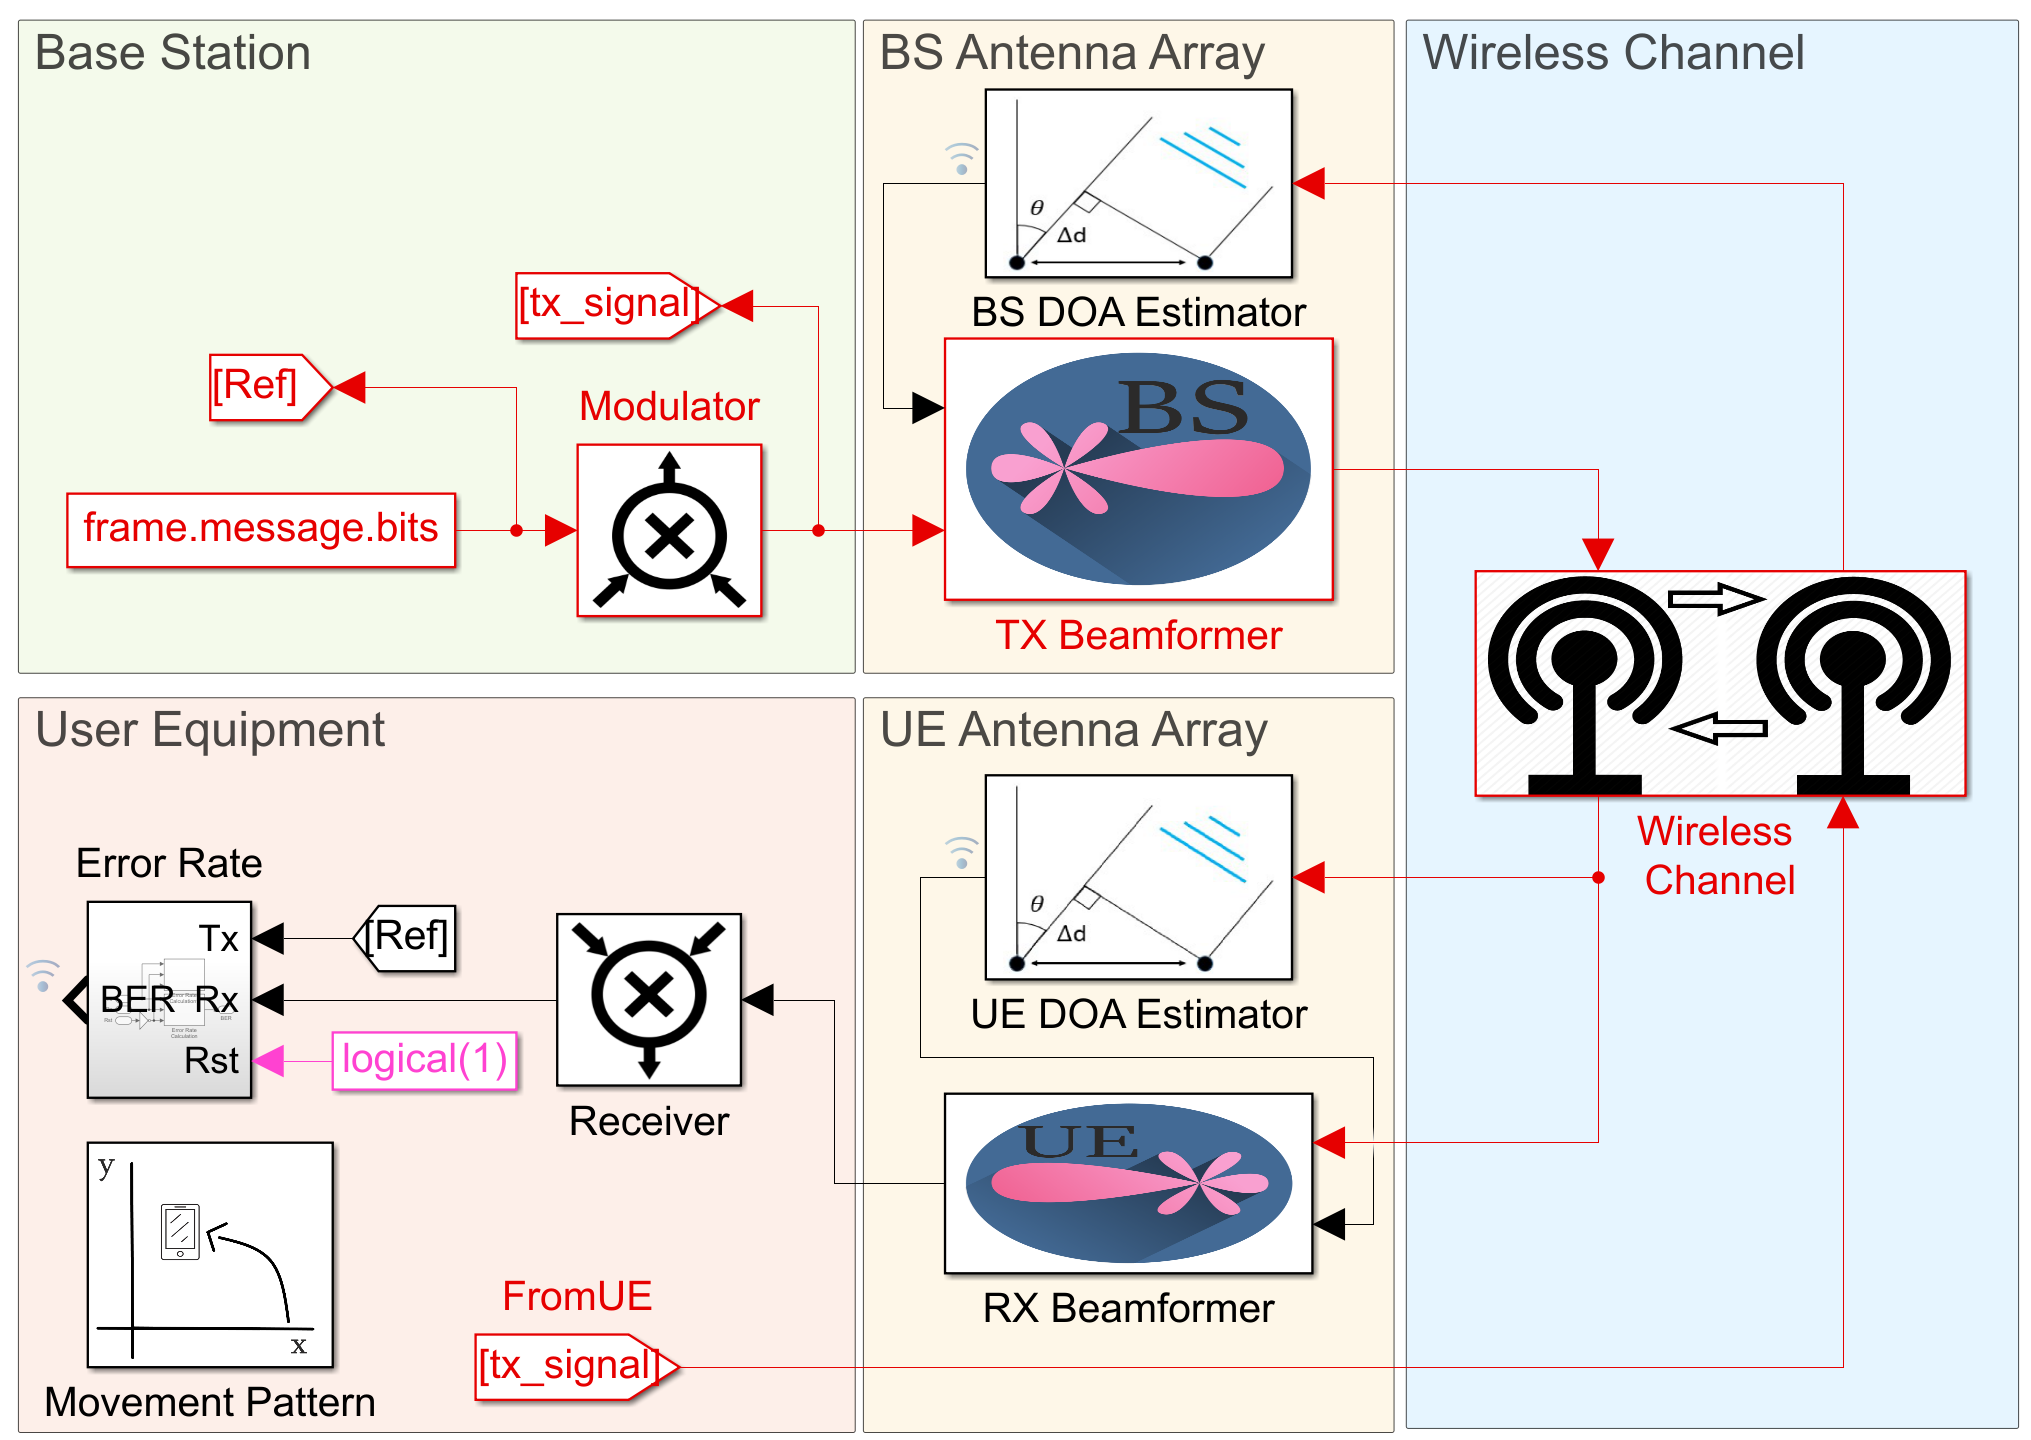
\includegraphics[width = 0.8\textwidth]{Figures/sim_model.png}
    \caption{Simulink model for the UE tracking simulation.}
    \label{fig:sim}
\end{figure}

\subsection{Problem Statement and Initial Assumptions} \label{met:problem}
The simulation model assumes two devices are located in space, the base station (BS) and the User Equipment. The BS is located at the origin of a coordinate system and is unable to move in any direction. The UE is located at a distance $\due$ and is allowed to rotate around the BS. The UE is oriented in a constant direction $\Azue$, which represents the azimuth angle of the UE (absolute orientation, relative to the coordinate system). Finally, the elevation angles at both the UE and BS are discarded.

The BS consists of two M-element antenna arrays for both TX and RX stages and a processing unit. The UE has a single M-element RX antenna array, single antenna TX stage and a processing unit. All the antenna arrays in the model are assumed to be optimal ULAs composed of isotropic antennas.

The goal of this system is for the BS to track and lock the UE using both of its antenna arrays in order to maintain a constant Bit Error Rate in the end-to-end communications system. Besides, the UE can use beamforming at the receiver end to enhance the Signal-to-Noise (SNR).

The challenge for both devices is to locate each other's direction using their transmitted signals. This model assumes that all the antenna arrays are placed along the $y$ axis; antenna elements overlap in the case of the BS, as it has two arrays. The UE's location relative to the BS will be called the Direction of Departure (DOD), as it is the angle at which the BS must steer the TX beam to reach the UE. Similarly, the BS's location relative to the UE's orientation will be called the Direction of Arrival (DOA), as it is the orientation at which the UE must steer its RX beam to capture the BS's signal optimally. Both angles are measured from the positive $x$ axis to the positive $y$ axis.

The UE's position relative to the BS is an arbitrary function of time. The sinusoid gives the rotation function in equation \ref{eq:DOD} where $DOD_{max}$ is the maximum angle of departure, and $f_{UE}$ is the frequency of the sinusoid; both of these are input parameters. As this simulation is a discrete system, it must account a sampling time $T_{s}$ and a sample number $n$. The DOA can be easily derived by adding the UE's azimuth to the DOA. The constraint in equation \ref{eq:DOD} restricts the DOA to a range of $\pm 90^\circ$; as this is the input range of the blocks in the following sections. 

\begin{equation}
    DOD(n) = DOD_{max} \sin(2 \pi n T_{s} f_{UE}), \:|DOD_{max} + \Azue| < 90
    \label{eq:DOD}
\end{equation}

\begin{equation}
    DOA(n) = DOD(n) + \Azue
    \label{eq:DOA}
\end{equation}

Figure \ref{fig:sl:movement}, shows the Simulink model for the system kinematics. The Sine Wave and subtraction blocks represent equations \ref{eq:DOD} and \ref{eq:DOA}, and there also is a manual switch for keeping a constant DOD. Also, a visual representation of the simulated environment is shown in figure \ref{fig:coordinate_examples}.


\begin{figure}[h]
\begin{subfigure}{0.5\textwidth}
    \centering
    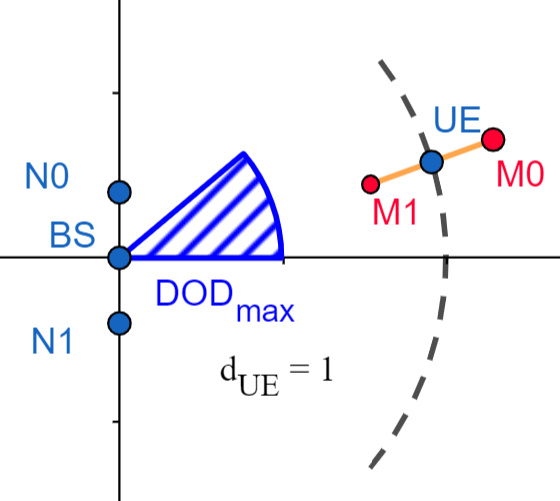
\includegraphics[width = 0.6\textwidth]{Figures/simulation_environment.png}
    \caption{Parameter visualisation.}
    \label{fig:coordinte}
\end{subfigure}
\begin{subfigure}{0.5\textwidth}
    \centering
    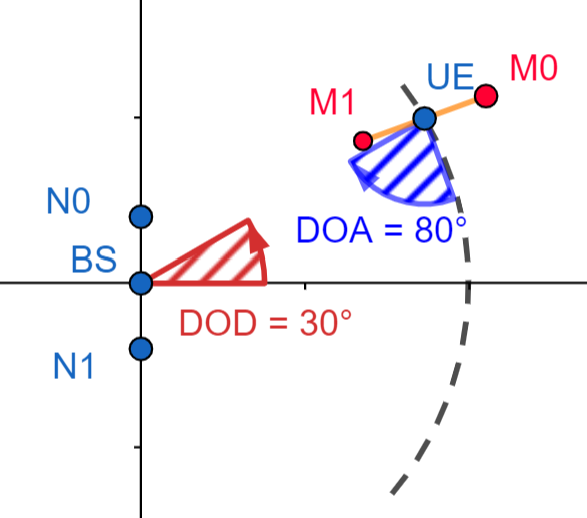
\includegraphics[width = 0.6\textwidth]{Figures/simulation_environment_angles.png}
    \caption{DOD/DOA visualisation.}
    \label{fig:angles}
\end{subfigure}
\caption[Example of the coordinate system.]{Example of the coordinate system assuming $\due = 1$, $\Azue = 20^\circ$ and $M = 2$. Points M0 and M1 are the antenna array.}
\label{fig:coordinate_examples}
\end{figure}

\begin{figure}[!h]
    \centering
    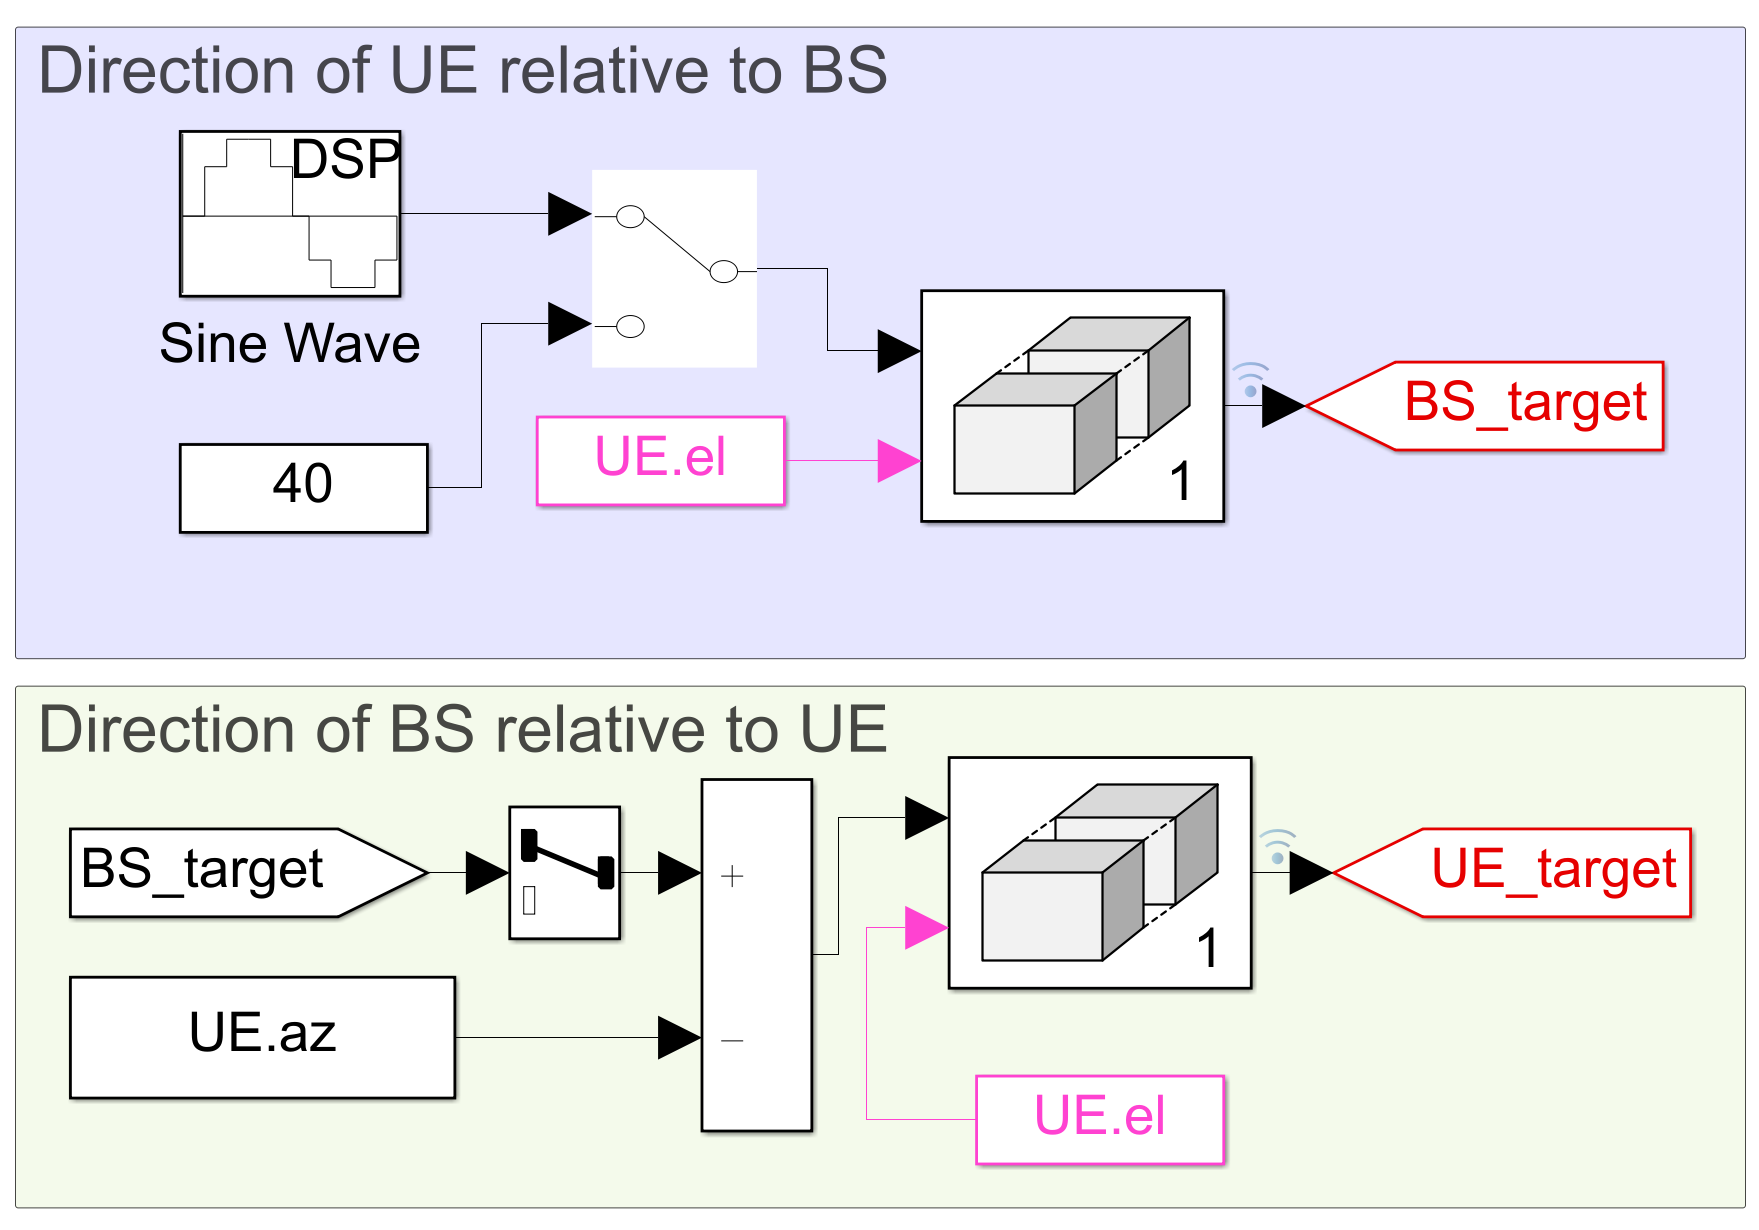
\includegraphics[width = 0.6\textwidth]{Figures/SL_movement.png}
    \caption[Simulink subsystem for the UE's movement.]{Simulink subsystem for the UE's movement, part of the model in figure \ref{fig:sim}.}
    \label{fig:sl:movement}
\end{figure}

\subsection{Modulator and Receiver} \label{met:sim:mod}
The purpose of this section is to define the parameters and techniques used in the wireless communication system that were used around the beamforming algorithm. As this simulation will later involve actual hardware in it, the subsystems must consider that SDRs are discrete systems that operate using frames with many symbols per iteration. Similar to the derivation of equation \ref{eq:DOD}, the simulation model requires a fixed time step $T_{s}$ in which the modulator and receiver algorithms are executed. Both Modulator and Receiver algorithms are standard procedures commonly used in communication systems, and these particular subsystems are based on the examples provided by MATLAB and Simulink in \cite{Mathworks2020QPSKKingdom}.

\subsubsection{Modulator} \label{met:sim:mod:mod}
The simulation is supposed to transmit a frame of $N_M$ message bits; this sequence remains constant through the simulation time. This sequence is meant to be processed and modulated so the receiver algorithm can output the same message sequence. This task is done in the Modulator subsystem, which performs the following actions: Scramble, add preamble, modulate and interpolate. These actions are done in the same order as listed.

The scrambler is used to mix the message bit in case these are many consecutive appearances of a bit pattern, particularly helping the Automatic Gain Controller stage at the receiver. The preamble is a constant bit sequence that helps the receiver know where a frame starts; the length of the sequence $N_P$ is essential as the larger it is, the easier it is to detect it, at the expense of occupying more space in the sent frame. After both scrambled message and preamble sequences are added together, the resulting sequence is then modulated using QPSK, outputting a new sequence of $N_S$ complex symbols.

\begin{equation}
    N_S = \frac{N_M + N_P}{2}
    \label{eq:nsym}
\end{equation}

The last step in the modulator block is interpolating the symbol sequence. This step is vital as the SDR introduces a baseband sampling rate ($f_{bb}$), which in many units has a relatively high minimum value. The up-scaling is done using a Raised Cosine (RC) filter, which also reduces the Inter-Symbol-Interference. The RC filter can interpolate the symbol sequence to satisfy any sample rate while reducing ISI by slightly increasing the signal's bandwidth using the RC's roll-off factor ($\beta$). The interpolation factor ($N_{int}$) is given by equation \ref{eq:inter}, which uses the simulation's symbols per time step ($N_{s/s}$); also, the RC filter is an IIR filter, its span must be limited.

The modulator algorithm is coded into Simulink, as shown in figure \ref{fig:sl:modulator}.

\begin{equation}
    N_{s/s} = T_s f_{bb}
    \label{eq:sym_per_step}
\end{equation}

\begin{equation}
    N_{int} = \frac{N_{s/s}}{N_S}
    \label{eq:inter}
\end{equation}

\begin{figure}[h]
    \centering
    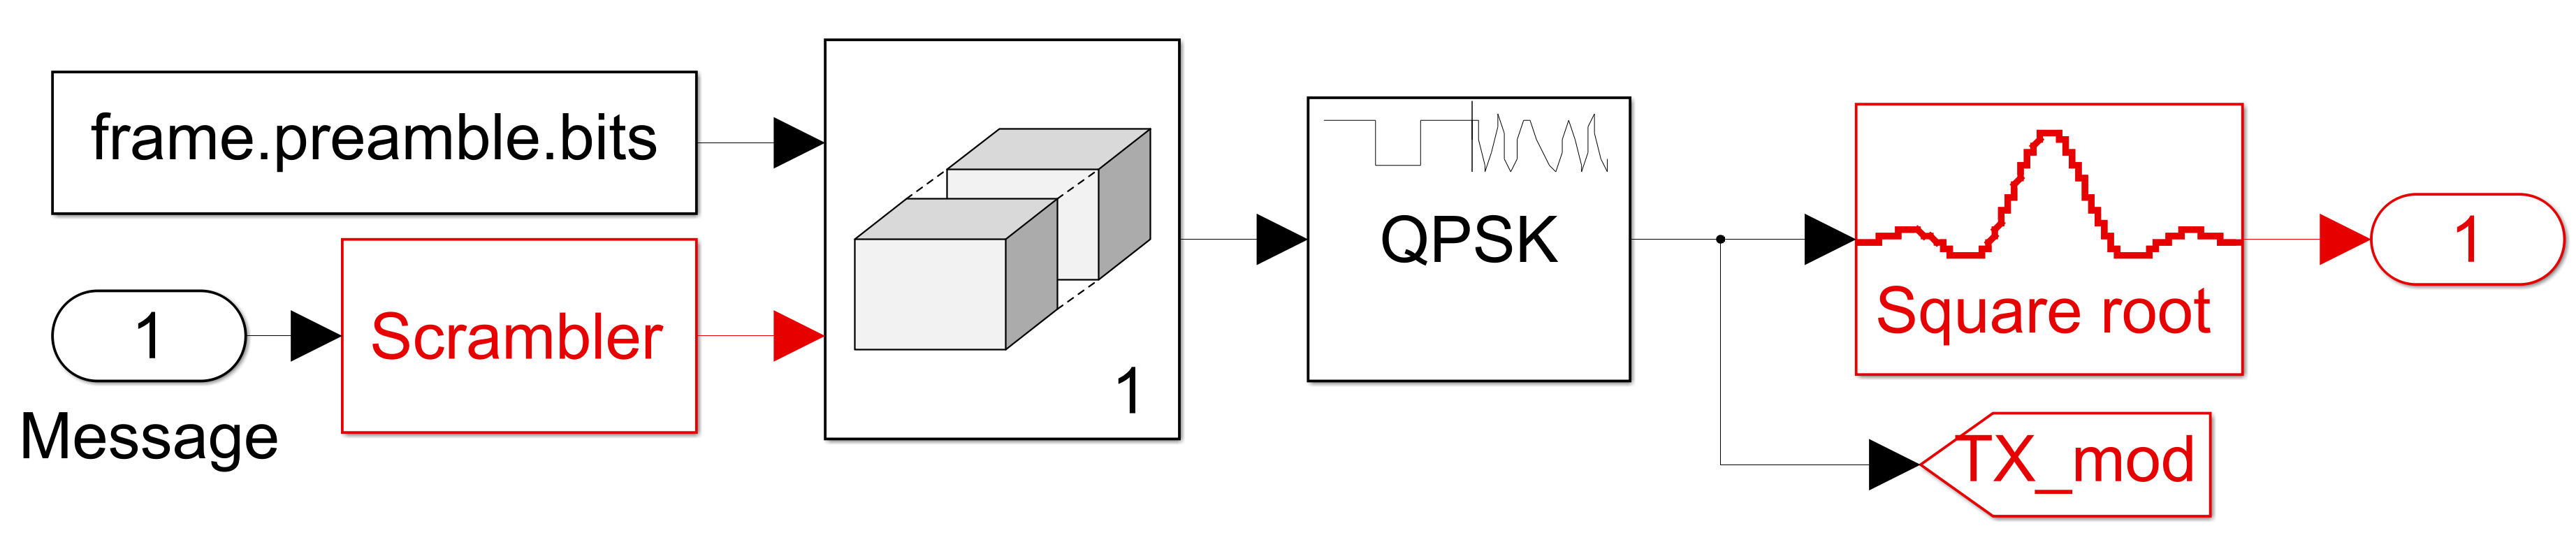
\includegraphics[width = 0.8\textwidth]{Figures/SL_modulator.png}
    \caption[Simulink subsystem for the Modulator]{Simulink subsystem for the Modulator, part of the model in figure \ref{fig:sim}.}
    \label{fig:sl:modulator}
\end{figure}

\subsubsection{Receiver} \label{met:sim:mod:rec}
The receiver part includes the counter-operation of every step of the modulator and some other stages to consider the channel and timing impairments properly. This block's task is to output the message bits that were the input of the Modulator block. The stages are executed as follows: Decimation, normalisation, carrier synchronisation, symbol synchronisation, frame synchronisation, phase correction, preamble removal, de-modulation and de-scrambling.

Similar to the modulator, the Raised Cosine filter improves ISI while decimating the received signal; the only difference in this stage is that the decimation factor $N_{dec}$ must be smaller than the interpolation factor ($N_{dec} < N_{int}$) as the following stages require an input signal with many samples per symbol. The Automatic Gain Controller (AGC) normalises the signal's amplitude, usually for its IQ component's maximum value to be unitary; AGC uses an open-loop approach that averages a sampling window, and it may not act in every simulation step, as the signal is not expected to change its amplitude very abruptly. The AGC helps the Preamble Detector to output a repeatable result as it is greatly affected by the signal's power. The carrier synchronisation step corrects the frequency and phase impairment introduced by the LOs at the TX and RX ends. This stage may introduce some errors as it has a transient state in which it tries to compensate for the signal's phase error. The output of this block should roughly match the output of the Modulator block, but a phase error could still be present; the magnitude of the phase error depends on the modulation scheme; QPSK phase error is described in equation \ref{eq:qpsk_phase_error}. 

\begin{equation}
   \alpha_{error} = k \frac{\pi}{4}, k = 0, 1, 2, 3
   \label{eq:qpsk_phase_error}
\end{equation}

The symbol synchroniser stage uses the up-sampled signal to get a down-scaled symbol sequence that contains the sent frame. Then, the frame synchroniser stage outputs the frame by using a preamble detector. The detector uses the magnitude of the cross-correlation function to get the position of the frame after the symbol synchronisation;  then, it is fed to the frame synchroniser. Using the cross-correlation approach also discards the remaining phase error from the carrier synchronisation stage. The frame synchroniser outputs the frame and whether it is valid or not. \cite{Mathworks2020SymbolSynchronization}

Finally, if a valid frame is detected, the phase correction stage removes the phase error from the carrier synchronisation by averaging the phase difference of the preamble of the received frame and the intended preamble, then the average is rounded to match the expected phase error for QPSK. Finally, a phase shift is applied to the entire received frame, so then the preamble can be removed, demodulated and de-scrambled. \cite{Mathworks2020SymbolSynchronization}

The resulting Simulink model for the receiver is shown in figure \ref{fig:sl:receiver} and \ref{fig:sl:receiver:if_valid}, which represents a subsystem within the receiver block.

\begin{figure}[!]
    \centering
    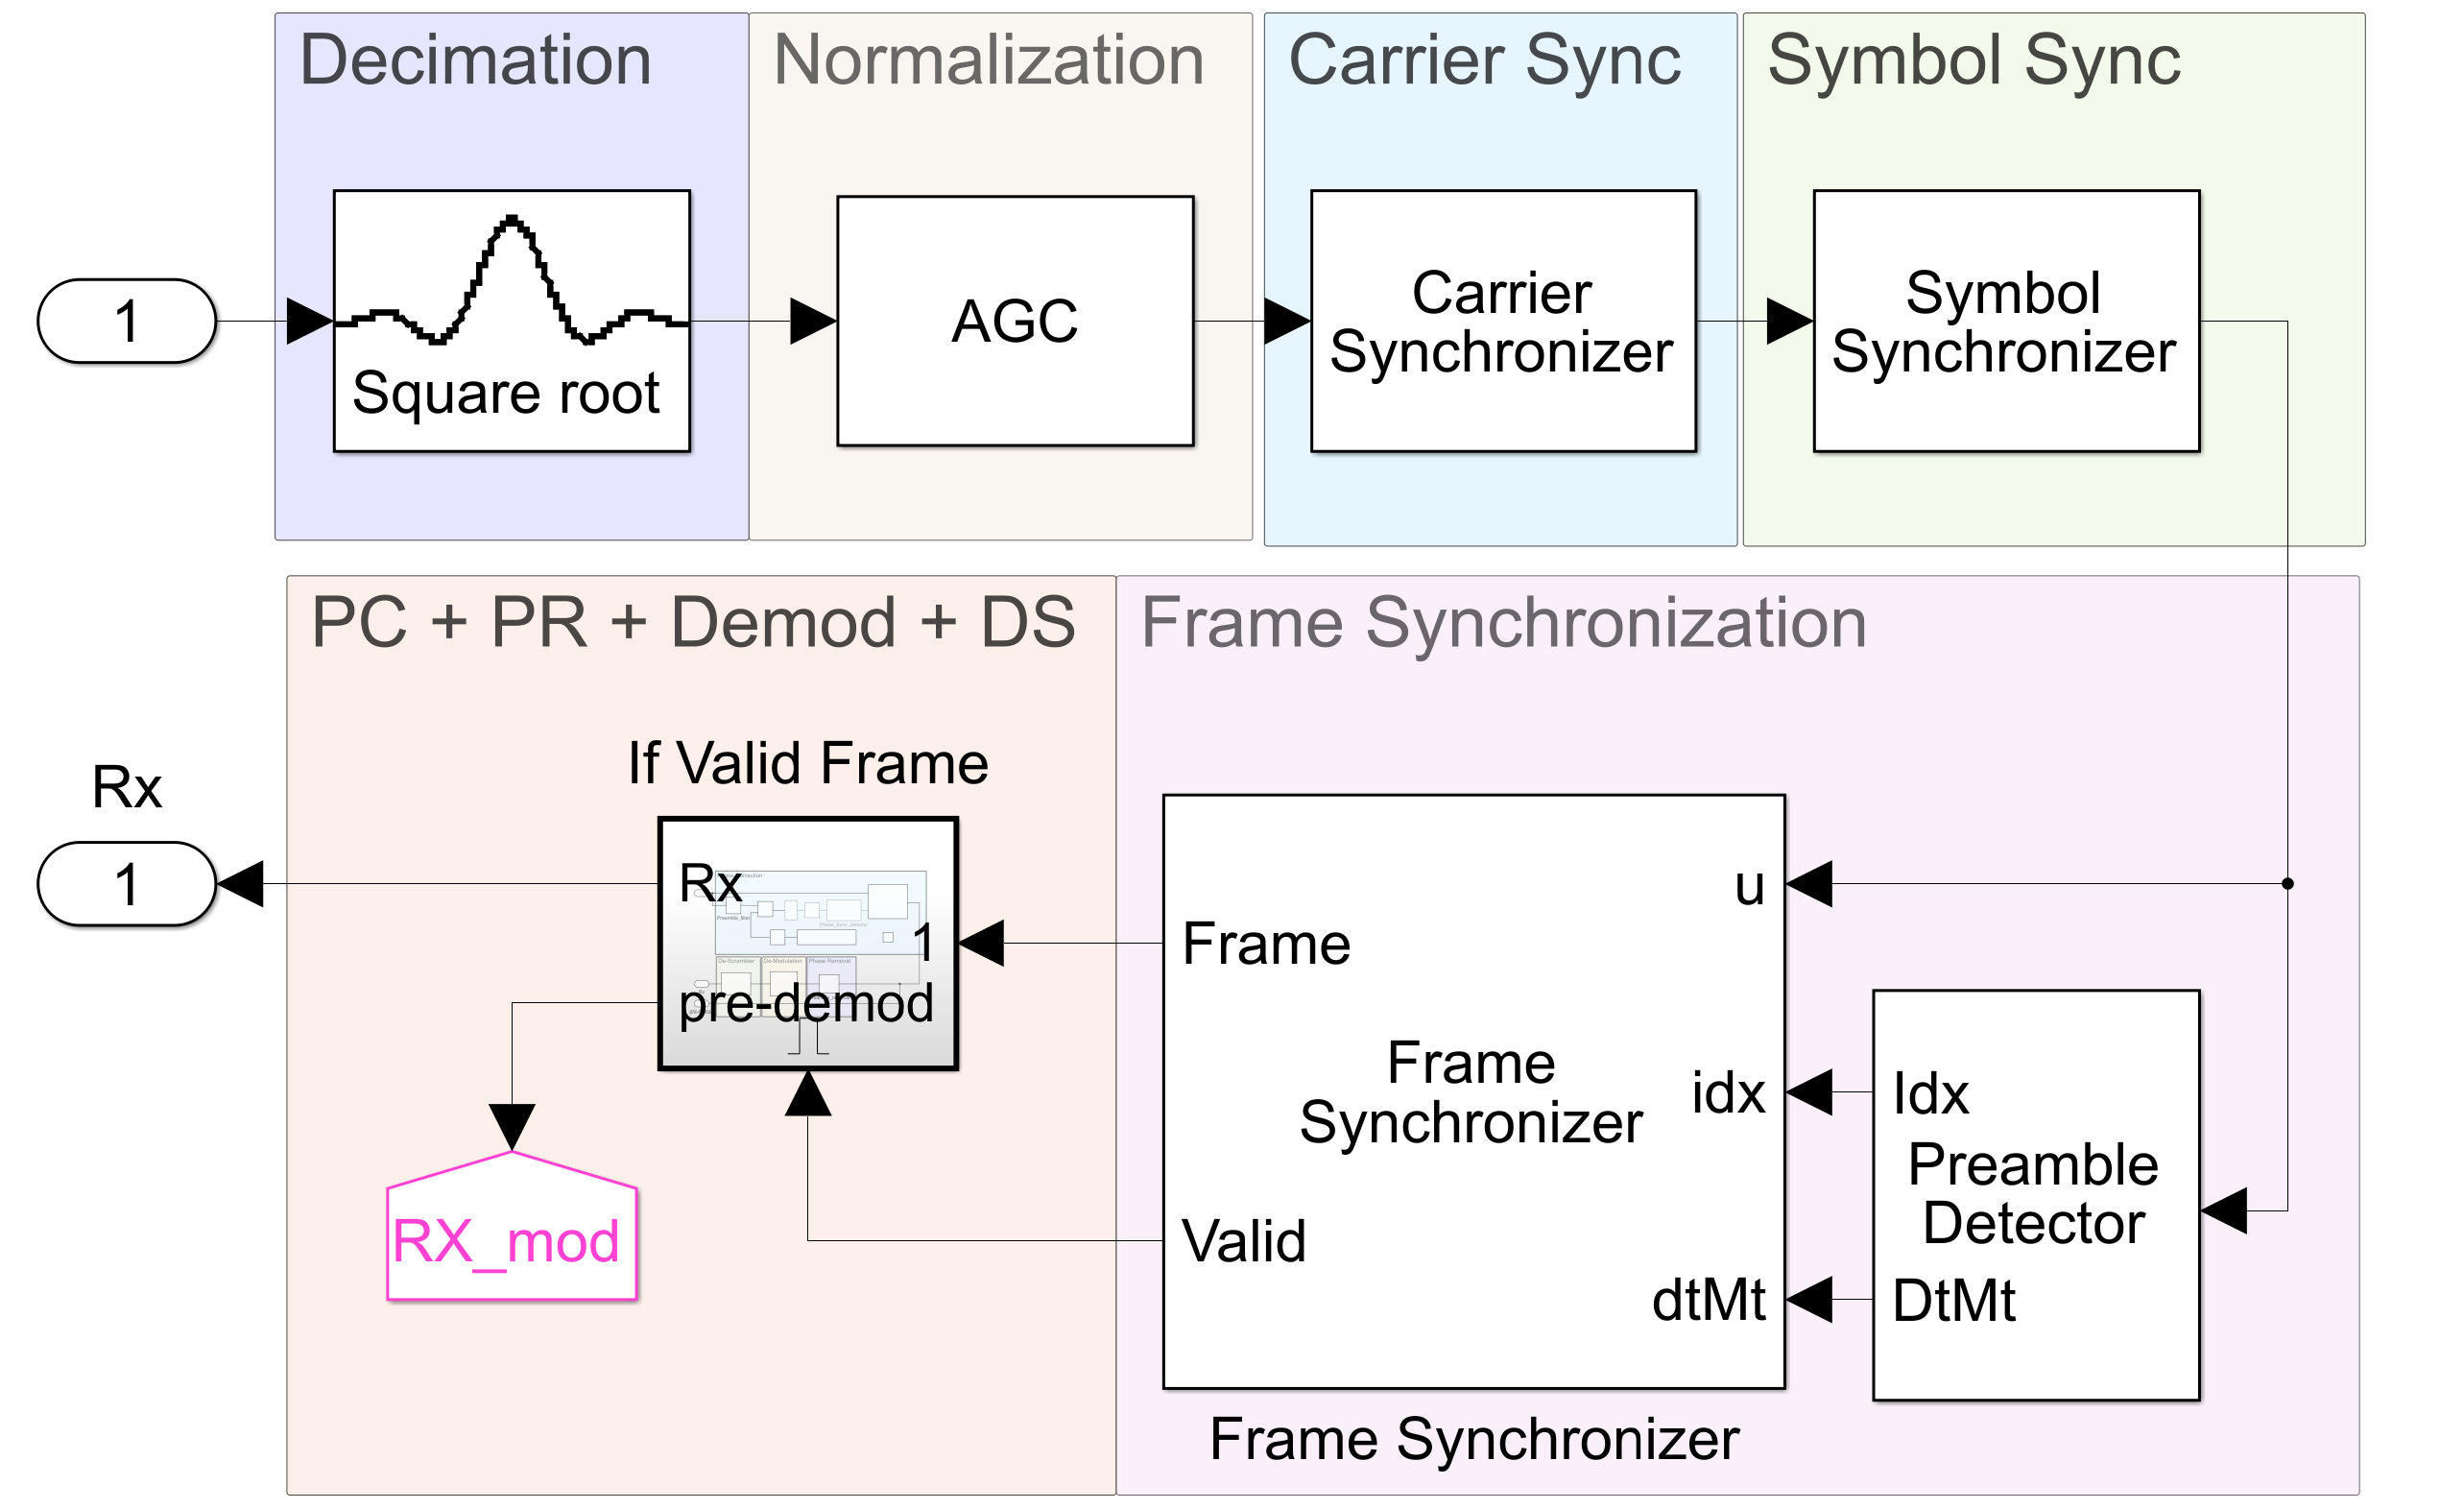
\includegraphics[width = 0.8\textwidth]{Figures/SL_receiver.png}
    \caption[Simulink subsystem for the Receiver.]{Simulink subsystem for the Receiver, part of the model in figure \ref{fig:sim}.}
    \label{fig:sl:receiver}
\end{figure}

\begin{figure}[!]
    \centering
    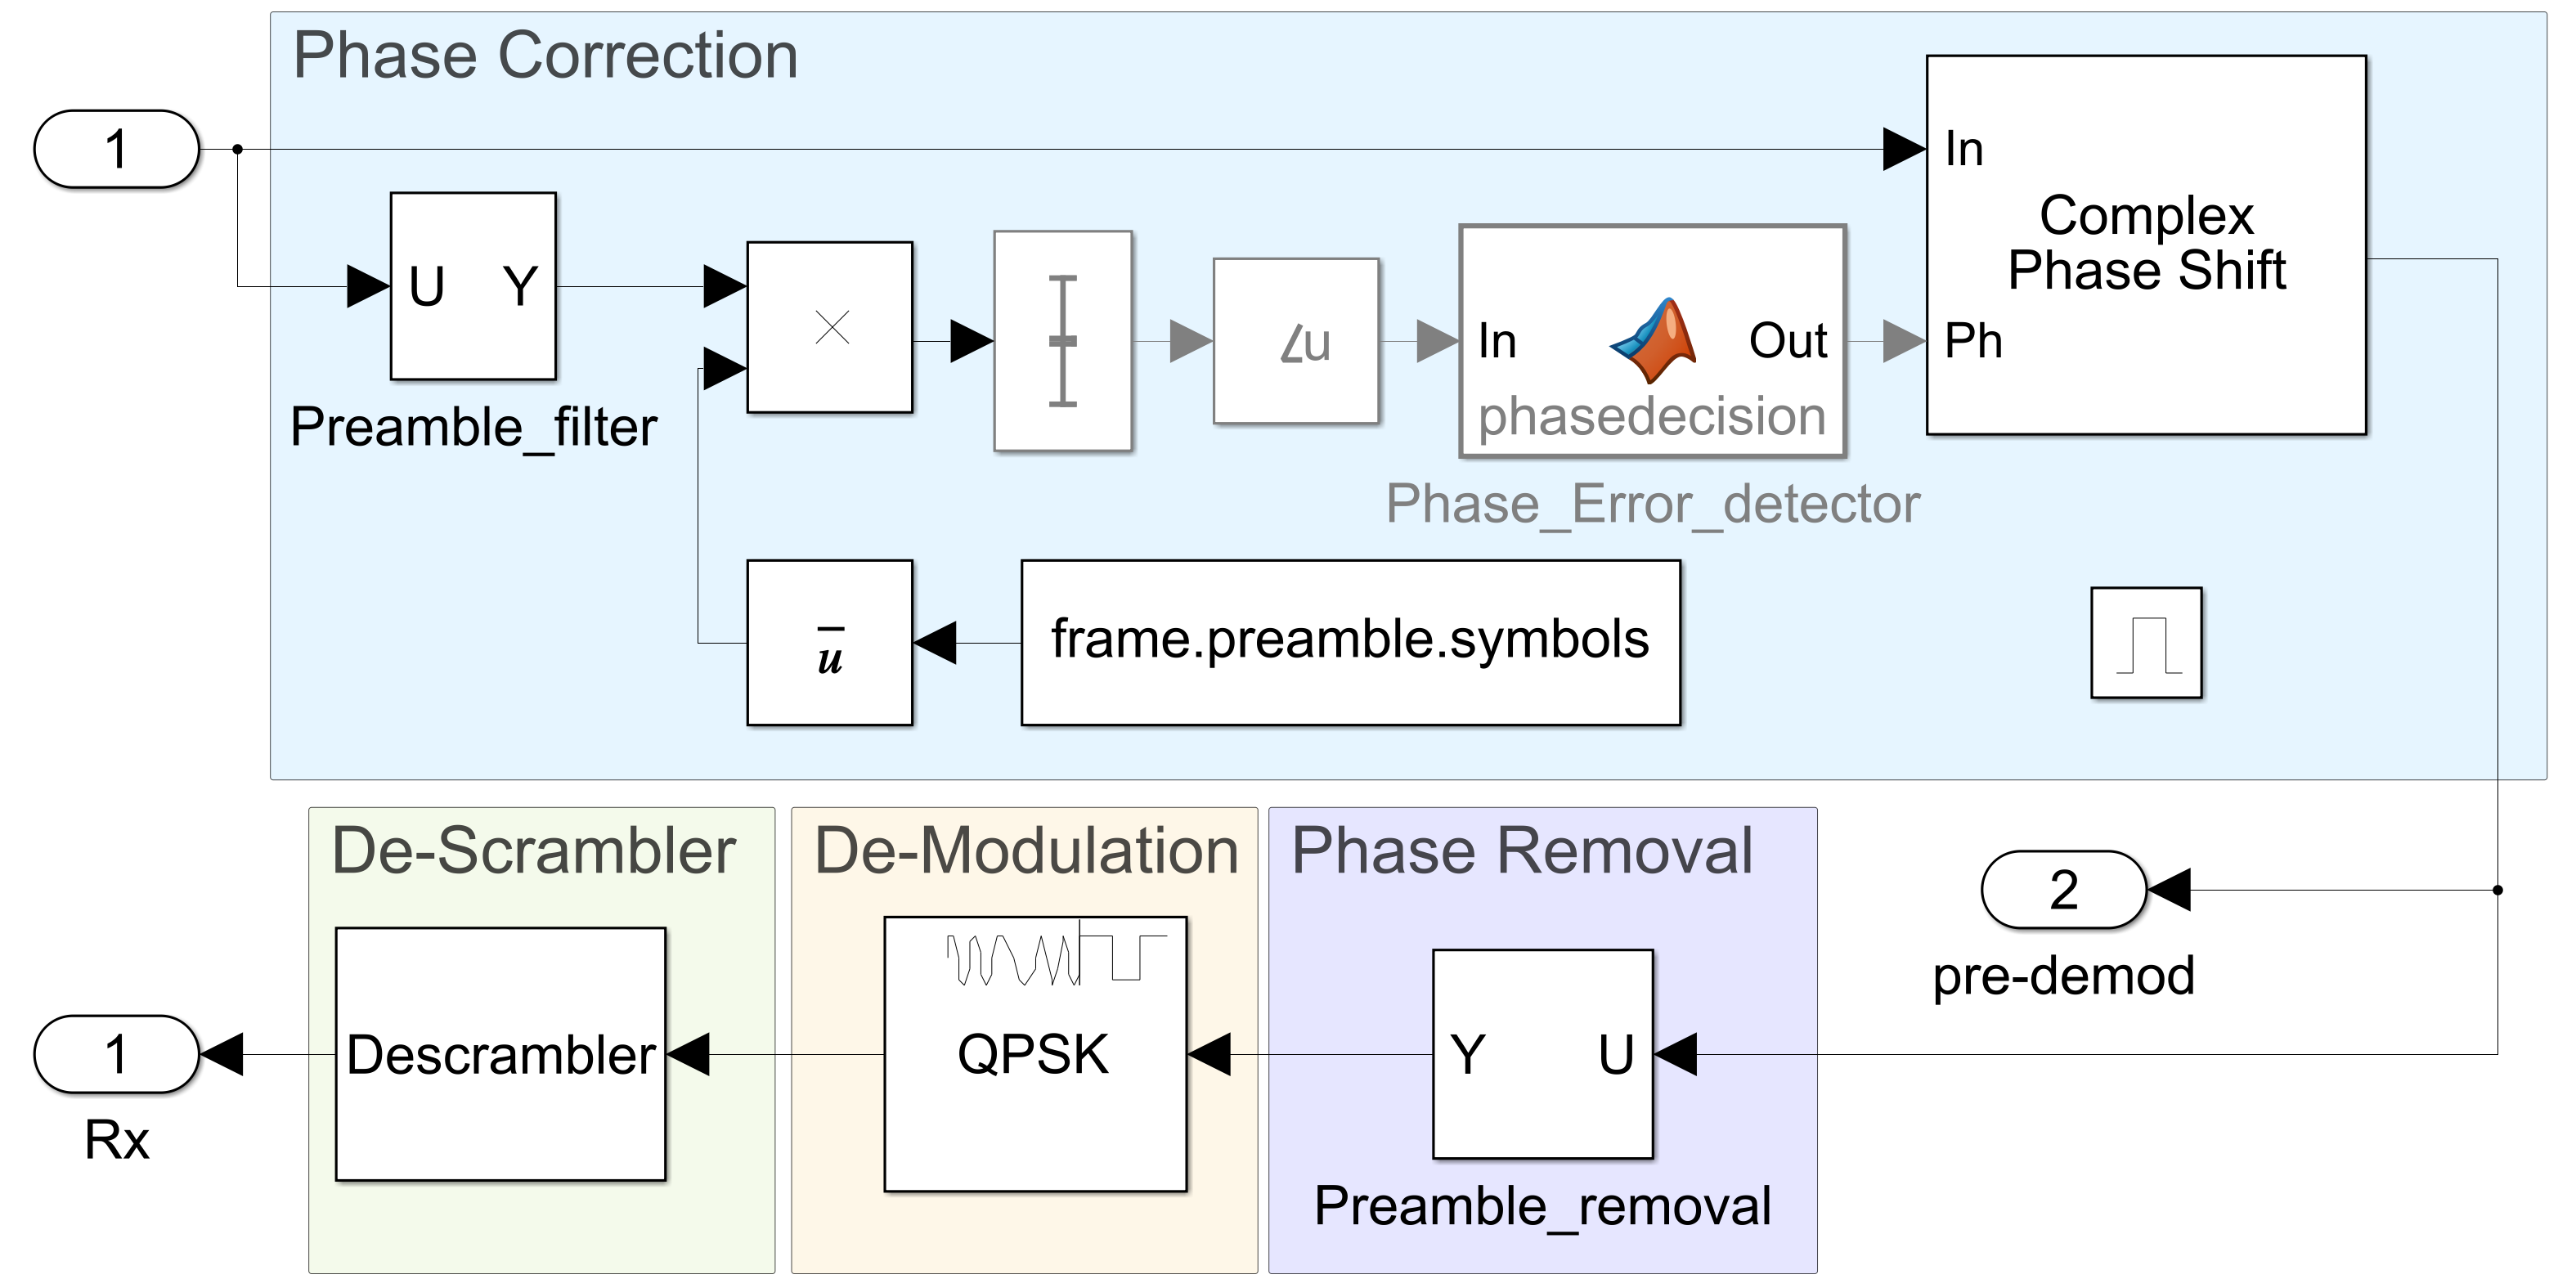
\includegraphics[width = 0.9\textwidth]{Figures/SL_if_valid.png}
    \caption[Simulink subsystem for the valid frame.]{If-valid-Frame Simulink subsystem shown in figure \ref{fig:sl:receiver}.}
    \label{fig:sl:receiver:if_valid}
\end{figure}

\newpage
\subsection{Wireless Channel} \label{met:sim:chan}
An important part of every communications system simulation is the channel model. As this simulation model intends to prove the efficiency of the beamforming algorithm, it only includes Additive White Gaussian Noise (AWGN) components. Some experiments in later sections may include the Simulink subsystem in figure \ref{fig:sl:channel} and other impairments.

The channel subsystem also features the antenna array emulators for the UE and BS, as they affect the signal in different ways. The TX antenna array receives the signal coming from the TX beamformer, which is a [$N_{s/s} \times M$] matrix. This array modifies the signal's gain depending on the actual location of the UE and the beamformer's steering angle; when the TX steering angle roughly matches the UE's angle, the signal will be amplified; otherwise, it will be attenuated.

The RX antenna arrays split the incoming signal into $M$ different signals, one for each antenna element. The AWGN impairment must be added to the split signal, for them to have different added noise signals. The different noise in each element impacts the DOA estimation. The RX antenna array also receives the actual DOA relative to the source device, which will attenuate or amplify the signal depending on the UE's location and the beamformer's steering angle. The receiver antenna array emulator also adds the corresponding phase-shift to the signal sensed by each antenna element according to the beamforming equations in section \ref{back:bf:theoretical}.

\begin{figure}[h]
    \centering
    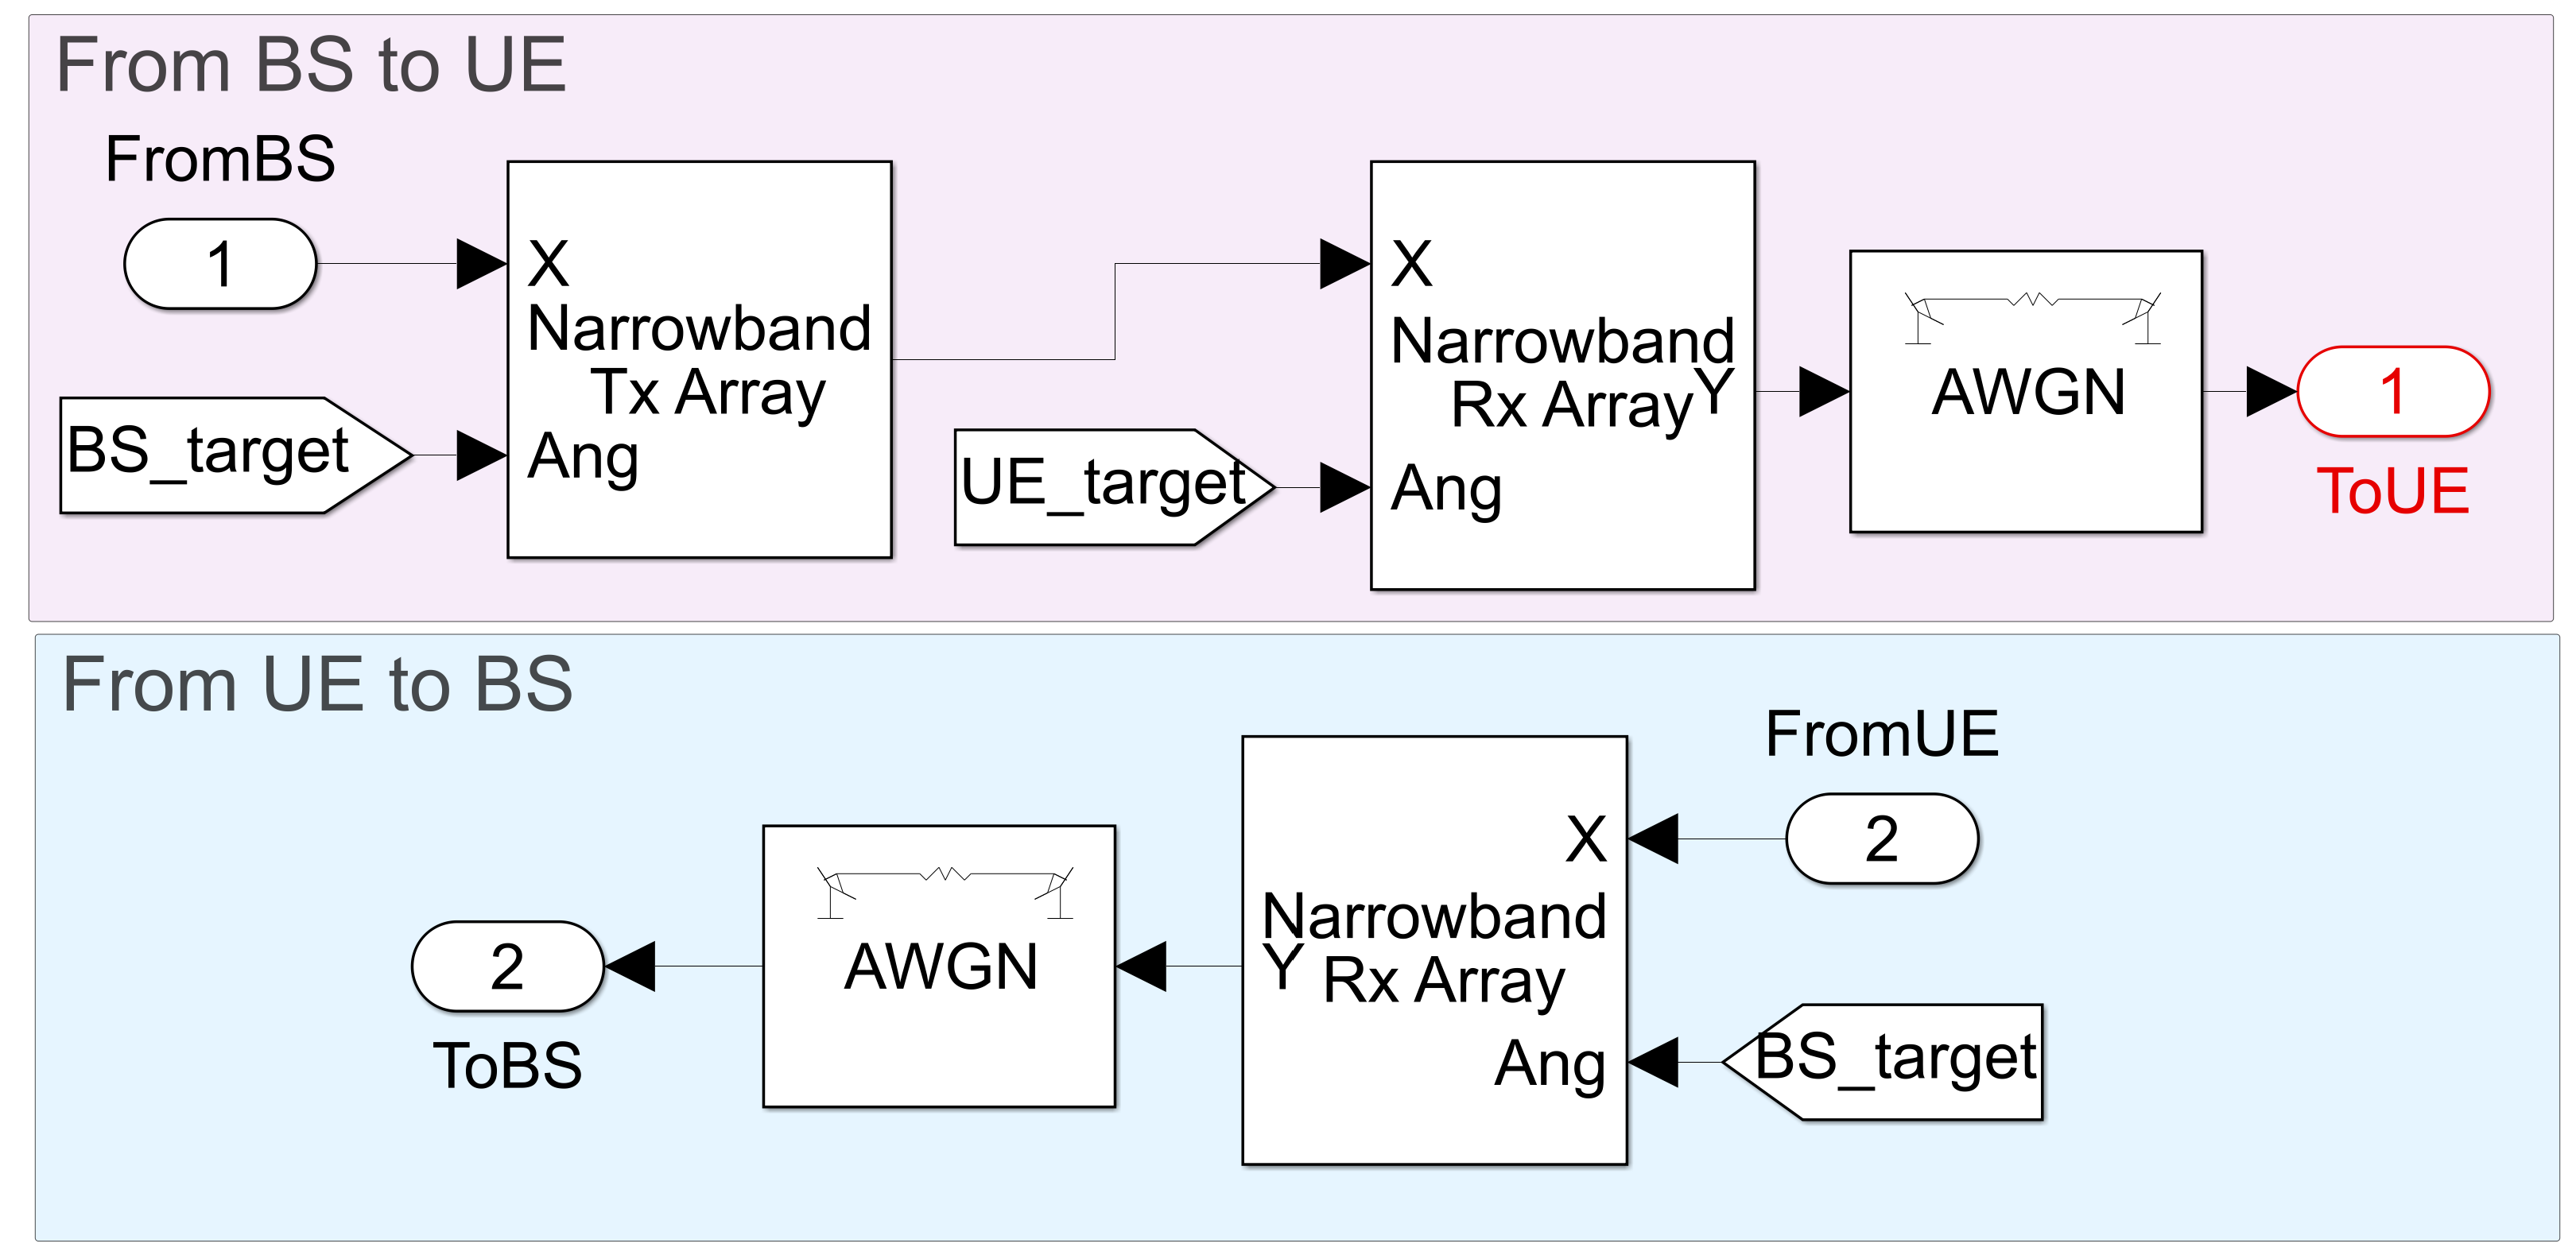
\includegraphics[width = 0.8\textwidth]{Figures/SL_channel.png}
    \caption[Simulink subsystem representing the wireless channel.]{Simulink subsystem representing the wireless channel, part of the model in figure \ref{fig:sim}.}
    \label{fig:sl:channel}
\end{figure}

\newpage
\subsection{Beamformers and Direction of Arrival Estimation} \label{met:sim:bf}
This section describes the design and functionality of the antenna array algorithms as all three of them (two in the BS and one in the UE) perform different tasks. As stated in section \ref{met:problem}, the objective is for the BS to track the UE's movement in order for it to steer its TX beam towards the UE and guarantee a stable link. This task is done by the BS estimating the DOA using the UE's Tx signal and then feeding that signal to the TX beamforming algorithm. Also, the UE supports RX beamforming and is expected to estimate DOA from the BS's TX signal and steer its RX beam towards the BS.

The steering vector of both beamformers is left as an input to make the blocks generic and suitable for other uses as non-adaptive beamforming.

\subsubsection{Receiving Beamformer at the User Equipment} \label{met:sim:bf:rx}
The beamformer at the UE shown in figure \ref{fig:sl:rx_bf} uses the matrix form of equation \ref{eq:combiner_time1} now presented as equation \ref{eq:combiner_time3}, as it only needs an [$N_{s/s} \times M$] matrix representing the signal coming from each element of the antenna array (Obtained from the channel subsystem in section \ref{met:sim:chan}) and [$M \times 1$] vector representing $w_m$. This equation results in a [$N_{s/s} \times 1$] vector representing the beamformed signal.

\begin{equation}
    \textbf{y}(n) = \textbf{x}(n) \textbf{w}^*
    \label{eq:combiner_time3}
\end{equation}

Simulink provides a Phase-Shift beamformer that works for RX beamformers. This block receives the $\textbf{x}(n)$ matrix and a vector containing the DOA and elevation angles; the elevation is assumed to be zero, as stated in section \ref{met:intro}. The beamformer block is used to output the steering weight vector, but only the exponential part of the complex number as in equation \ref{eq:wn}. The block is used this way to enhance its flexibility, as its weights can be combined with a custom $A_m$ vector. As the simulated antenna array obeys equation \ref{eq:distancing}, side lobes are not expected, so the magnitude of the complex vector $\textbf{w}$ is defined as an M-element unitary vector. This system is shown in figure \ref{fig:sl:rx_bf}.

\subsubsection{Transmitting Beamformer at the Base Station} \label{met:sim:bf:tx}
This beamformer in figure \ref{fig:sl:tx_bf}is very similar to the RX beamformer, the input and output signal dimensions are inverted, as this algorithm expects a [$N_{s/s} \times 1$] matrix as input and delivers a [$N_{s/s} \times M$] matrix. The input vector is the signal coming from the Modulator block, and the output matrix columns are the signal to be fed to each antenna element in the array. 

Again, the beamformer block is used to generate the steering vector and recreate the beamforming equations manually. This block requires a [$N_{s/s} \times  M$] matrix only to output the corresponding weights, which is generated by multiplying the input [$N_{s/s} \times 1$] vector times a M-element row vector. The expected behaviour of this subsystem is to receive an estimated DOA from the local RX beamformer that matches the real DOD for the signal being transmitted from the BS is sent towards the UE. This subsystem is shown in figure \ref{fig:sl:tx_bf}. The resulting equation is given by equation \ref{eq:precoder_time} where $\cdot^H$ represents the Hermitian operator.

\begin{equation}
    \textbf{y}(n) = \textbf{x}(n) \textbf{w}^H
    \label{eq:precoder_time}
\end{equation}

\subsubsection{Direction of Arrival Estimation}
The estimated DOA is obtained using the RX antenna array and is used in both the BS and UE. Particularly, the RX antenna array at the BS is used exclusively to estimate the position of the UE. The Simulink subsystem for the DOA estimation is shown in figure \ref{fig:sl:doa}, and is identical for both BS and UE.

The DOA estimator is based on the MUSIC algorithm as this one is more accurate and has a higher resolution than the ESPRIT algorithm \cite{Oumar2012}. This subsystem requires the ULA's parameters to estimate the MUSIC spectrum properly. As stated before, the peaks of the MUSIC spectrum are considered as the DOA. This system is shown in figure \ref{fig:sl:doa}. The output of this block may be used as the steering angle for both beamformers.

\begin{figure}[h]
    \centering
    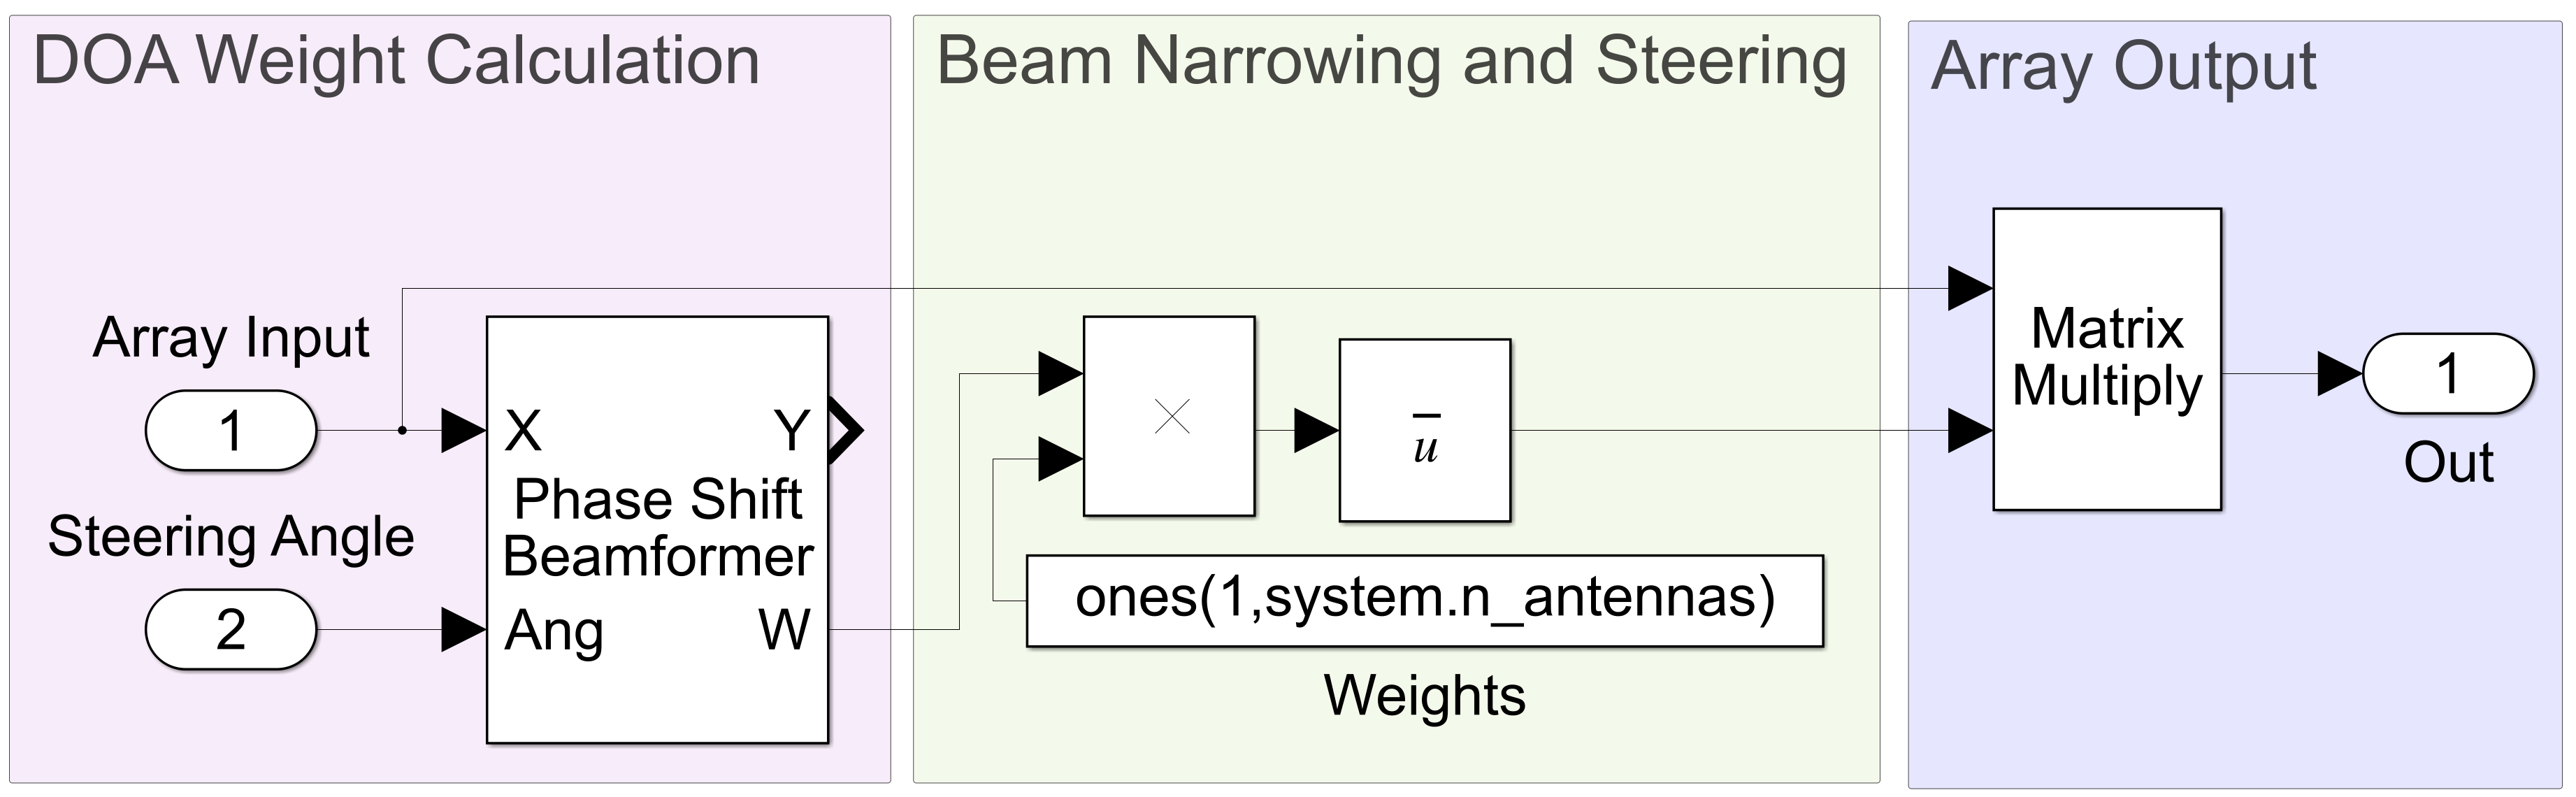
\includegraphics[width = 0.8\textwidth]{Figures/SL_RX_BF.png}
    \caption[Simulink subsystem for the RX beamformer at the UE.]
    {Simulink subsystem for the RX beamformer at the UE, part of the model in \ref{fig:sim}.}
    \label{fig:sl:rx_bf}
\end{figure}

\begin{figure}[h]
    \centering
    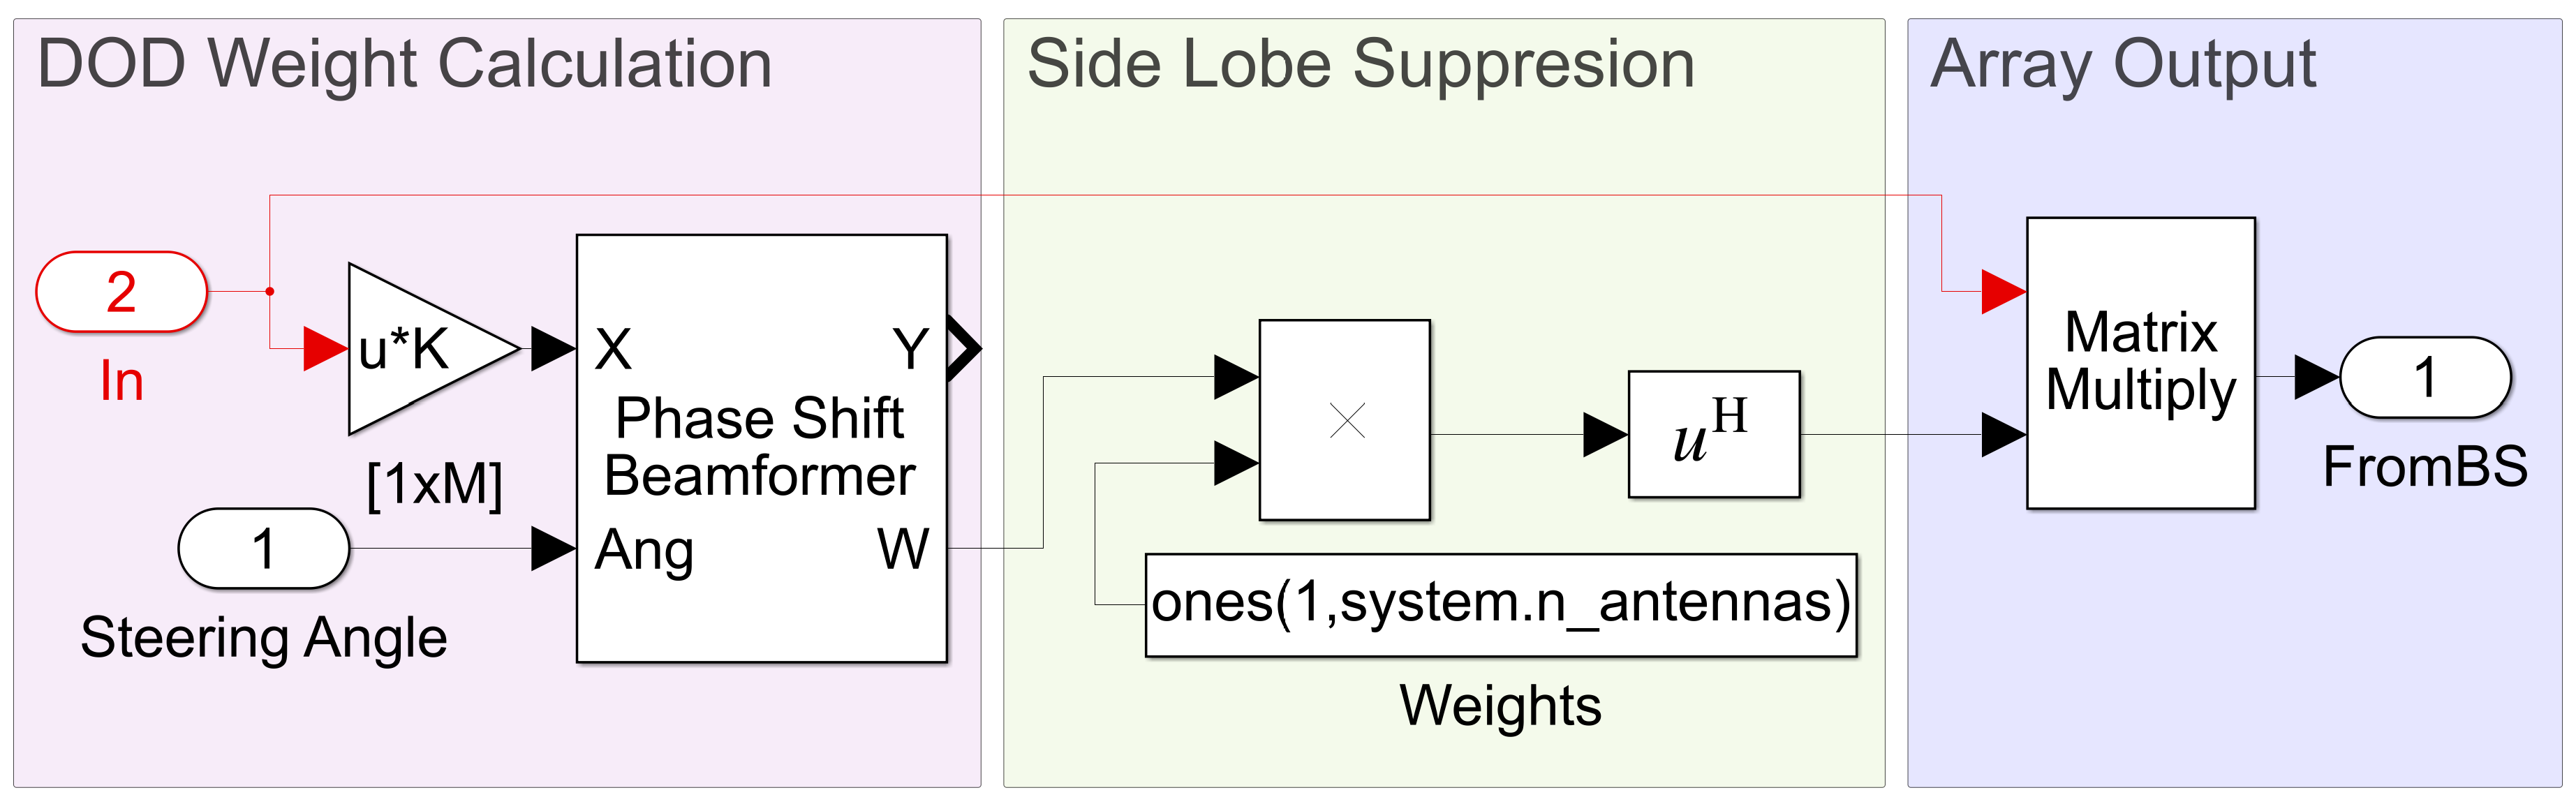
\includegraphics[width = 0.8\textwidth]{Figures/SL_TX_BF.png}
    \caption[Simulink subsystem for the TX beamformer at the BS.]
    {Simulink subsystem for the TX beamformer at the BS, part of the model in figure \ref{fig:sim}.}
    \label{fig:sl:tx_bf}
\end{figure}

\begin{figure}[!h]
    \centering
    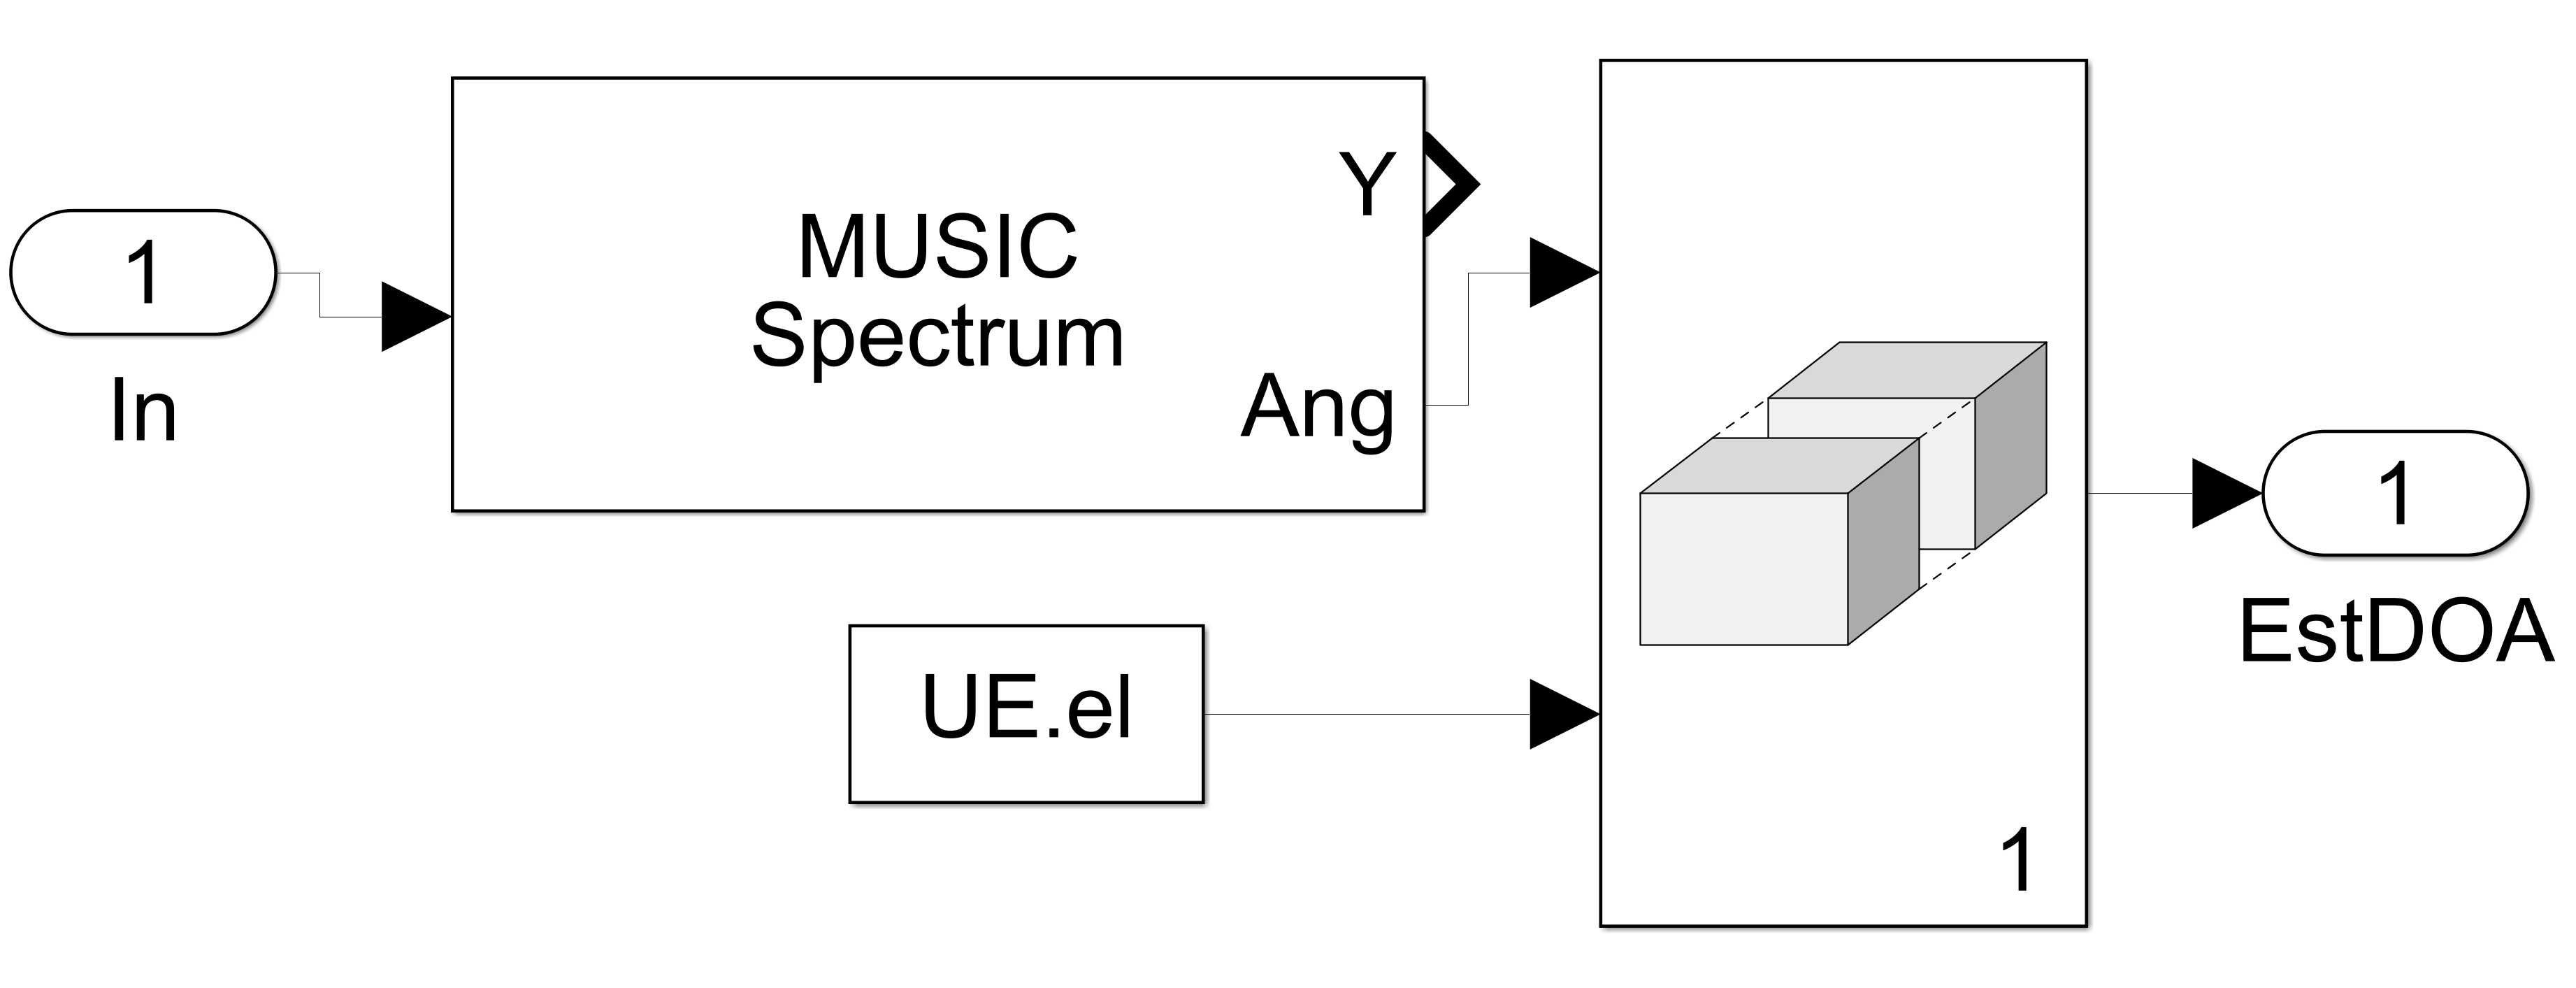
\includegraphics[width = 0.5\textwidth]{Figures/SL_doa.png}
    \caption[Simulink subsystem for the DOA estimation.]{Simulink subsystem for the DOA estimation, part of the model in figure \ref{fig:sim}.}
    \label{fig:sl:doa}
\end{figure}

\newpage
\section{SDR Selection} \label{met:sdr}
\subsection{Introduction} \label{met:sdr:intro}
This section describes the requirements of the beamforming algorithm for it to be executed in a SDR and the characteristics and features of the selected unit. The filtering and analysis of each unit was done based in the content from sections \ref{back:bf:theoretical}, \ref{back:sdr:avail} and \ref{back:bf_sdr}. The best SDR candidates are listed in table \ref{tb:SDRcomp}.

\subsection{Requirements} \label{met:sdr:req}
As stated in section \ref{back:sdr:avail}, many SDR units are varying in cost and performance. Some of the presented options are low-cost and intended to be used for learning or just as a cost-effective alternative to higher-end products as the Ettus Research devices. 

\subsubsection{MIMO} \label{met:sdr:req:mimo}
Beamforming is a spatial diversity technique, meaning that the most obvious requirement for the SDR to have is MIMO capabilities (More than one antenna at the transmitter or receiver end). This requirement is the most important, as the beamforming equations require many coherent signal sources.

SDRs such as the Ettus B210, LimeSDR and BladeRF would be obvious choices considering the previous constraint; as all of these support 2x2 MIMO or even 4x4 as is the case of the PCI version of the LimeSDR. However, hardware modifications and can be done to the HackRF \cite{Edgcombe2019MultipleSynchronization}, RTL-SDR \cite{Laakso2018Phase-coherentBeamforming, Myrick2018DistributedRadios, Othernet2019KerberosSDR} and PlutoSDR \cite{CoherentReceiver2020CoherentSDR} to support coherent streams. These modifications vary in difficulty and resulting performance and may not be suitable to modify a device only to serve this purpose permanently.

\subsubsection{Transfer Speed} \label{met:sdr:req:ts}
As stated in section \ref{back:bf_sdr:int}, spatial diversity applications require high-speed data transfers to guarantee a deterministic performance. Many parts of the end-to-end simulation, especially the receiver, would be broken if the SDR's RX buffer overflows. A reliable data transfer is expected from the SDR even using its MIMO scheme; this requires a reliable communication protocol such as USB3.0, PCI and Ethernet.

Again, the mid-high tier SDRs satisfy this requirement, as the Ettus B210, LimeSDR and BladeRF all support USB3.0.

\subsubsection{Software Support} \label{met:sdr:req:soft}
This requirement is essential if the development cycle is based on MBD or HIL. The community maintains many of these SDRs, so their software support is not official and is not expected to work flawlessly or to exploit all the capabilities of the device. This requirement is satisfied by the most available and the units backed by companies such as the Ettus B210, RTL-SDR, PlutoSDR and BladeRF.

\subsection{Selected Hardware} \label{met:sdr:sel}
Only two of the listed SDRs satisfied all three requirements: The Ettus Research's B210 and Nuand's BladeRF 2.0 A4. The latter SDR is the one selected as the B210 is considered a baseline to what low-cost SDR unis should offer.

The BladeRF is a mid-tier SDR containing an Altera Cyclone IV FPGA, an Analog Devices' AD9361 RF transceiver (as the one shown in figure \ref{fig:ad9361}) and a Cypress FX3 USB3.0 SuperSpeed controller; as shown in figure \ref{fig:bladerf}. It supports 2x2 MIMO and also can be linked to another BladeRF, maintaining pseudo-coherence to achieve 4x4 MIMO. Finally, it has support for C/C++, Python, GNU-Radio and MATLAB/Simulink (1x1 SISO). 

The simulation scenarios in chapter \ref{test} consider this SDR's characteristics and features in the equations in section \ref{met:sim}, these are shown in table \ref{tab:bladerf}.

\begin{figure}
    \centering
    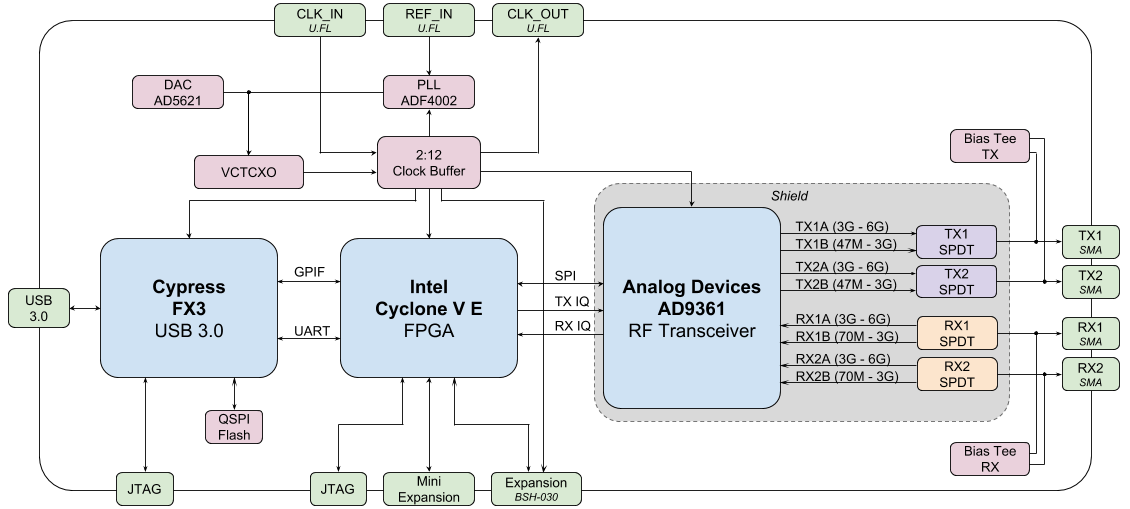
\includegraphics[width = \textwidth]{Figures/bladerf_bd.png}
    \caption{BladeRF 2.0 A4 block diagram. \cite{Nuand2018BladeRFMicro}}
    \label{fig:bladerf}
\end{figure}



\begin{table}
    \centering
    \begin{tabular}{c|c|c|c}
        Parameter & Minimum & Nominal & Maximum \\ \hline
        MIMO ($M$) & - & 2 & - \\ 
        Sampling Rate ($f_{bb}$) & 521 kSPS & - & 61.44 MSPS \\ 
         TX RF Tuning Frequency ($f_c$) & 70 MHz & - & 6 GHz \\ 
         RX RF Tuning Frequency ($f_c$) & 47 MHz & - & 6 GHz \\ 
         TX Power & - & - & 8 dBm \\
    \end{tabular}
    \caption{BladeRF's RF specifications. \cite{Nuand2018BladeRFMicro}}
    \label{tab:bladerf}
\end{table}

\newpage
\section{Hardware Interface for MATLAB/Simulink} \label{met:int}
The BladeRF supports MATLAB and Simulink bindings of the C/C++, allowing using the SDR within these software packages. As the first tests using the SDR, a communication system based on the Modulator and Receiver block was developed. By using the previous blocks with the Simulink system-object provided by Nuand, it was certain that these SDR blocks do not support 2x2 MIMO, which was a requirement for the following tests. The problem that this section tackle is the development of a MIMO interface for the BladeRF so that it can be used in the demonstration model. 

The resulting MATLAB and Simulink scripts are based on the provided source code and the documentation for the C/C++ library. Although this script is built based on what is provided, the community interested in the BladeRF would greatly benefit from this effort.

\subsection{libbladeRF} \label{met:int:lib}
Nuand's libbladeRF is the official interface library for the BladeRF in C/C++. Their Doxygen site \cite{Nuand2019LibbladeRF2.2.1} describes the use of each module of the API, including some examples of 1x1 setup and boilerplate code. The template code describes a setup sequence to follow and how to use the synchronous interface for transmitting and receiving signals; this sequence is described in the flowchart in figure \ref{fig:flowchart}.

\begin{figure}[h]
    \centering
    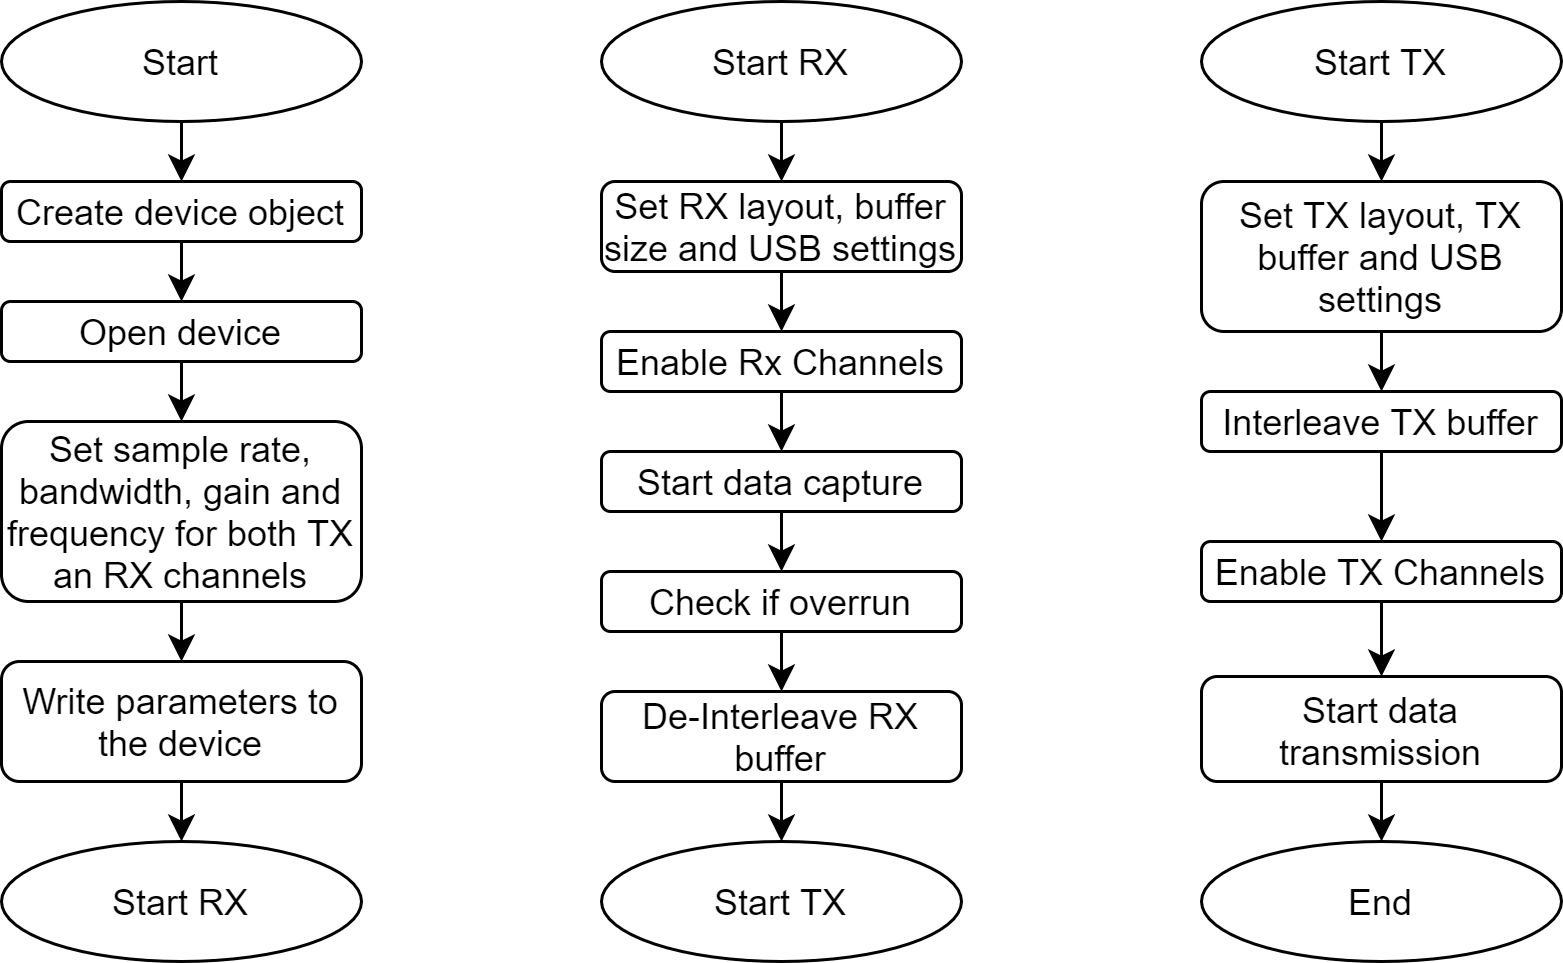
\includegraphics[width = 0.7\textwidth]{Figures/bladerf_flowchart.png}
    \caption{Device setup and utilisation. \cite{Nuand2019LibbladeRF2.2.1}}
    \label{fig:flowchart}
\end{figure}

\subsubsection{Initial Configuration} \label{met:int:lib:init}
The first step of the template is to create a device object using the \verb|bladerf_devinfo| and \verb|bladerf| structures and the \verb|bladerf_init_devinfo| function. Then, the sample rate, bandwidth, gain and tuning frequency are written to each channel using the \verb|bladerf| structure; this process must be repeated for every intended channel, being four times for 2x2 MIMO. After this step, the individual RX and TX front-ends can be configured and used. \cite{Nuand2019LibbladeRF2.2.1}

\subsubsection{Front-End Configuration and Data handling} \label{met:int:lib:rx}
The next step is to configure both TX and RX channels by using the \verb|bladerf_sync_config| function and the device structure. The required parameters for this functions are the layout, the USB transfer parameters and the sample format; the first is a macro definition which defines the layout the front-end will have (Using RX0, RX1 or both; same logic with TX) and the second are four parameters that describe the USB transfer buffer size, number of buffers and timeout. Lastly, the format parameter denotes the use of metadata for synchronous transfers. After configuring the RX front-end, the user must enable the channels configured in the last step of section \ref{met:int:lib:init} using the \verb|bladerf_enable_module|. 

The receiving process is triggered using the \verb|bladerf_sync_rx|, which fills the RX buffer with the received samples. The number of received samples parameter in the previous function is the total number of samples received for all the channels, and the RX buffer must be twice the size to hold the samples if both channels are used. The received samples are given in the Signed-Complex 16-bit Q11 (SC16Q11) format and must be de-interleaved as described in section \ref{met:int:lib:sc16q11} before processing them. The overrun flag may be set if the size of the received data does not equal the expected size. \cite{Nuand2019LibbladeRF2.2.1}

The transmission is done similar to the reception, and the TX buffer must be interleaved to match the SC16Q11 format and then transmitted using the \verb|blade_sync_tx| function.

\subsubsection{Signed-Complex 16-bit Q11 Format} \label{met:int:lib:sc16q11}
This format is widely used in industrial instrumentation and is a standard way to organise data from several ADCs or going so several DACs. BladeRF's libbladeRF handles all the data going through the ADCs and DACs using this format, meaning that the user must make sure that the TX buffer is interleaved before calling \verb|bladerf_sync_tx| and de-interleave the received samples after calling \verb|bladerf_sync_rx|.

The SC16Q11 format uses 16-bit signed integers to represent the I and Q components of the samples and packs both numbers into a single 32-bit integer. This packed sample is little-endian, and the first 16 bits correspond to the I sample and the last 16 bits to the Q sample. The order of samples is also important for the format, as the first 32-bit integer in the buffer represents sample 0 of channel 0, the second integer represents sample 0 of channel 1 and so on. A summary of the SC16Q11 format is given in table \ref{tab:sc16q11}. \cite{Nuand2019LibbladeRF2.2.1}

\begin{table}[h]
    \centering
    \begin{tabular}{c|c|c|c}
        Byte offset & Bit 31 - 16 & Bit 15 - 0 & Description\\ \hline
        0x00 & $Q_0(0)$ & $I_0(0)$ & Ch 0, sample 0 \\
        0x04 & $Q_1(0)$ & $I_1(0)$ & Ch 1, sample 0 \\
        0x08 & $Q_0(1)$ & $I_0(1)$ & Ch 0, sample 1 \\
        0x0C & $Q_1(1)$ & $I_1(1)$ & Ch 1, sample 1 \\
        0x10 & $Q_0(2)$ & $I_0(2)$ & Ch 0, sample 2 \\
        0x14 & $Q_1(2)$ & $I_1(2)$ & Ch 1, sample 2 \\
        ... & ... & ... & ... \\
        $2 (N_{s/s}-1) \times \text{0x04}$ & $Q_0(N_{s/s}-1)$ & $I_0(N_{s/s}-1)$ & Ch 0, sample $N_{s/s}$ \\
        $2 (N_{s/s}-1) \times \text{0x04}+ 1$ & $Q_1(N_{s/s}-1)$ & $I_1(N_{s/s}-1)$ & Ch 1, sample $N_{s/s}$ \\
    \end{tabular}
    \caption[SC16Q11 layout example for 2 channels.]{SC16Q11 layout example for 2 channels. \cite{Nuand2019LibbladeRF2.2.1}}
    \label{tab:sc16q11}
\end{table}

\subsection{MATLAB System Object} \label{met:int:mat}
The MATLAB script provided by Nuand performs a process similar to the one described in the previous section. The main difference is that only a single channel in either the TX or RX front-is active at any time, defying the definition of the MIMO scheme. Since the MATLAB script is a binding script to the libbladeRF API, the same approach described in section \ref{met:int:lib} can be programmed while conserving most of the existing code. The challenge of this step was to read through the existing MATLAB script, find where each section of the algorithm takes place and do the necessary changes.

The changes made to the original version of the scrip were copied into a separate file with a different system object called \verb|bladeRF_MIMO|. This new object performs the initial steps, but for both channels, always. The entire front-ends can be enabled or disabled independently, but if enabled, both channels are active, and all the configuration is applied to both channels; although the gain can be set independently if the onboard AGC is not enabled. The channel layout macro was changed at the front-end configuration to use both channels simultaneously. Also, the interleaving and de-interleaving stages had to be handled manually in MATLAB.

The new script now can receive and output a [$N_{s/s} \times 2$] matrix, where each column is the data being transmitted or received by each channel and the rows represent the sample number.

Simulink requires an additional wrapper object for the object to be compatible with the other blocks, as Simulink often compiles the blocks in the model for them to be executed efficiently, opposed to MATLAB's interpreted execution.

\newpage
\section{Antenna Mounting} \label{met:mount}
Beamforming requires that the antenna elements in the array are placed at a constant distance given by equation \ref{eq:distancing} to avoid spatial aliasing. Placing the antennas at a known distance is also a requirement for the DOA estimation, which requires the array distancing and operative frequency to estimate the DOA properly. These reasons were enough to build a structure that holds the SDR's antennas in place. This structure was designed using Fusion 360 (A CAD/CAM/CAE software) to make the manufacture and reproduction of this work easier.

The CAD model; similar to the mathematical model in the simulation (section \ref{met:sim}) is a parametric model that changes its geometry according to the input parameters. These parameters are the carrier frequency $f_c$ and number of antenna elements $M$. The carrier frequency determines the distance between elements as described in equation \ref{eq:distancing}, as it assumes the placement to be optimal. Other parameters as the mast height and the lip height are considered input parameters.

\begin{equation*}
    d = \frac{\lambda}{2} = \frac{c}{2f_c}
\end{equation*}

The structure has three main components, a circular base, mast and the beam. The base holds the structure and its diameter must maintain the antenna array in place without falling. The mast links the base and the beam; while routing the cables to each antenna element inside of it. The beam holds the antennas using little indentations in the lip above the beam. The antennas are supposed to be placed using zip ties. Most of the dimensions of depend on the $f_c$ and $M$ as shown in figures \ref{fig:tb_cad}.

\begin{table}[h]
    \centering
    \begin{tabular}{c|c|c|c|c}
        Parameter & Formula & $f_c = 890 \text{ MHz}$ & $f_c = 430 \text{ MHz}$ & $f_c = 2.4 \text{ GHz}$, $M = 4$\\ \hline
        Antenna distancing & $d = \lambda/2$ & 168.42 & 348.59 & 62.45\\
        Beam length & $L_{beam} = 1.15 \:d\: (M-1) $ & 197.72 & 409.25 & 73.32\\
        Beam width & $W_{beam} = 0.35 \: (M-1)^{-0.7}$ & 69.20 & 143.23 & 25.66\\
        Mast diameter & $d_{mast} = 0.625 W_{beam}$ & 43.25 & 89.52 & 16.04\\
        Base diameter & $d_{base} = 0.8 L_{beam}$ & 158.18 & 327.40 & 58.69\\
    \end{tabular}
    \caption[Formulas for the parametric design of the antenna holder.]{Formulas used to determine each length in the structure and examples for different frequencies. Units are in millimetres and $M = 2$ unless specified.}
    \label{tab:tb_cad}
\end{table}

\begin{figure}[h]
    \centering
    \begin{subfigure}{0.3\textwidth}
        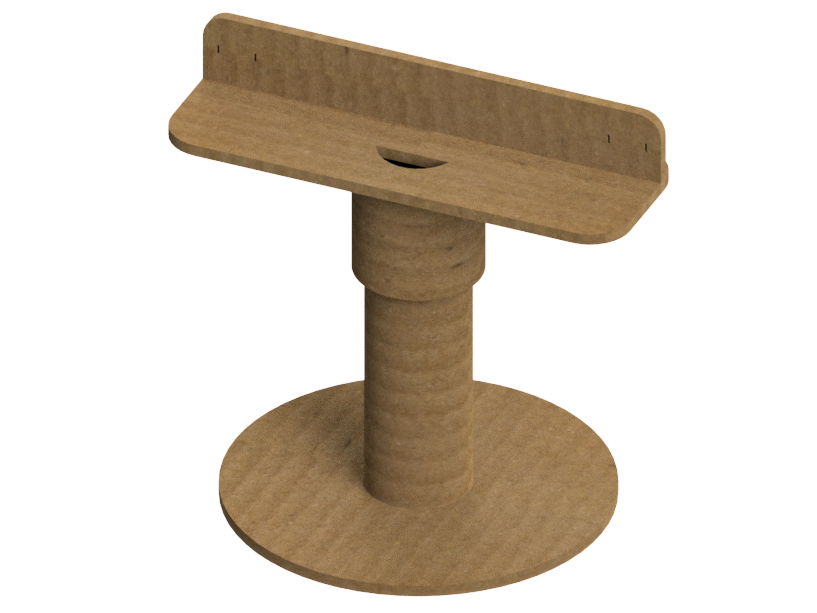
\includegraphics[width = \textwidth]{Figures/tb_cad_890.png}
        \caption{$f_c = 890 \text{ MHz}$, $M = 2$}
    \end{subfigure}
    \begin{subfigure}{0.3\textwidth}
        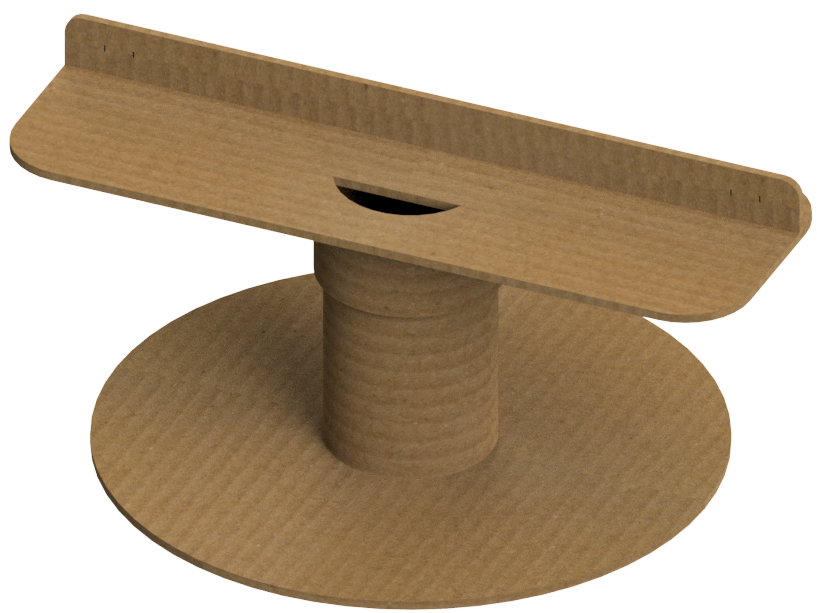
\includegraphics[width = \textwidth]{Figures/tb_cad_430.png}
        \caption{$f_c = 430 \text{ MHz}$, $M = 2$}
    \end{subfigure}
    \begin{subfigure}{0.3\textwidth}
        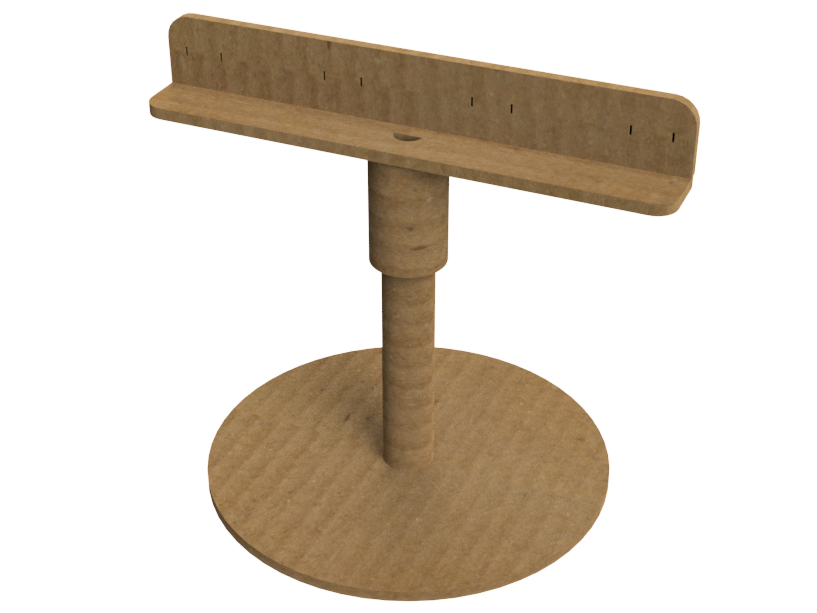
\includegraphics[width = \textwidth]{Figures/tb_cad_2400.png}
        \caption{$f_c = 2.4 \text{ GHz}$, $M = 4$}
    \end{subfigure}
    \caption[Antenna holder example structures.]{Examples of different antenna structures for various carrier frequencies and antenna elements. The mast height remains constant across experiments to appreciate the differences.}
    \label{fig:tb_cad}
\end{figure}

Two structures were manufactured using cardboard boxes, as this material was available at the time. The used parameters were $f_c = 890$ MHZ, $M = 2$, mast height of 150 mm and lip length of 30 mm. The carrier frequency was chosen using an unused section in the UK's ISM band, which results in a relatively small structure.

\begin{figure}[!]
    \centering
    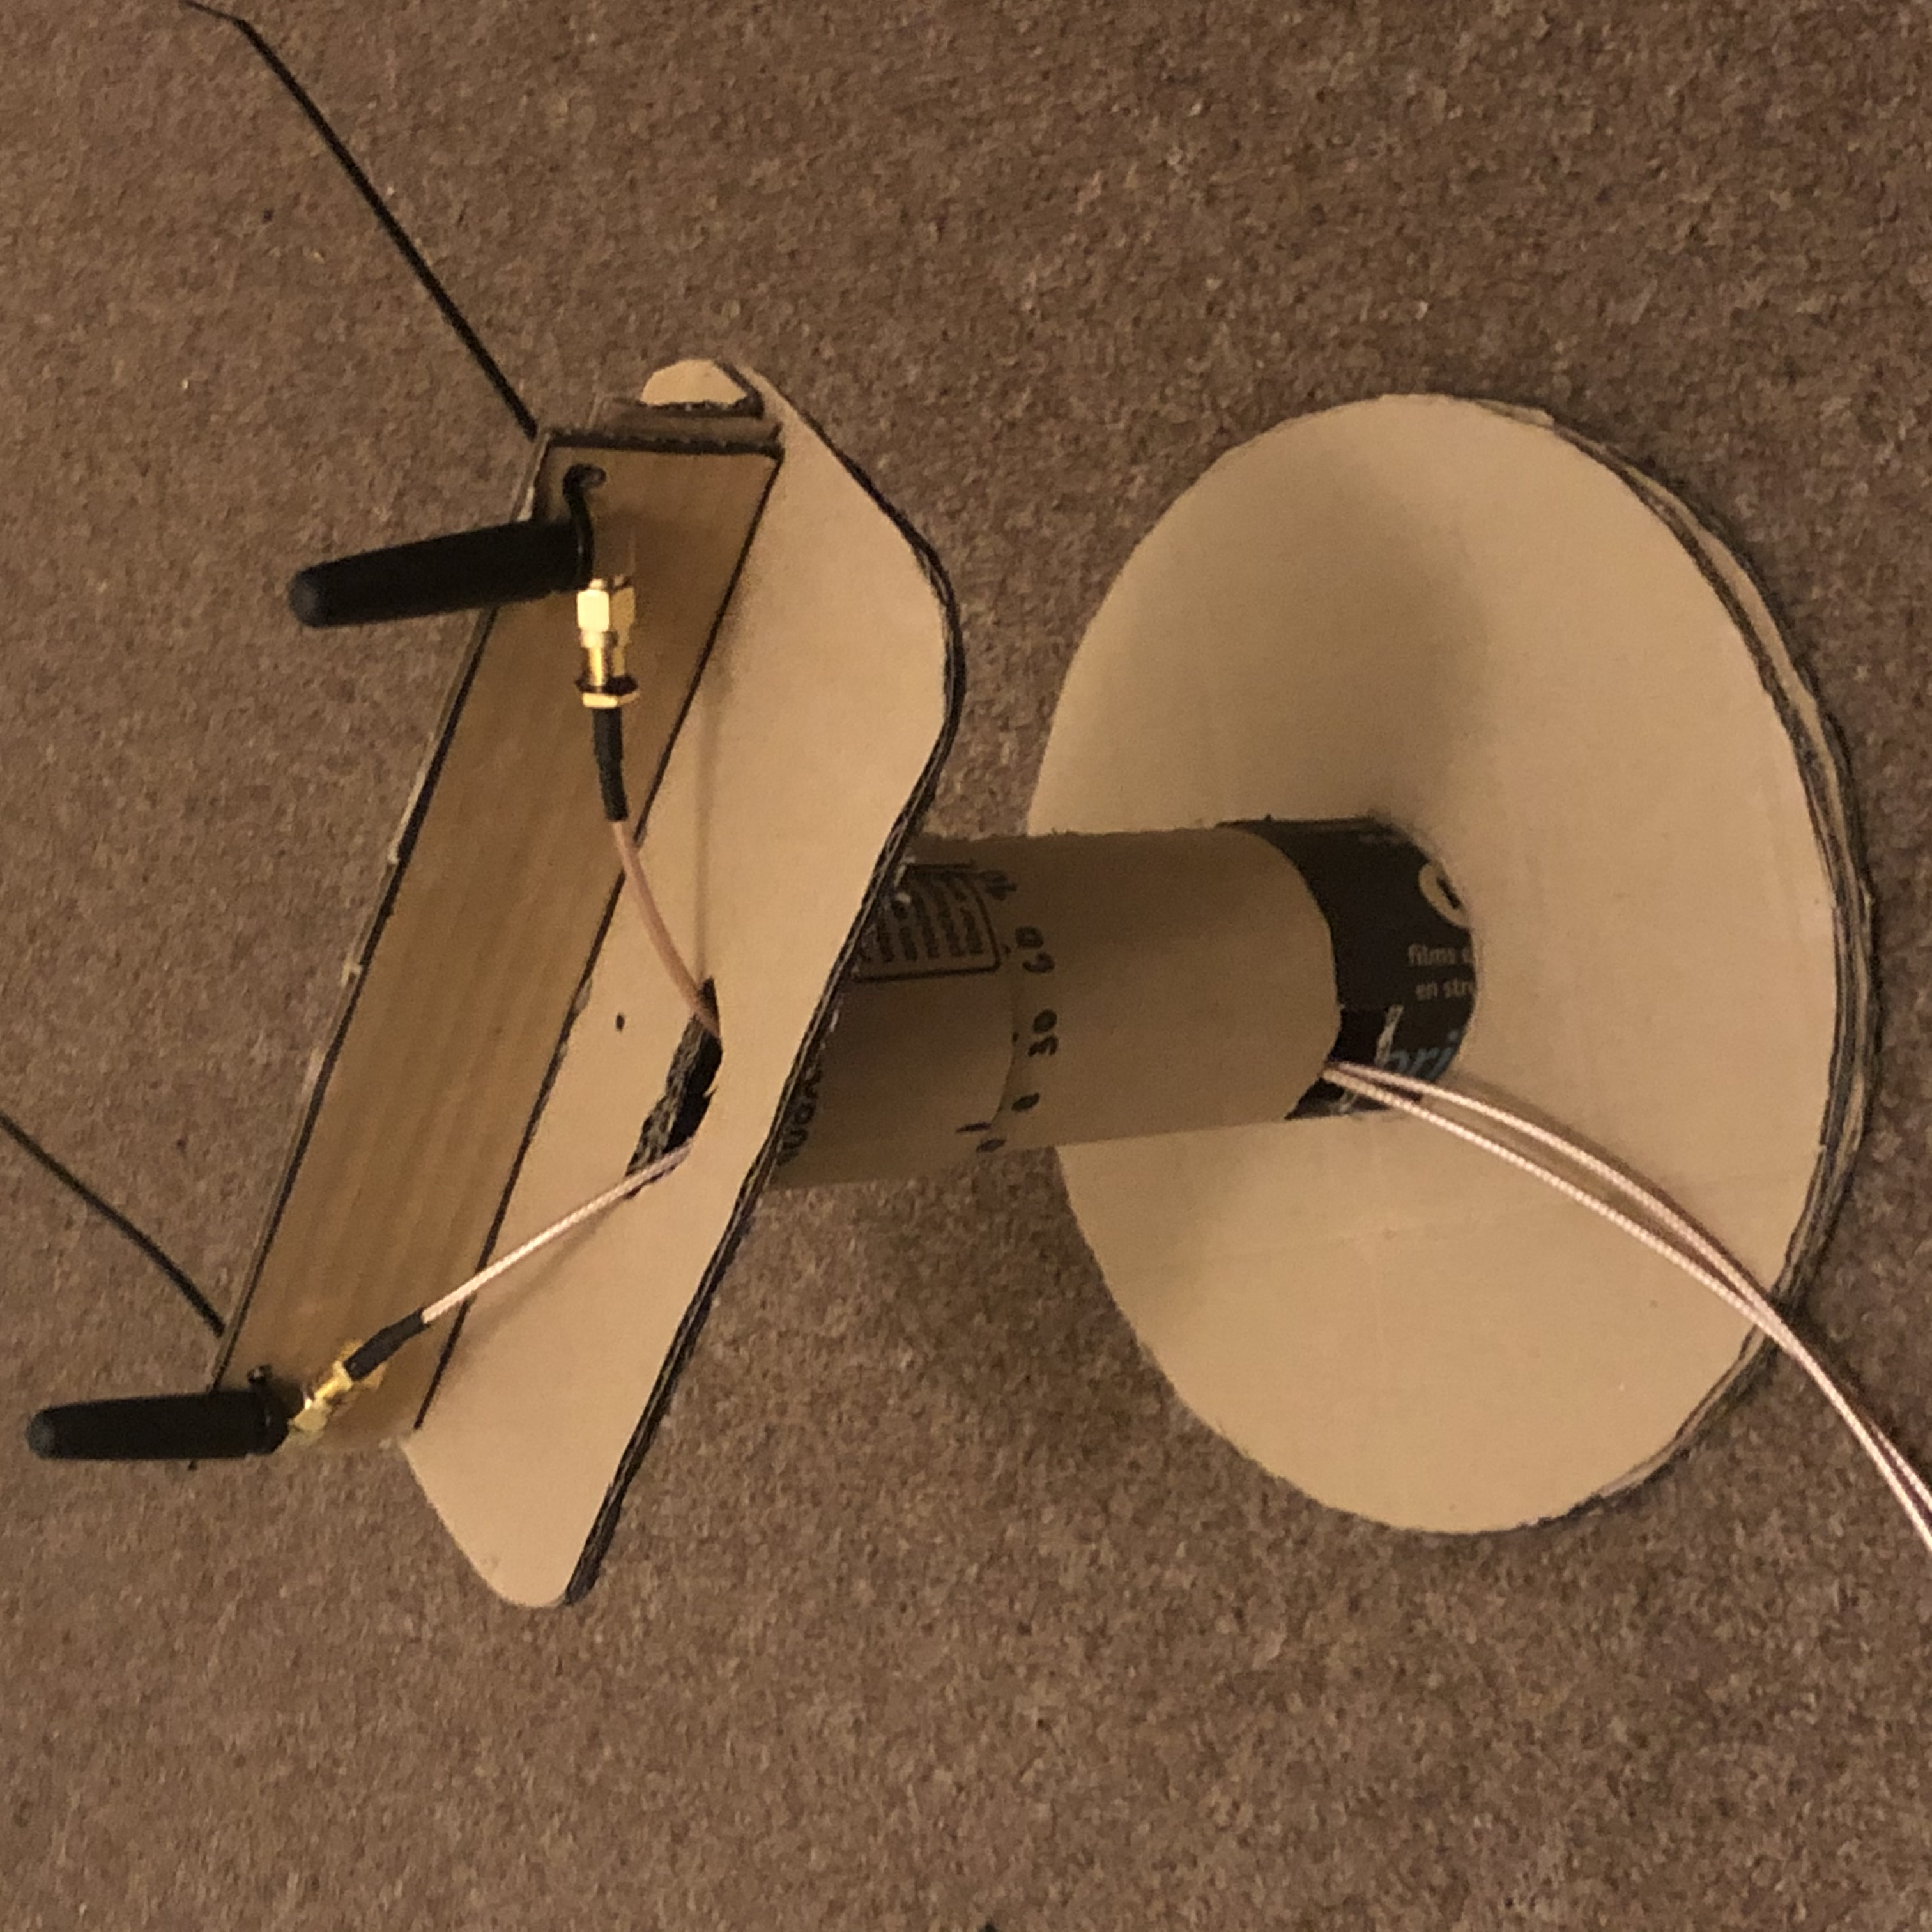
\includegraphics[width = 0.7\textwidth]{Figures/tb_real.jpg}
    \caption{Handmade antenna structure with antennas and SMA cables.}
    \label{fig:tb_real}
\end{figure}

\begin{figure}[!]
    \centering
    \begin{subfigure}{0.4\textwidth}
        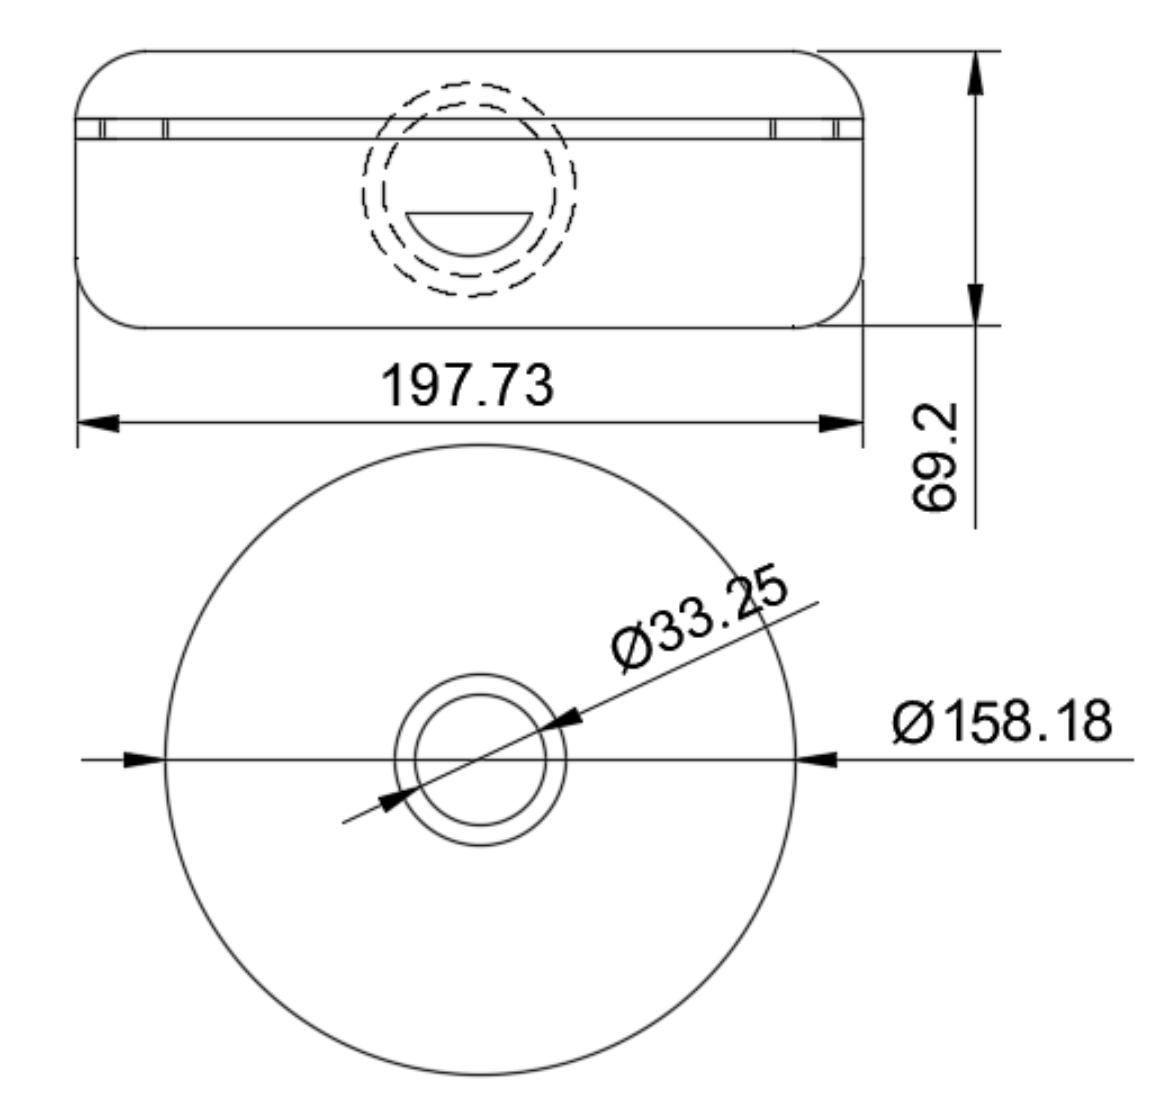
\includegraphics[width = \textwidth]{Figures/tb_top.png}
        \caption{Top view.}
    \end{subfigure}
    \begin{subfigure}{0.4\textwidth}
        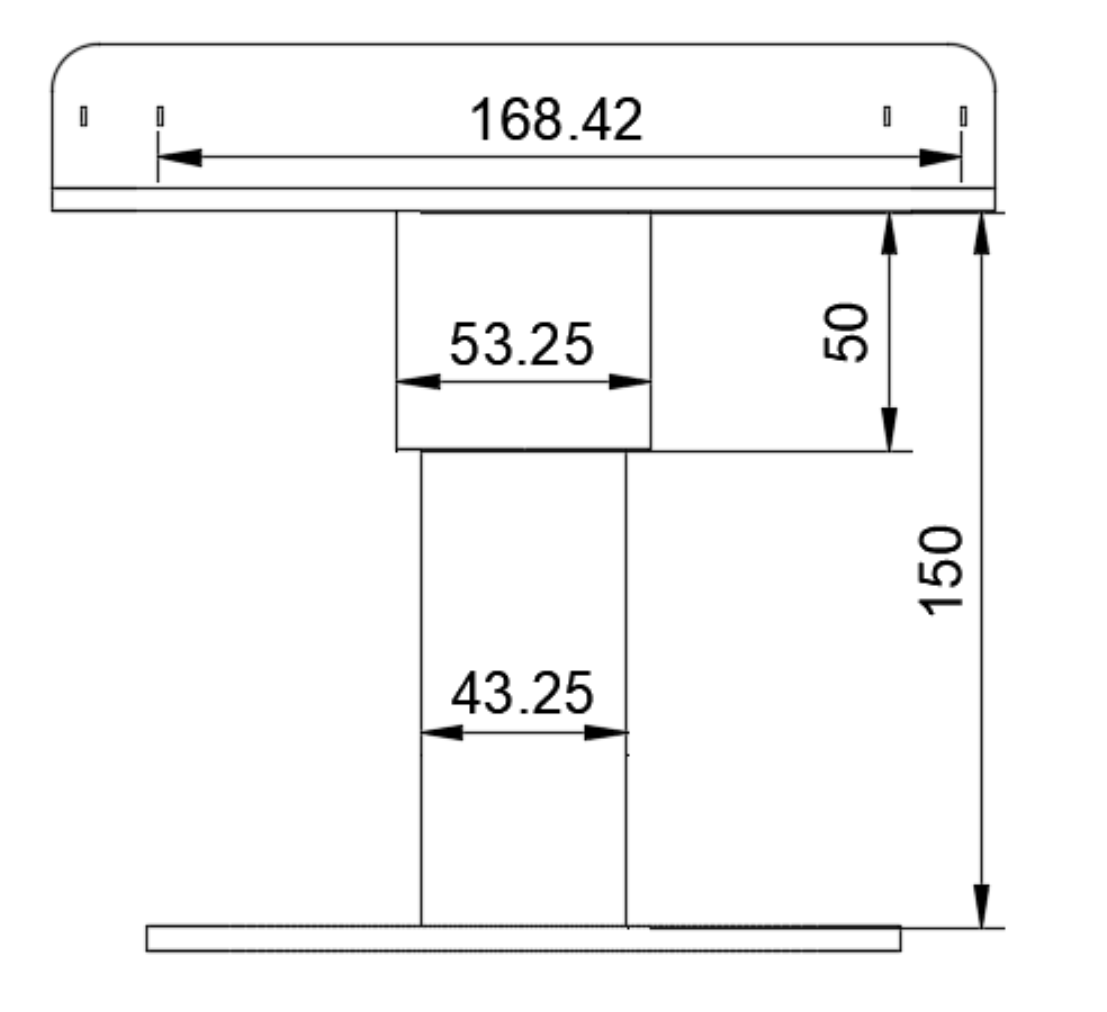
\includegraphics[width = \textwidth]{Figures/tb_front.png}
        \caption{Front view.}
    \end{subfigure}
    \caption[Technical drawing of the antenna holder.]{Technical drawing of the antenna structure considering $f_c = 890$ MHz and $M = 2$.}
    \label{fig:tb_draw}
\end{figure}

\newpage
\section{Hardware-in-the-Loop Demonstration} \label{met:hil}
The HIL demo is the combination of all the previous sections to have a template model to test individual components and further develop the UE tracker, similar to the simulation. The demo consists of transmitting and receiving a fixed frame using the BladeRF. The same subsystems used to develop the simulation in Section \ref{met:sim} were used in this section for modulating, receiving and to process the beamforming algorithm. The model resembles the one shown in figure \ref{fig:sim}, only lacking the DOA estimator at the BS, as adding it would require an additional antenna array and a SDR unit. 

The user can input the DOD at the transmitting end and the DOA at the receiver or use a function similar to the one for the UE movement in section \ref{met:problem}; and even change it from one to the other in run time. The DOA at the receiver side is estimated using the same algorithm as in the simulation, and the user can select whether to input the steering angle manually or to use the measured DOA; again, that can be alternated at run time. Some performance metrics, such as the BER and Error Vector Magnitude (EVM) and the RMS power of the beamformed signal, are logged to check the system's performance.

\begin{figure}[h]
    \centering
    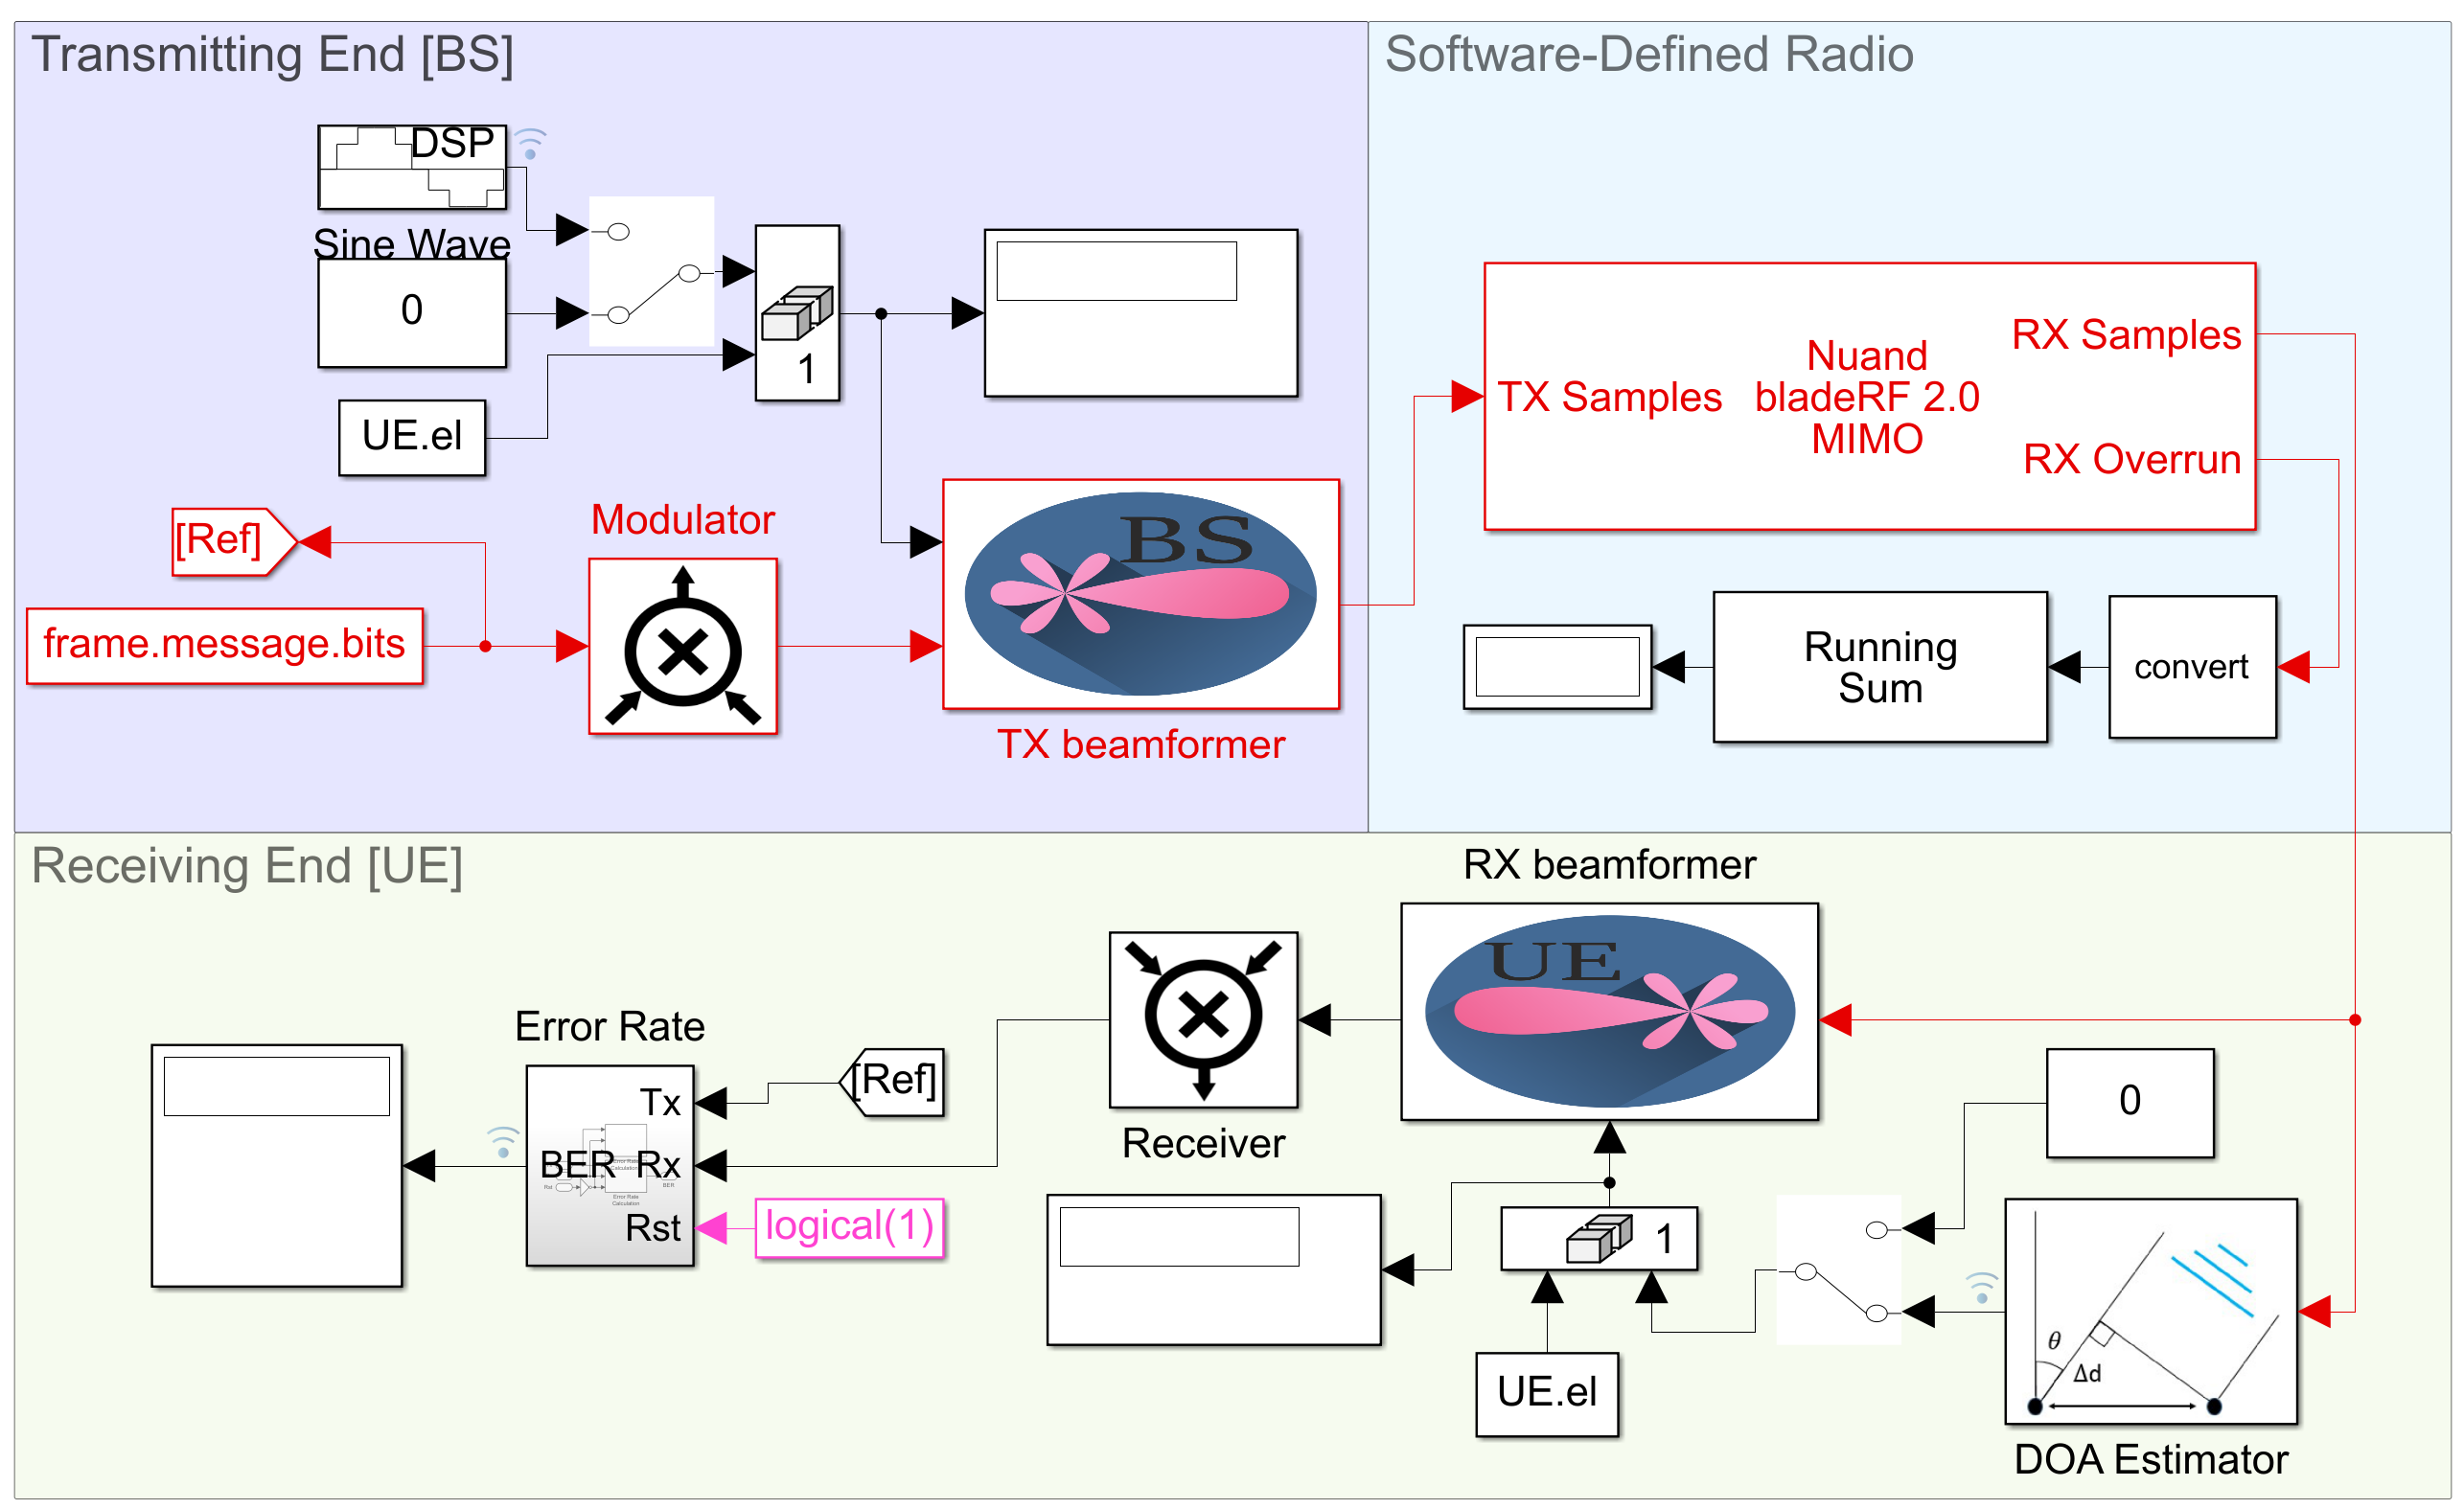
\includegraphics[width = \textwidth]{Figures/hil_demo.png}
    \caption{Simulink model for the HIL demonstration.}
    \label{fig:hil_demo}
\end{figure}

\chapter{Tests and Validation} \label{test}

\section{Introduction} \label{test:intro}
This section describes the tests and validation methods used to evaluate the products of chapter \ref{met}. Each subsystem of the system had to be tested to guarantee the system's performance, and the testing process for each is unique in order to show its strengths and weaknesses.

The tested parts are the products of sections \ref{met:sim:mod}, \ref{met:sim:bf}, \ref{met:int:mat}, the end-to-end simulation described in section \ref{met:sim} and several variations if the HIL demo in section \ref{met:hil}. As expected, the beamforming related tests are prioritised, as the remaining subsystems are evaluated to diagnose any discrepancy at the end-to-end simulation and real test.

Most of the variables used on for the tests are constrained by the SDR parameters and the antenna structure, resulting in the testing parameters shown in table \ref{tab:parameters:general}.

\begin{table}[h]
    \centering
    \begin{tabular}{c|c}
        Parameter &  Value\\ \hline
        Simulation step time ($T_s$) & 0.01 s \\
        Carrier frequency ($f_c$) & 890 MHz \\
        Number of antennas ($M$) & 2 \\
        Baseband sample rate ($f_{bb}$) & 1 MSPS \\
        Samples per simulation step ($N_{s/s}$) & 10000 \\
        Number of message bits ($N_m$) & 160 \\
        Number of preamble bits ($N_p$) & 40 \\
    \end{tabular}
    \caption{System parameters for the test scenarios.}
    \label{tab:parameters:general}
\end{table}

\newpage
\section{MIMO Interface for the BladeRF} \label{test:sdr}
The effort presented in section \ref{met:int} refers to a MATLAB interface for using the 2x2 MIMO scheme of the BladeRF SDR. This interface is used in the following sections as the real-world performance test; hence, its performance must be confirmed to be as expected. 

The test environment for the SDR is simple. The SDR is meant to capture the signal coming from an FM radio station and re-transmit it into an empty portion of the ISM band. The goal of the re-transmission is to validate both the TX and RX stages of the MATLAB interface. The validation metric for this test is to reproduce the signal coming from the BladeRF using another SDR; the test is considered valid if the audio signal is reproduced without artefacts consequence of dropout or discontinuities. Discontinuities may be caused by incorrectly interleaving the TX buffer or de-interleaving the RX buffer, having a high sample rate that affects determinism, having a large RX gain or an incorrect AGC setting. Also, the frequency spectrum of both signals can show if any discrepancy happened during the transmission. The Simulink model used for this test is shown in figure \ref{fig:test:sdr}, and consists of the \verb|bladeRF_MIMO| Simulink block in a feedback loop. The signal sensed by the second SDR is processed separately using the SDR Console console software. The RX and TX frequencies for the SDR are 92.32 MHz and 890 MHz, respectively.

\begin{figure}[h]
    \centering
    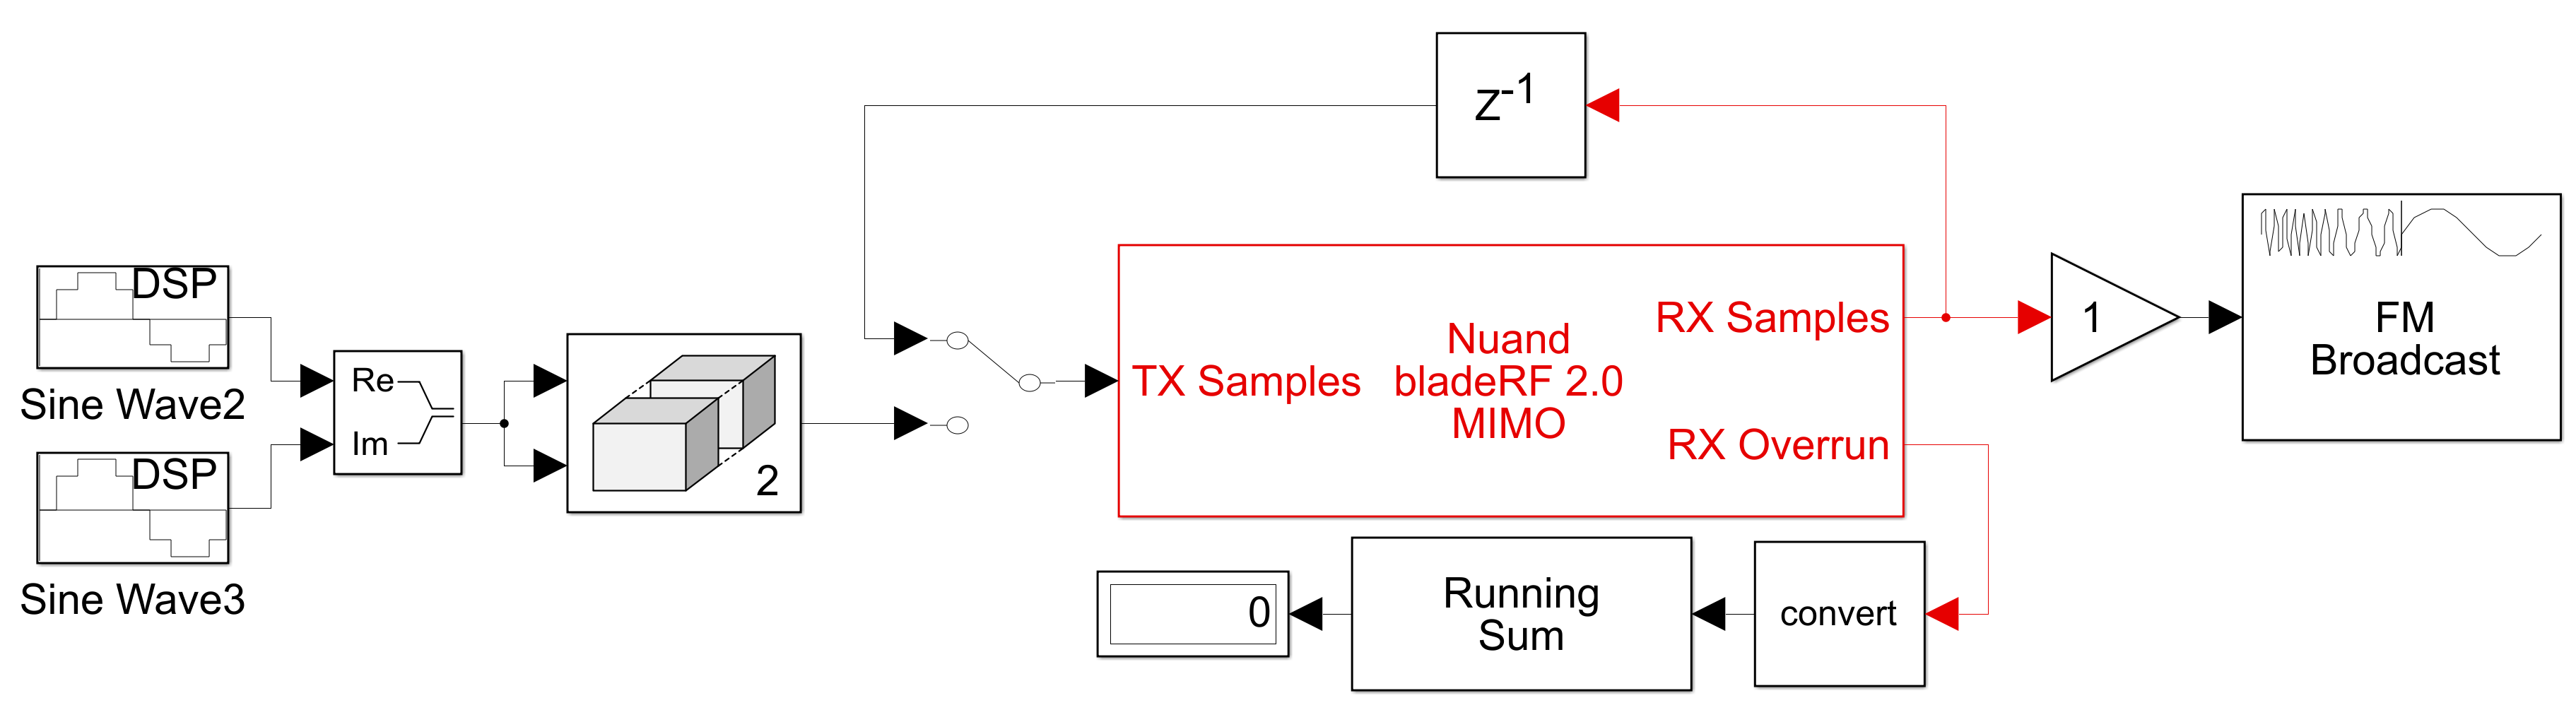
\includegraphics[width = \textwidth]{Figures/test_sdr.png}
    \caption{Simulink model for testing the MIMO interface of the BladeRF.}
    \label{fig:test:sdr}
\end{figure}

The first thing to consider is that the \verb|bladeRF_MIMO| block can transmit and receive coherent MIMO signals without dropping any sample. This feature was evaluated by adding the running sum block to the RX Overrun output, as this block evaluates whether some samples were dropped in the current time step as described in section \ref{met:int:lib:rx}. If the number in the display keeps increasing during run time, the system is not considered deterministic as the time step of the model is not constant. 

Figure \ref{fig:test:sdr:spectrum} shows the frequency spectrum of both signals. The signal received from the radio station is considered the baseline signal, and its meant to be compared to the signal received from the SDR; ideally, both spectrums should be identical. Often, artefacts in the time domain such as discontinuities are sensed as big spikes that sound similar to a short burst of white noise. These bursts are shown in the frequency domain as spikes in the mid-high end of the spectrum. However, the spectrum from the re-transmitted signal closely matches the reference as the main difference is that the re-transmission increases the noise-floor and presents a slightly more powerful response in the low-powered sections of the spectrum. Finally, no figure is presented for every channel layout as the results are very similar across channels.

\begin{figure}
    \centering
    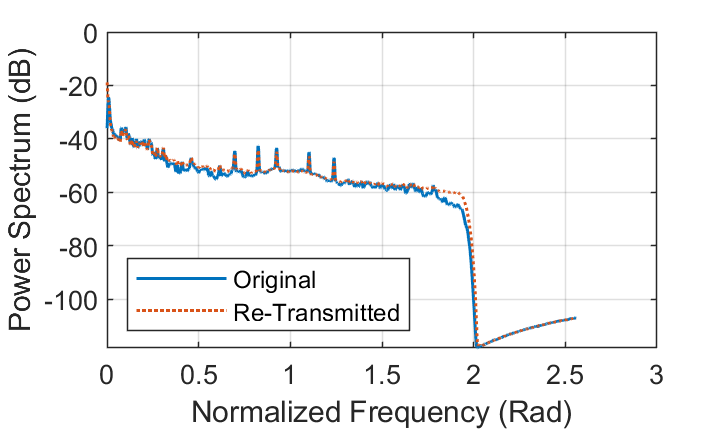
\includegraphics[width = 0.6\textwidth]{Figures/sdr_spectrum.png}
    \caption{Frequency spectrum of the signals coming from the radio station and the SDR.}
    \label{fig:test:sdr:spectrum}
\end{figure}

The second test scenario for the MIMO interface for the BladeRF is to receive a self-generated signal described in equation \ref{eq:test:sdr:iq}. The goal of this test if to visually inspect the received IQ signal from both receiver channels of the SDR. The expected result is two IQ signals with similar shape (given by equation \ref{eq:test:sdr:iq}) but phase-shifted, as the signal sensed by an antenna array delayed between antenna elements and this delay is represented by a phase shift. The actual phase shift is not essential for this test, as this is evaluated in section \ref{test:bf:rx:doa}.

Figure \ref{fig:test:sdr:iq} shows a constellation diagram containing the IQ signals from both RX channels in the SDR. The fading colour in both trails represents the signal's path in time. Although the signal's shape resembles equation \ref{eq:test:sdr:iq}, some artefacts can be found in some segments of the trail which are caused by the SDR's AGC trying to compensate the for the IQ imbalance in the IQ signal. Finally, signals from both channels RX0 and RX1 are close to orthogonal, confirming the expected output of two similar but phase-shifted signals.

\begin{equation}
    y(t) = I(t) + j Q(t) = \sin(2\pi (100) t) + j 0.6 \sin(2\pi(100) t + \frac{\pi}{2})
    \label{eq:test:sdr:iq}
\end{equation}

\begin{figure}[h]
    \centering
    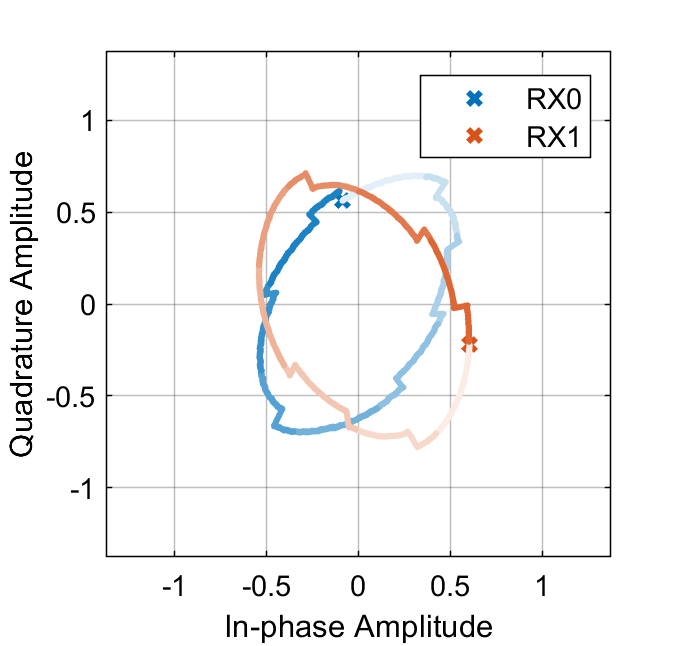
\includegraphics[width = 0.4\textwidth]{Figures/rx_channels.png}
    \caption{IQ signal from both RX channels in the SDR.}
    \label{fig:test:sdr:iq}
\end{figure}

\section{Modulator and Receiver} \label{test:mod_rec}
This section evaluates both modulator and receiver blocks as if they were part of a non-beamformed communications system. The overall simulation parameters are as the ones given in table \ref{tab:parameters:general} and the goal is to simulate a reliable end-to-end communication system using an SDR. The simulation will include some channel impairments such as Gaussian noise and a complex phase shift; the latter is essential as the TX and RX LOs in the SDR will cause a phase shift in the received symbols. Other parameters and details are not reviewed in this simulation as these blocks are not the main topic of this report. 

\begin{figure}[h]
    \centering
    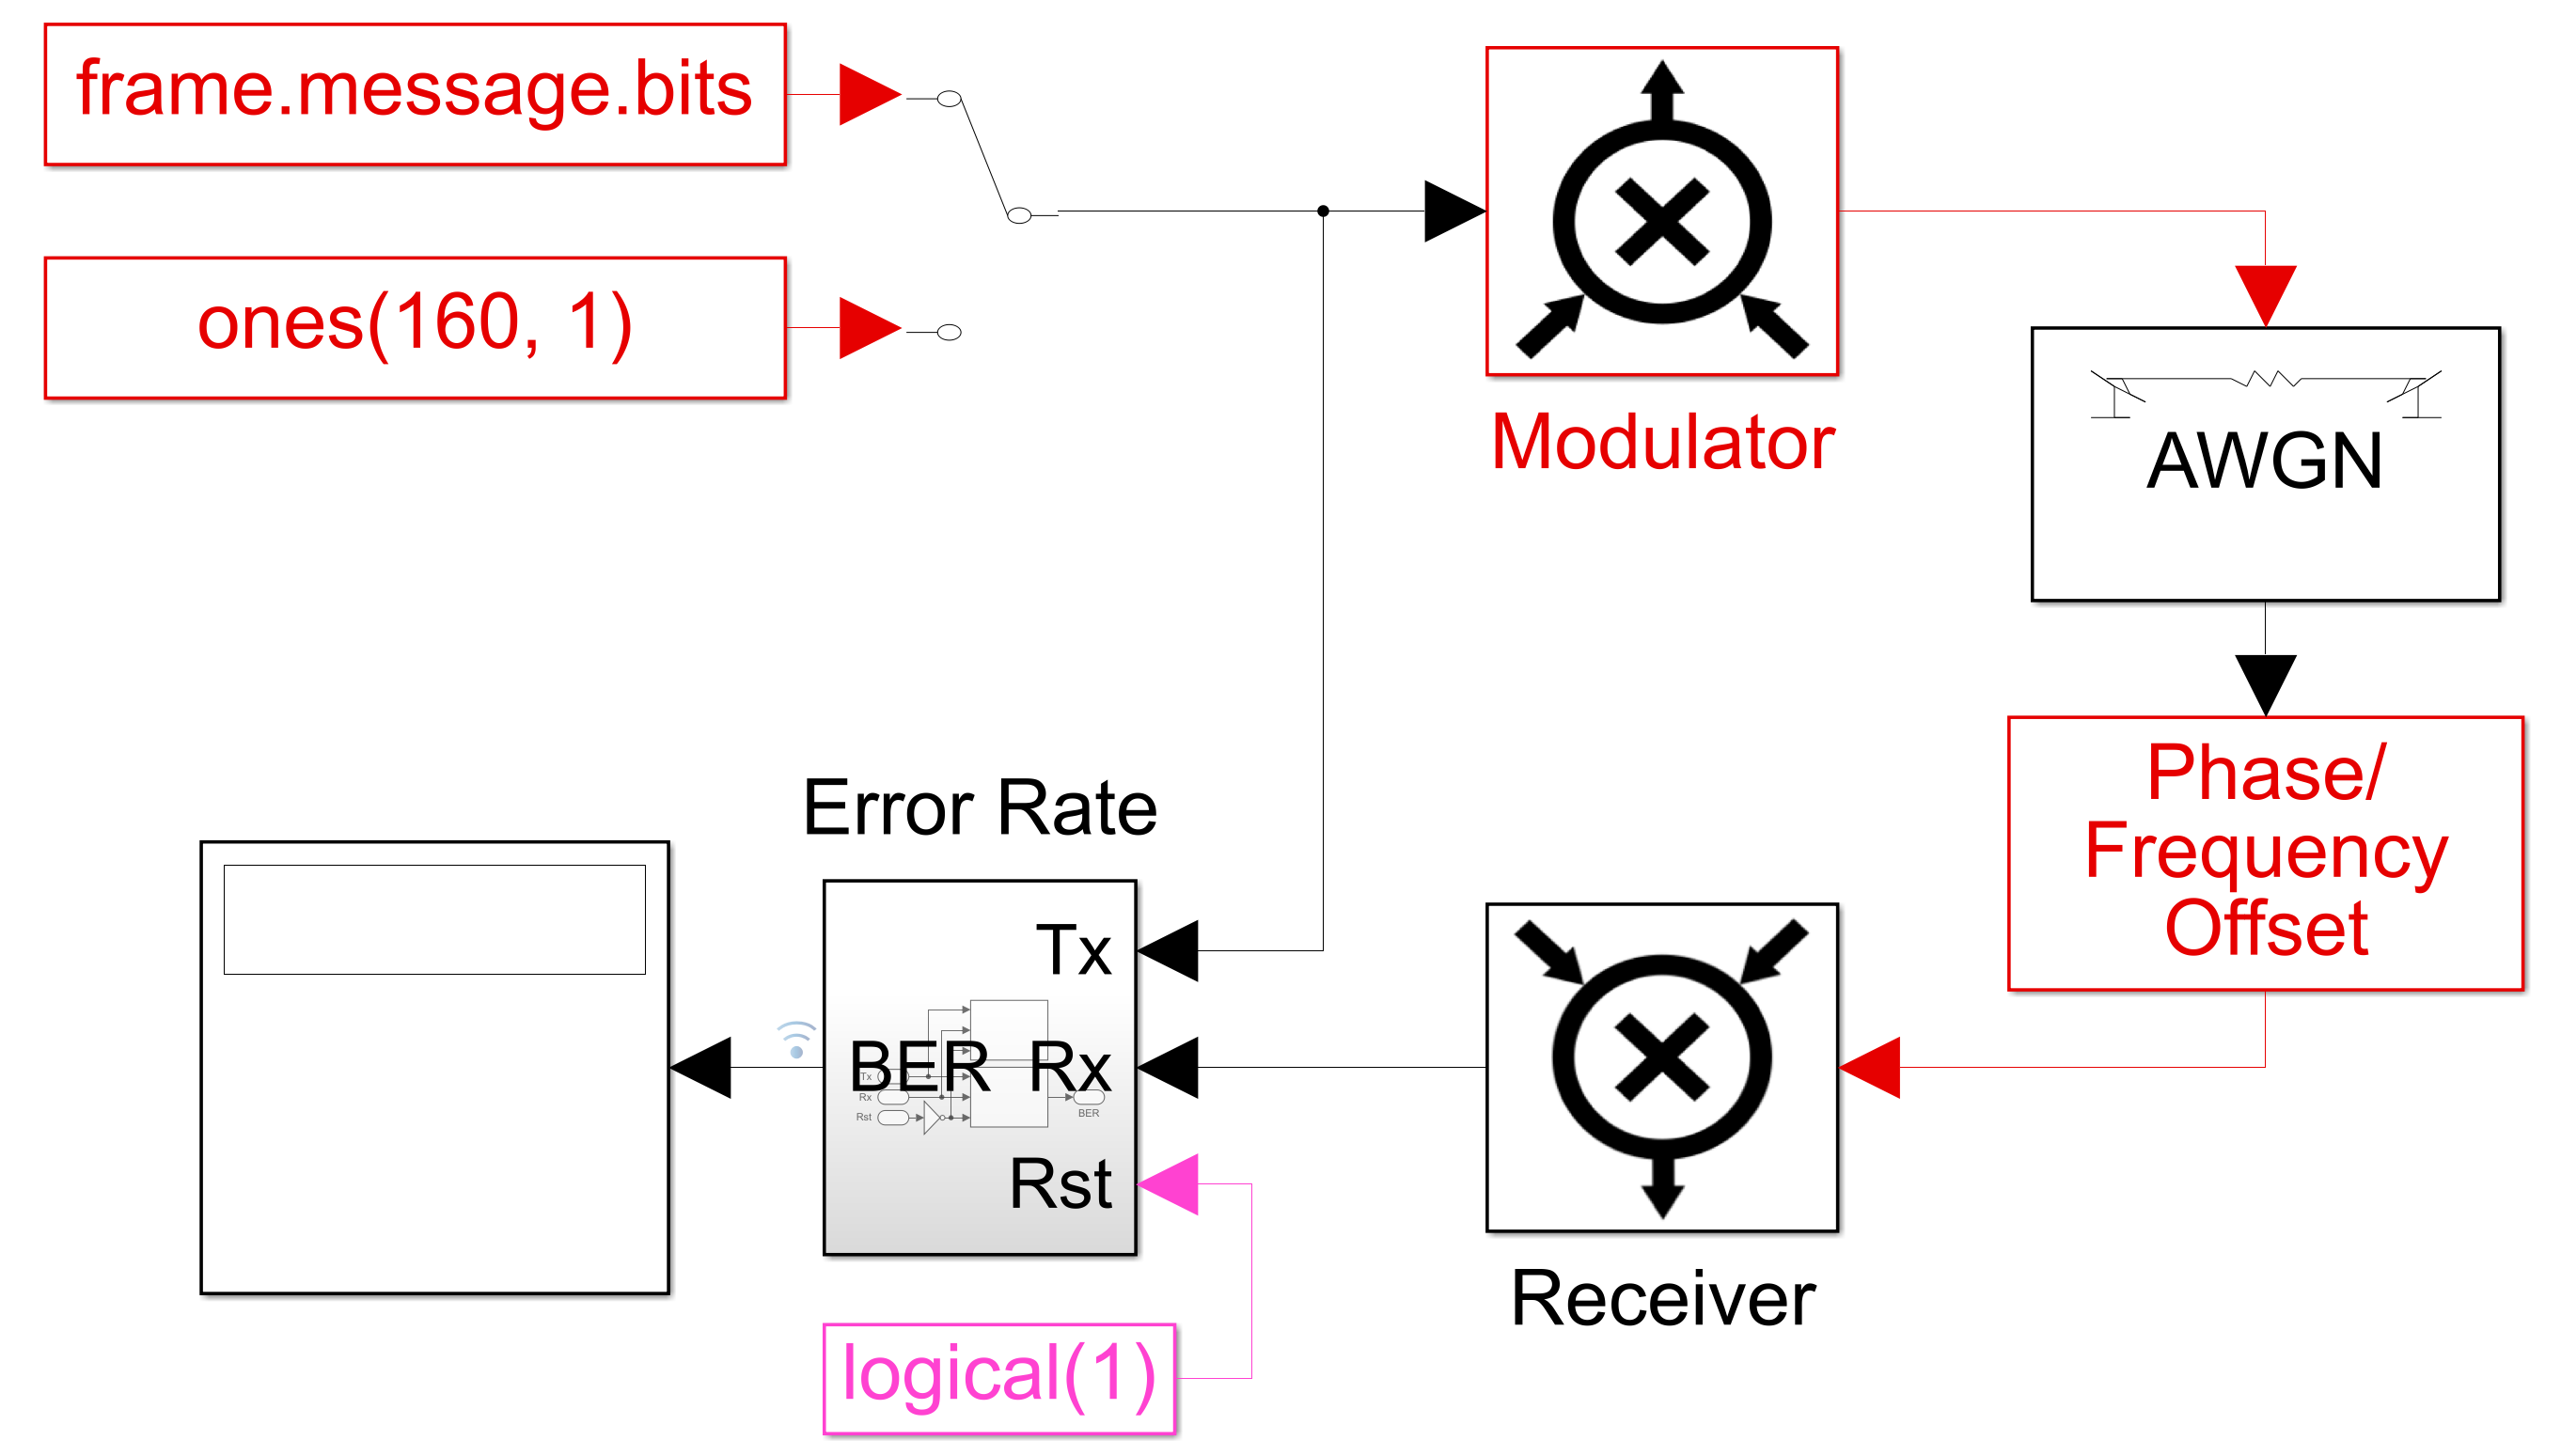
\includegraphics[width = 0.6\textwidth]{Figures/test_mod_rec.png}
    \caption{Simulink model for testing the Modulator and Receiver blocks.}
    \label{fig:test:mod_rec}
\end{figure}

\subsection{Modulator} \label{test:mod_rec:mod}
Since the modulator block is considerably less complicated than the receiver block, its analysis is reduced to a constellation diagram showing the output of a constant sequence of ones as bit input, as its best metric is an end-to-end simulation which is reviewed in the next section. This sequence is used as input because the modulator must be able to spread the bits into several different symbols before interpolation. The expected output is a complex IQ signal with a few deviations from the reference constellation, as the roll-off coefficient of the Raised Cosine filter is less than 1.

Figure \ref{fig:test:mod_rec:mod_iq:ones} shows the output of the modulator block when given a constant one sequence. The signal is 10,000 samples long, and it shows curved paths, a consequence of the roll-off coefficient. The signal features every possible symbol from the reference constellation disregarding the constant nature of the input sequence. 

\begin{table}[h]
    \centering
    \begin{tabular}{c|c}
        Parameter & Value \\ \hline
        Scrambler: Polynomial & $1 + z^{-1} + z^{-2} + z^{-4}$ \\
        Scrambler: Initial Condition & 0 0 0 0 \\
        \hline
        Raised Cosine: Roll-off & 0.3 \\
        Raised Cosine: Filter Span & 6 \\
        Raised Cosine: Interpolation Factor ($N_{int}$) & 100 \\
        Raised Cosine: Linear Amplitude Gain & $\sqrt{100}$ \\
    \end{tabular}
    \caption{Testing parameters for the modulator block.}
    \label{tab:parameters:modulator}
\end{table}

\begin{figure}[!h]
    \centering
    \begin{subfigure}{0.4\textwidth}
        \centering
        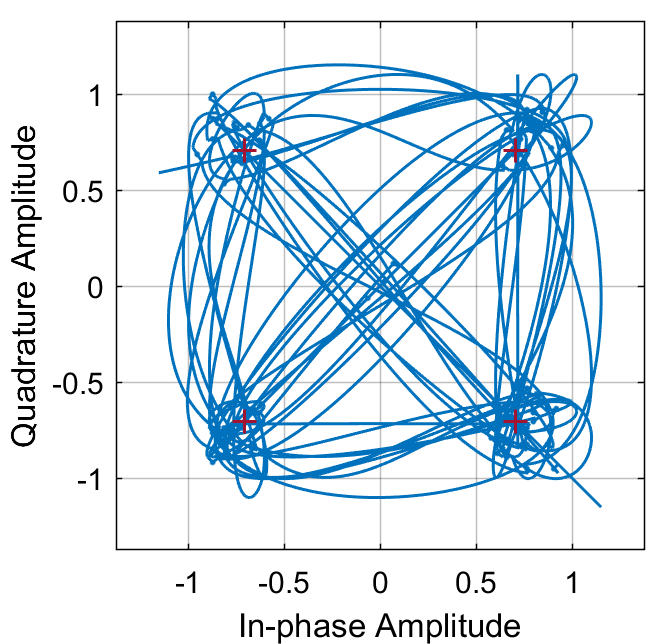
\includegraphics[width = \textwidth]{Figures/mod_frame.png}
        \caption{IQ signal for the default message bits.}
        \label{fig:test:mod_rec:mod_iq:frame}
    \end{subfigure}
    \hspace{0.1\textwidth}
    \begin{subfigure}{0.4\textwidth}
        \centering
        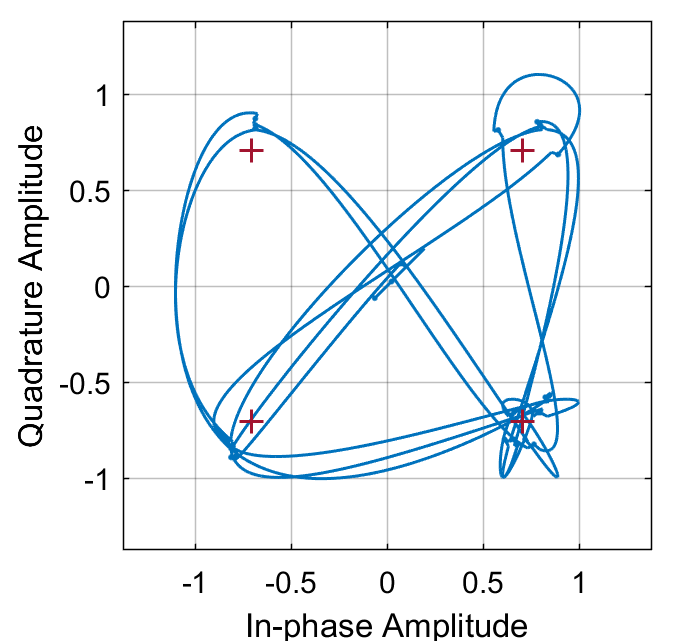
\includegraphics[width = \textwidth]{Figures/mod_ones.png}
        \caption{IQ signal for the constant bit sequence.}
        \label{fig:test:mod_rec:mod_iq:ones}
    \end{subfigure}
    \caption{Constellation diagrams showing different modulated signals.}
    \label{fig:test:mod_rec:mod_iq}
\end{figure}

\subsection{Receiver} \label{test:mod_rec:rec}
The receiver is one of the most complex algorithms that were developed for this work. As described in section \ref{met:sim:mod:rec}, it samples, synchronises, corrects and demodulate the input signal in order to get the same frame bits as the ones transmitted. The used validation metrics for this block are the elapsed time for the carrier synchroniser to reach the steady-state and the BER. The tests were done assuming a critically dampened synchronizer $\zeta_{cs} = 1$.

\begin{table}[!h]
    \centering
    \begin{tabular}{c|c}
        Parameter &  Value\\ \hline
        Raised Cosine: roll-off ($\beta$) & 0.3 \\
        Raised Cosine: filter span & 6 \\
        Raised Cosine: Decimation Factor ($N_{dec}$) & 10 \\
        \hline
        AGC: Time step & 0.01 s\\
        AGC: Output power & 1 W \\
        AGC: Average Length & 100 \\
        \hline
        Carrier Synchronisation: Samples per symbol & 10 \\
        Carrier Synchronisation: Damping factor ($\zeta_{cs}$)& 1 \\
        \hline
        Symbol Synchronisation: Samples per symbol & 10 \\
        Symbol Synchronisation: Damping factor ($\zeta_{ss})$ & 1 \\
        \hline
        Preamble Detector: Threshold & 14 \\
    \end{tabular}
    \caption{Testing parameters for the receiver block.}
    \label{tab:parameters:receiver}
\end{table}

Four simulation runs were logged using the parameters in \ref{tab:parameters:receiver} and different phase and noise values in order to test the overall performance of the receiver; the simulation time is 30 seconds. These parameters and the steady-state BER are shown in table \ref{tab:test:rec:test_params}. Also, an ideal baseline run is included.

\begin{table}[h]
    \centering
    \begin{tabular}{c|c|c||c}
        Experiment Number & Eb/No (dB) & $\phi_{err}$ & BER \\ \hline
        Baseline & Noiseless & 0 & 0.000166 \\
        (Ex) 1 & 5 & $20^\circ$   & 0.026124 \\ 
        (Ex) 2 & 5 & $130^\circ$  & 0.027701 \\
        (Ex) 3 & 20 & $20^\circ$  & 0.000299 \\
        (Ex) 4 & 20 & $130^\circ$ & 0.000845
    \end{tabular}
    \caption{Results of the receiver test scenario.}
    \label{tab:test:rec:test_params}
\end{table}

The simulations show that a more massive phase shift in the transmitted symbols results in a more extensive steady-state transient time for the carrier synchronisation, as shown in figure \ref{fig:test:rec:phase}. The transient time constraints the system's performance as the phase corrector is heavily impacted by the phase offset after the carrier synchronisation, resulting in erratic samples at the first few simulation steps. These outlier samples are always introduced by the synchronisation, affecting the steady-state BER. 

Although the carrier synchronisation needs some time steps to stabilise, for experiments three and four, the initial steady-state error was the only source of error on the communication system. As shown in figure \ref{fig:test:rec:ber_time}, the BER in experiments 1 and 2 is mostly affected by the low EbNo as it converges from the initial stabilisation-error to the expected BER shown in figure \ref{fig:test:rec:ber_snr}. However, the only errors in experiments 3 and 4 are the stabilisation errors, and no other artefacts were found in the simulation time.

\begin{figure}
\centering
\begin{subfigure}{0.45\textwidth}
\centering
    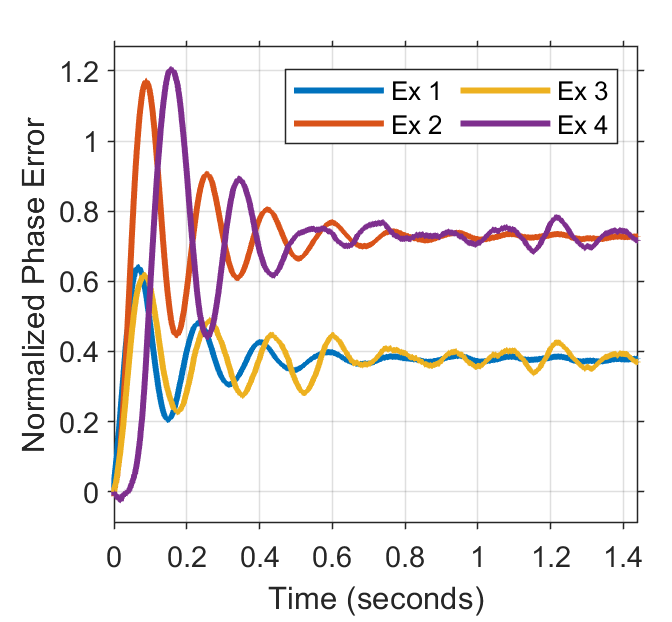
\includegraphics[width = \textwidth]{Figures/phaseerr_time.png}
    \caption[Phase error of the receiver tests.]{Normalised phase error from the carrier synchronisation for the test simulations.}
    \label{fig:test:rec:phase}
\end{subfigure}
\hspace{0.05\textwidth}
\begin{subfigure}{0.45\textwidth}
\centering
    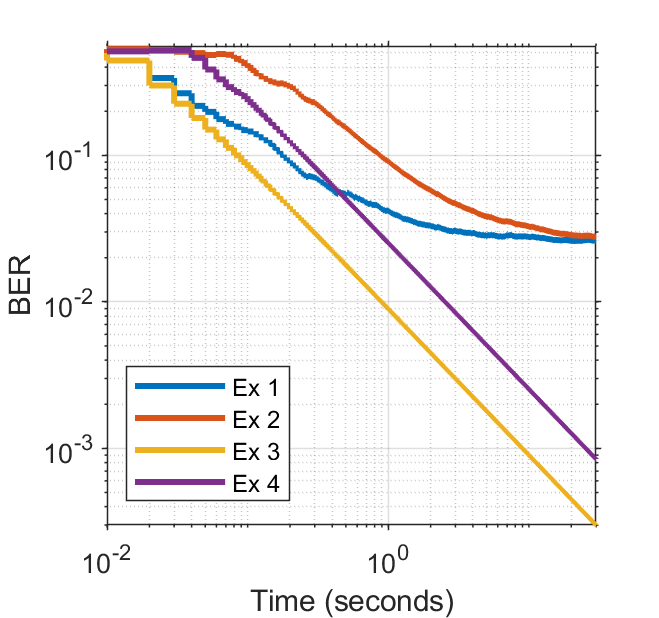
\includegraphics[width = \textwidth]{Figures/BER_Time.png}
    \caption[BER vs time of the receiver tests.]{BER across the simulation time for all simulations.}
    \label{fig:test:rec:ber_time}
\end{subfigure}
\caption[Results of the receiver test.]{Results for experiments in table \ref{tab:test:rec:test_params}.}
\end{figure}

The behaviour of the receiver in across Eb/No is expected, as the symbol synchronisation stage does affect the BER performance depending on the timing error, which is expected to be the performance bottleneck \cite{Mathworks2020SymbolSynchronization}. This simulation was also compared to the theoretical performance of QPSK in AWGN, and the result is shown in figure \ref{fig:test:rec:ber_snr}. The BER curve of the system with the receiver block reaches slightly worse error rates at the same Eb/No, compared to the system without the receiver block.

\begin{figure}[h]
    \centering
    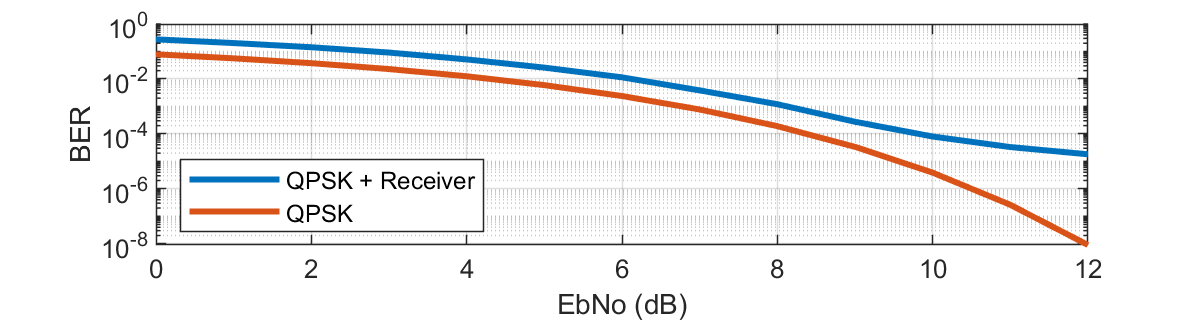
\includegraphics[width = 0.9\textwidth]{Figures/BER_EbNo.png}
    \caption[BER of the receiver test.]{BER across different Eb/No from the receiver subsystem simulation test. $\phi_{err} = 20^\circ$. The theoretical QPSK BER is compared to the simulation model using the Receiver subsystem.}
    \label{fig:test:rec:ber_snr}
\end{figure}

\newpage
\section{Beamformers} \label{test:bf}
Both phase-shift beamformers described in section \ref{back:bf:theoretical} and coded in section \ref{met:sim:bf} are subjected to different test to show whether they perform as expected. These tests are validated using the beamforming equations in section \ref{back:bf:theoretical}. 

\subsection{TX Beamformer}\label{test:bf:tx}
The testing in this section is meant to validate whether the TX beamformer emits a radiation pattern similar to the theoretical given in equation \ref{eq:combiner_freq3}. The test scenario consists on the TX antenna array being placed on an open area while a second SDR measures the received power from a signal transmitted by the beamformed array at different observation points ($O_m$) around the array. The distance $d_O$ from the array to $O_m$ must be constant, to maintain path loss consistent between experiments.

\begin{figure}[h]
    \centering
    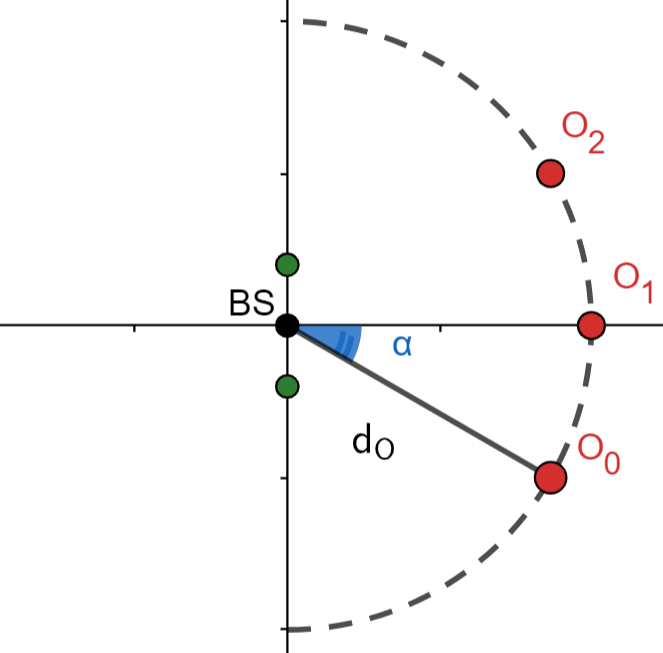
\includegraphics[width = 0.3\textwidth]{Figures/test_bf_tx.png}
    \caption[Example layout for the TX beamformer test.]{Location layout example for the TX beamformer test. The green dots are the antenna elements in the TX array, while $O_0$, $O_1$ and $O_2$ are different measurement locations around the array.}
    \label{fig:test:bf:tx}
\end{figure}

The Simulink model used for this test is the HIL demo in figure \ref{fig:hil_demo}, described in section \ref{met:hil}. Since only the TX beamformer was being evaluated, the components in the receiving end were excluded from the model.
The logged parameters of this experiments are the angle ($\alpha$) between $O_m$ and the $x$ axis of the antenna array, and the RMS power of the signals received at $O_m$. The validation metric for this experiment is a comparison of the theoretical radiation pattern and the logged RMS value. Both theoretical and received samples must be normalised in order to be comparable, as the theoretical plot represents the array gain, and the real samples do include the path loss attenuation. The normalisation is done using MATLAB's \verb| normalise | function and the z-score method that sets the output sequence's mean to zero and the standard deviation to one.

The coherency of the TX channels in the SDR can be evaluated using the previous methodology, but the beamforming algorithm is tested by steering the main beam and get the peak RMS value at a location different than $0^\circ$. The steering angle ($\phi$) present in equation \ref{eq:combiner_freq3} must be different than 0 degrees.

The actual test was carried out in a small garden, using a rope to establish a constant distance of $d_O = 2.2$ meters and a steering angle $\phi = 30^\circ$. The small size of the experiment area constrained access to the whole semi-circle around the array, limiting the number of data points. Finally, the SDR used to measure the RMS value must be configured to have a constant RX gain, instead of using the AGC.

\begin{table}[h]
    \centering
    \begin{tabular}{c|c|c||c}
        $\alpha$ & RMS($IQ(t)$) & Normalised & Theoretical\\ \hline
        $-50^\circ$ & 0.0017 & -0.3702 & -0.9080\\
        $-22^\circ$ & 0.0007 & -1.5273 & -1.681\\
        $0^\circ$ & 0.0022 & -0.2083 & 0.1994\\
        $22^\circ$ & 0.0029 & 1.0182 & 1.2060\\
        $50^\circ$ & 0.0026 & 0.6711 & 0.9603\\
    \end{tabular}
    \caption[Results of the TX beamforming test.]{Results for the measurements in $O_m$ at $d_O = 2.2$ meters and $\phi = 30^\circ$.}
    \label{tab:test:bf:tx}
\end{table}

Figure \ref{fig:test:bf:tx:pattern} contains the normalised theoretical radiation pattern, the normalised measurements from the real implementation and a second order interpolation of these measurements for improved visualisation. This figure shows that the interpolated plot greatly resembles the theoretical pattern. Overall, the measured pattern matches the theoretical better at the high-power section of the pattern (around $30^\circ$) than it does on the low-power section (around $-30^\circ$). This mismatch may be caused by the lack of observation points, the channel's noise or the phase-shift beamformer nature, as non-true time-delay beamformers tend to have un-sharp responses.

\begin{figure}[h]
    \centering
    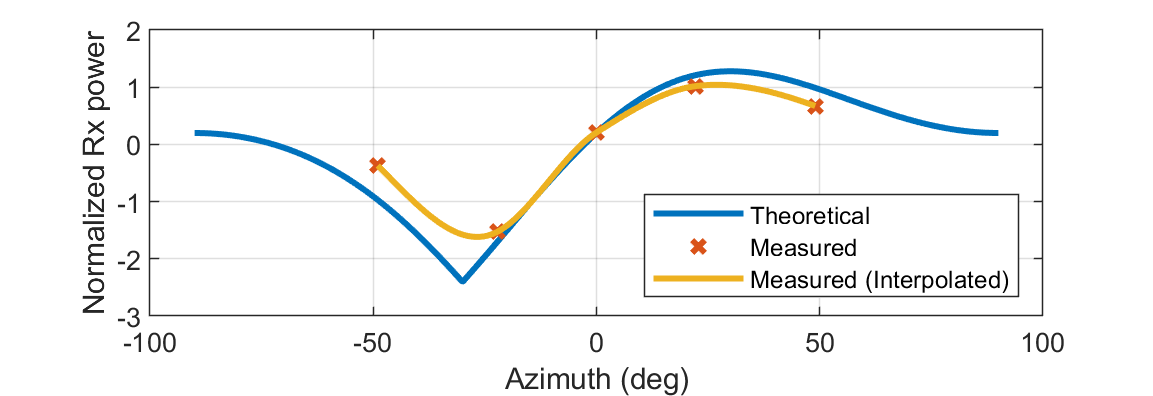
\includegraphics[width = 0.8\textwidth]{Figures/test_bf_tx_pattern.png}
    \caption[Normalised radiation patter for the theoretical and real beamformers.]{Normalised radiation patter for the theoretical and real beamformers. The measurements of the real implementation were interpolated to enhance its visualisation.}
    \label{fig:test:bf:tx:pattern}
\end{figure}

\subsection{RX Beamformer} \label{test:bf:rx}
The RX beamformer can also be considered interference rejecting as it can steer its main beam towards the desired signal's DOA and at the same time reject signal from sources coming from directions different to the desired. As stated in section \ref{back:bf:theoretical}, a beamformer can be modelled as a low-pass FIR filter, and the test environment for this block is meant to show the similarities of beamformers and digital filters. 

\subsubsection{Noise Rejection and Directivity} \label{test:bf:rx:noise}
The scenario consists of three elements, the RX antenna array, a wanted signal source ($S_{wan}$) and an interference signal source ($S_{int}$). The RX antenna array is placed on an open area, and both signal sources are placed at different locations making the DOA estimated by the antenna array significantly different. Ideally, this condition can be met by placing both devices at opposite ends of the array's coordinate system, but impairments as multipath results in electromagnetic waves refracting and bouncing into walls and other surfaces; hence, reaching the antenna array in unexpected directions. The goal for this test is to prove that the beamformer can attenuate a signal coming from un-wanted direction ($\theta_{int}$) while keeping the wanted signal by setting the beamformer's steering angle ($\phi$) to the wanted signal's DOA ($\theta_{wan}$); also the steering angle is set to a direction between $\theta_{wan}$ and $\theta_{int}$ to measure the beam's performance and sharpness, this direction is called $\theta_{null}$. 

\begin{figure}[h]
    \centering
    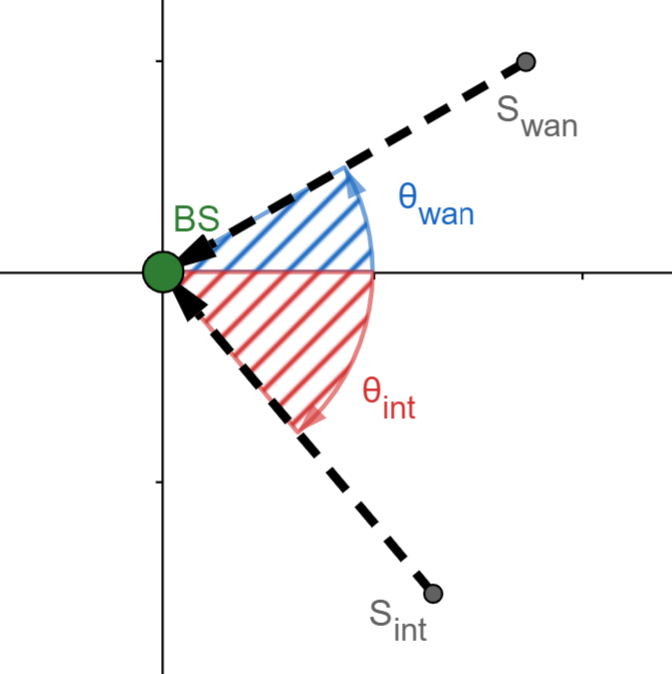
\includegraphics[width = 0.3\textwidth]{Figures/test_bf_rx.png}
    \caption[Example layout for the RX beamformer test.]{DOA layout example for the RX beamformer test. The wanted $S_{wan}$ and interference $S_{int}$ signal sources are arriving to the BS at different angles relative to the BS.}
    \label{fig:test:bf:rx}
\end{figure}

The metrics used for validation are the BER and EVM. The EVM outputs the resemblance of a signal to a reference constellation, considering phase, amplitude and noise variance. The EVM is based on the squared error between the measured and reference symbols. Hence, the lower the EVM, the greater the resemblance and performance \cite{Mathworks2020MeasureMagnitude}. The BER is used as an end-to-end performance metric and is expected to be lower when the beam is steered towards the wanted signal source. 

Two experiment sets are due, with and without the interference signal. The baseline run, without the interference, is meant to show the performance of the beamformer in terms of directivity. The actual test does include both signal sources. 

Both a simulation and real implementations were done for this scenario. Both consider the $\theta_{wan} = 25^\circ$, $\theta_{int} = -40^\circ$ and $\theta_{null}$, include the modulator and receiver block and the parameters given in tables \ref{tab:parameters:modulator} and \ref{tab:parameters:receiver}. The simulation also features channel impairments such as 10 dB SNR from an AWGN channel and $20^\circ$ phase offset.

The simulation model in figure \ref{fig:test:bf:rx:sim} consists of two signal sources, the wanted source comes from the modulator block, and the interference signal comes from a white noise source. The signal sensed by the RX antenna array is modelled as the superposition of both signals, described by equation \ref{eq:test:bf:rx:super}. The EVM calculation is done after the carrier synchronisation to discard the phase-shift introduced by the channel and beamformer, being the SNR the only impairment affecting the measurement.

The expected behaviour for this scenario is that BER and EVM improve as steering angle approaches the wanted signal's DOA. This trend is expected across the baseline and test runs, although the baseline runs may not present such an improvement, as the RX antenna array only contains two elements. As mentioned in \ref{back:bf:theoretical}, the number of elements in the array translates to the filter order of a low-pass FIR filter.

\begin{equation}
    y(t) = \sum^{M-1}_{m=0} (x_{wan}(t) + x_{int}(t) + n(t))w_m^* 
    \label{eq:test:bf:rx:super}
\end{equation}

\begin{figure}[h]
    \centering
    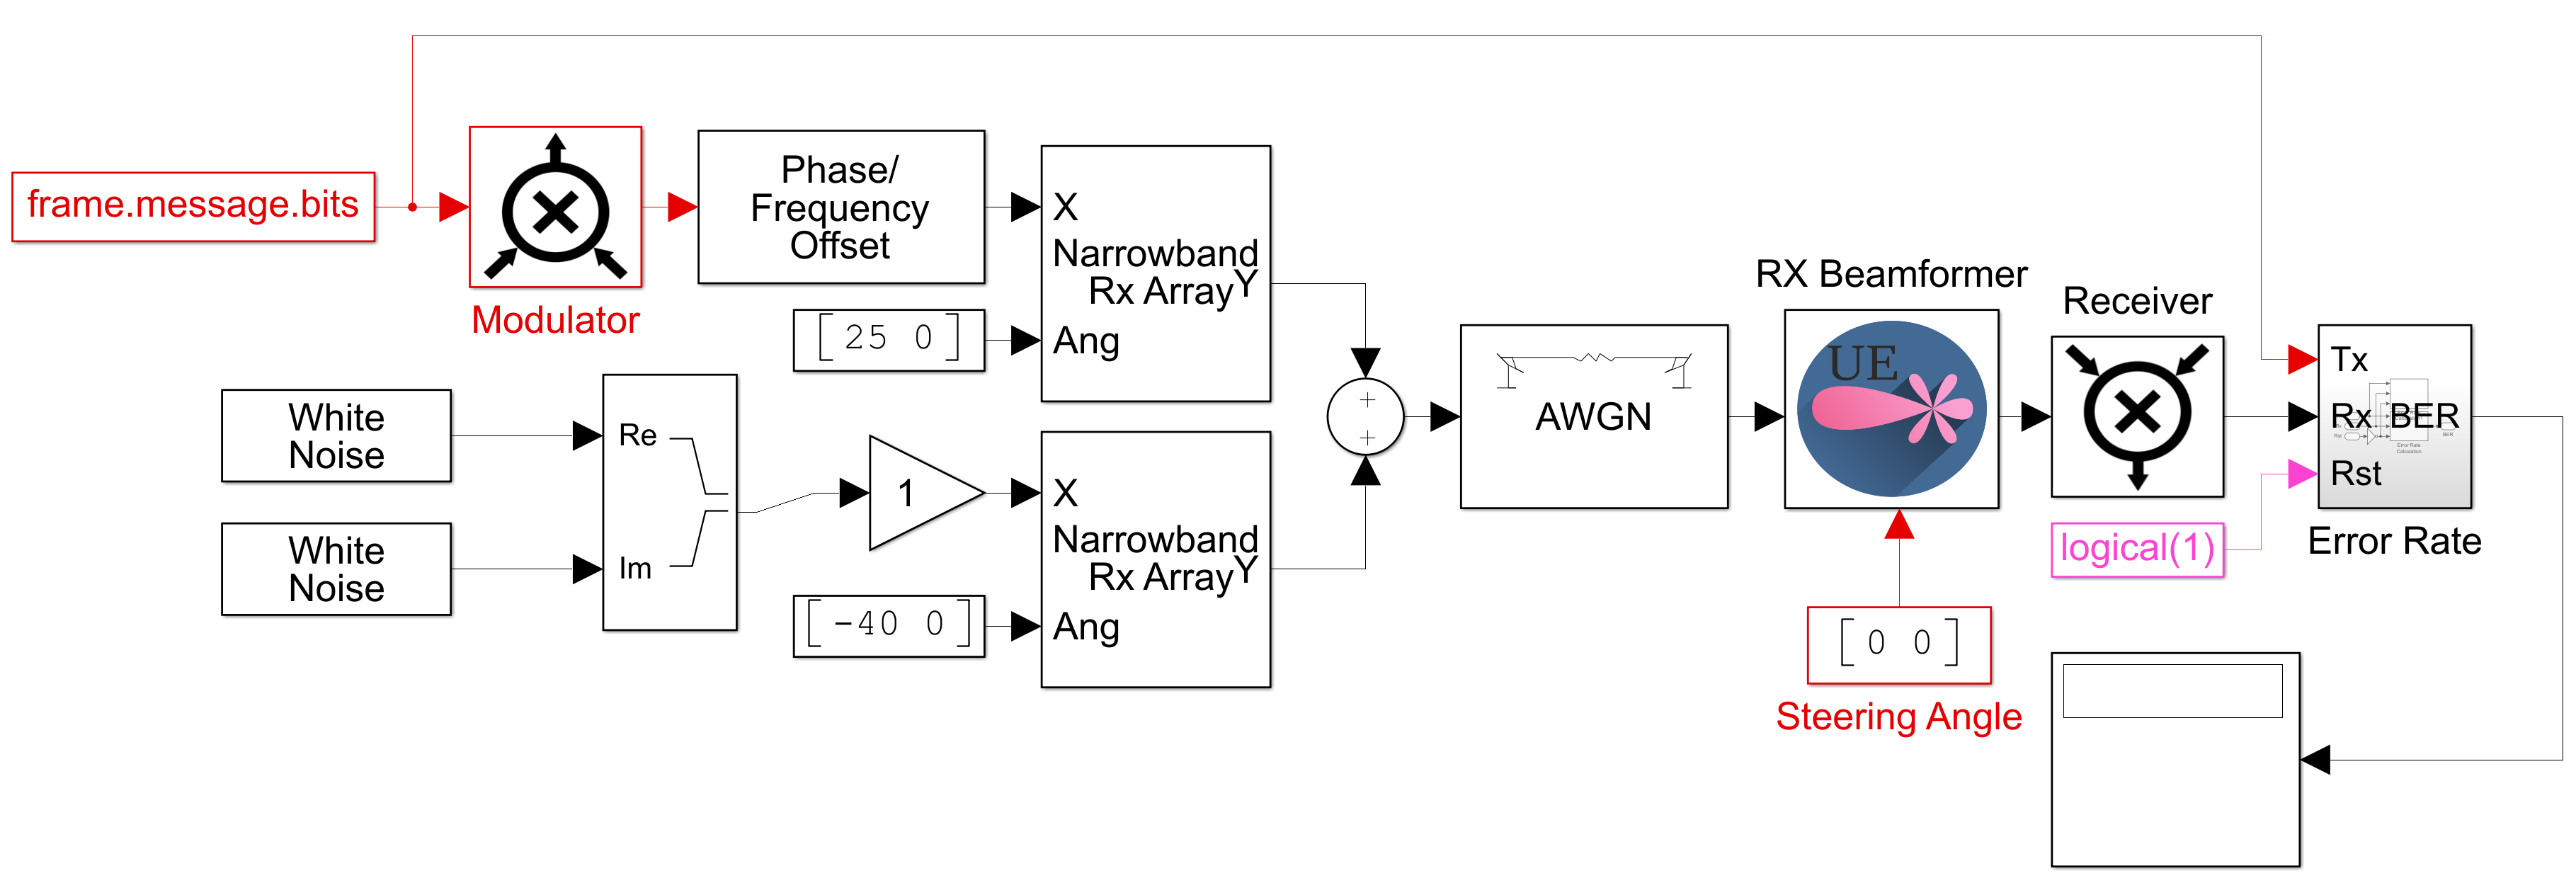
\includegraphics[width = \textwidth]{Figures/test_bf_rx_sim.png}
    \caption{Simulink model for representing the RX beamformer test scenario.}
    \label{fig:test:bf:rx:sim}
\end{figure}

The results for both simulation and real tests are shown in tables \ref{tab:test:bf:rx:test:sim}, \ref{tab:test:bf:rx:test:real}, \ref{tab:test:bf:rx:base:sim} and \ref{tab:test:bf:rx:base:real}. The baseline results in table \ref{tab:test:bf:rx:base:sim} show that, for a situation with a single signal source, the two-element beamformer is not completely filtering signals coming from $\phi \pm 25^\circ$; as the radiation pattern is wide enough for the AGC and carrier synchronizer to successfully recover the signals coming from $|\phi - \theta| < 25^\circ$, resulting in similar BER and EVM across the experiments with the steering angle set to $\theta_{wan}$ and $\theta_{null}$. The real scenario baseline run in table \ref{tab:test:bf:rx:base:real} shows less-ideal results but with the same trend as the simulations. 

\begin{table}[h]
    \centering
    \parbox{.45\linewidth}{
    \centering
    \begin{tabular}{c|c|c|c|c}
    & & \multicolumn{3}{c}{EVM (\%)} \\ 
    $\phi$ & BER & RMS & Max & 95th \\ \hline
    $\theta_{int}$ & 0.002891 & 47.62 & 87.19 & 79.06 \\
    $\theta_{null}$ & 0.000191 & 42.01 & 84.19 & 75.87 \\
    $\theta_{wan}$ & 0.000199 & 41.96 & 84.19 & 75.7
	
    \end{tabular}
    \caption[Simulated baseline results for the RX beamformer test.]{Baseline results from the simulated scenario.}
    \label{tab:test:bf:rx:base:sim}
    }
    \hfill
    \parbox{.45\linewidth}{
    \centering
    \begin{tabular}{c|c|c|c|c}
    & & \multicolumn{3}{c}{EVM (\%)} \\
    $\phi$ & BER & RMS & Max & 95th \\ \hline
    $\theta_{int}$ & 0.292900 & 51.68 & 86.85 & 88.69 \\
    $\theta_{null}$   & 0.002909 & 38.42 & 71.91 & 68.47 \\
    $\theta_{wan}$  & 0.001330 & 36.73 & 81.39 & 68.03
    \end{tabular}
    \caption[Real baseline results of the RX beamformer test.]{Baseline results from the real scenario.}
    \label{tab:test:bf:rx:base:real}
    }
\end{table}

The test result scenario shows consistent results, as the BER performance is improved when $\phi$ is closer to $\theta_{wan}$. The test simulation shows much worse performance than the baseline at $\phi = \theta_{int}$; as $S_{int}$ is being amplified while $S_{wan}$ is attenuated. The same happens at $\phi = \theta_{wan}$, but it is worth noting that the amplification factor at the peak of the radiation pattern is not as large as the attenuation factor at the lower end, as shown in figure \ref{fig:test:bf:rx:pattern}. Again, the simulation and real results show the same trend, validating the results. 

\begin{table}[h]
    \centering
    \parbox{.45\linewidth}{
    \centering
    \begin{tabular}{c|c|c|c|c}
    & & \multicolumn{3}{c}{EVM (\%)} \\ 
    $\phi$ & BER & RMS & Max & 95th \\ \hline
    $\theta_{int}$ & 0.367300 & 60.60 & 101.3 & 92.34 \\
    $\theta_{null}$   & 0.000166 & 42.22 & 84.24 & 76.25 \\
    $\theta_{wan}$  & 0.000174 & 41.97 & 84.19 & 75.6

    \end{tabular}
    \caption[Results of the simulated scenario for the RX beamformer.]{Test results from the simulated scenario.}
    \label{tab:test:bf:rx:test:sim}
    }
    \hfill
    \parbox{.45\linewidth}{
    \centering
    \begin{tabular}{c|c|c|c|c}
    & & \multicolumn{3}{c}{EVM (\%)} \\
    $\phi$ & BER & RMS & Max & 95th \\ \hline
    $\theta_{int}$ & 0.07144 & 48.47 & 87.47 & 80.23 \\ 
    $\theta_{null}$ & 0.03146 & 44.13 & 85.66 & 74.94 \\
    $\theta_{wan}$ & 0.02278 & 42.55 & 81.12 & 73.13
    \end{tabular}
    \caption[Results of the real scenario for the RX beamformer.]{Test results from the real scenario.}
    \label{tab:test:bf:rx:test:real}
    }
\end{table}

\begin{figure}[h]
    \centering
    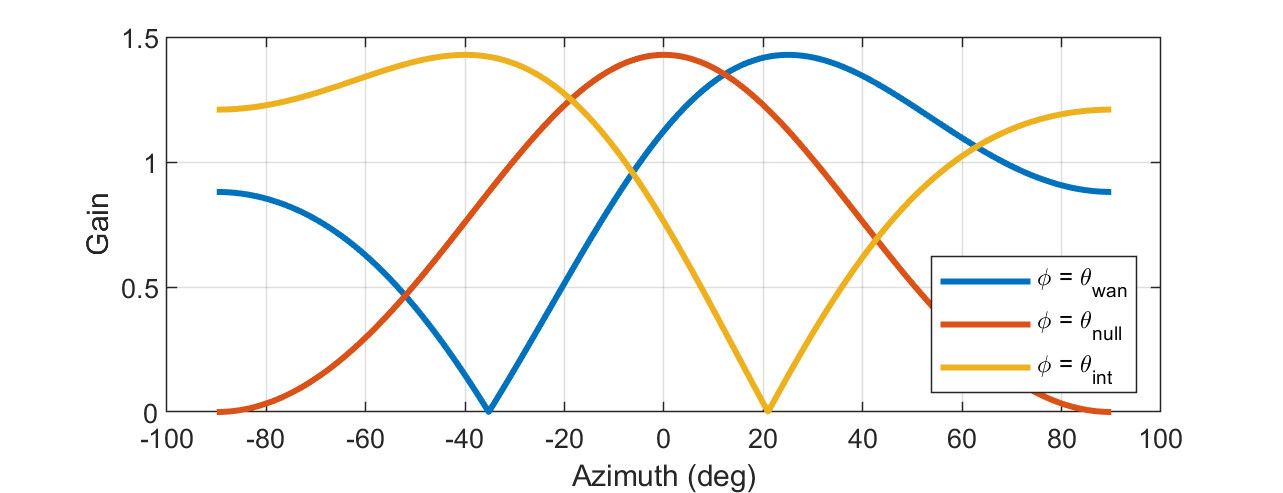
\includegraphics[width = 0.8\textwidth]{Figures/test_bf_rx_pattern.png}
    \caption{Theoretical radiation pattern for the beamformer at different steering angles.}
    \label{fig:test:bf:rx:pattern}
\end{figure}

\subsubsection{Magnitude and Phase} \label{test:bf:rx:mag}
The amplitude difference at different steering angles is given by the beamformer's radiation pattern, which is similar to a digital filter. The magnitude response of the beamformer is described in figure \ref{fig:test:bf:tx:pattern}, and the amplitude difference of $S_{wan}$ after the beamforming block at $\phi = \theta_{wan}$ and $\phi = \theta_{int}$ is shown in figure \ref{fig:fig:test:bf:rx:att}. The theoretical gain at $\phi = \theta_{wan}$ and $\phi = \theta_{int}$ is 1.41 and 0.147, respectively; hence, the gain ratio can be estimated and should be similar to the gain ratio of the real signals as shown in equation \ref{eq:test:bf:gain}.

\begin{equation}
\begin{gathered}
    \frac{|S_{wan}|_{\phi = \theta_{wan}}}{|S_{wan}|_{\phi = \theta_{int}}} \approx \frac{1.41}{0.147} = 9.59 \\
    \frac{|S_{wan}|_{\phi = \theta_{wan}}}{|S_{wan}|_{\phi = \theta_{int}}} = RMS(\frac{|S_{wan}(t)|_{\phi = \theta_{wan}}}{|S_{wan}(t)|_{\phi = \theta_{int}}}) = 10.12
    \label{eq:test:bf:gain}
\end{gathered}
\end{equation}
    
Similarly, the phase-shift of the beamformed signal can be validated by using the phase angle of the radiation pattern, instead of the magnitude as is often assumed. the "phase pattern" of the beamformer is shown in figure \ref{fig:test:bf:rx:phase}, and a validation for the beamformed signal's phase difference can be estimated by comparing the theoretical phase-difference using the phase pattern in figure \ref{fig:test:bf:rx:phase} and the actual phase difference of the real signals in figure \ref{fig:fig:test:bf:rx:att} as shown in equation \ref{eq:test:bf:phase} where $\mod$ represents the modulo operator. This equation outputs a phase angle comparable with the phase pattern in figure \ref{fig:test:bf:rx:phase}. 

\begin{equation}
\begin{gathered}
    \angle{S_{wan}(t)}_{\phi = \theta_{int}} - \angle{S_{wan}(t)}_{\phi = \theta_{wan}} \approx 43^\circ - 0^\circ \\
    \angle{S_{wan}(t)}_{\phi = \theta_{int}} - \angle{S_{wan}(t)}_{\phi = \theta_{wan}} = Mean(\angle{S_{wan}(t)}_{\phi = \theta_{int}} - \angle{S_{wan}(t)}_{\phi = \theta_{wan}}) -45^\circ \mod 45^\circ \\
    \angle{S_{wan}(t)}_{\phi = \theta_{int}} - \angle{S_{wan}(t)}_{\phi = \theta_{wan}} = Mod(133.5^\circ -45^\circ, 45^\circ) = 43.5^\circ
    \label{eq:test:bf:phase}
\end{gathered}
\end{equation}

The comparisons made with equations \ref{eq:test:bf:gain} and \ref{eq:test:bf:phase} show that the theoretical gain and phase of the beamformer is close to what $s_{wan}$ presents. This validation confirms that the beamformer behaves as the theory implies.

\begin{figure}[h]
    \centering
    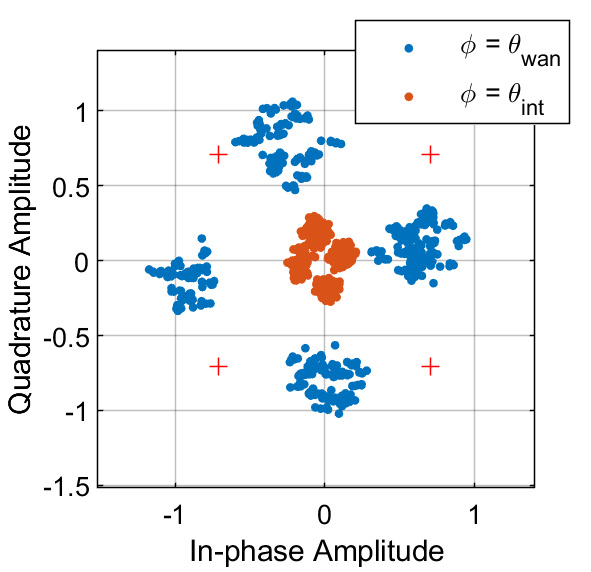
\includegraphics[width = 0.45\textwidth]{Figures/attenuation.png}
    \caption[Measured constellation diagram after the RX beamforming.]{Constellation diagram of $S_{wan}$ after the beamforming block  for the real implementation using a steering angle of $\phi = \theta_{wan}$ and $\phi = \theta_{int}$.}
    \label{fig:fig:test:bf:rx:att}
\end{figure}

\begin{figure}[h]
    \centering
    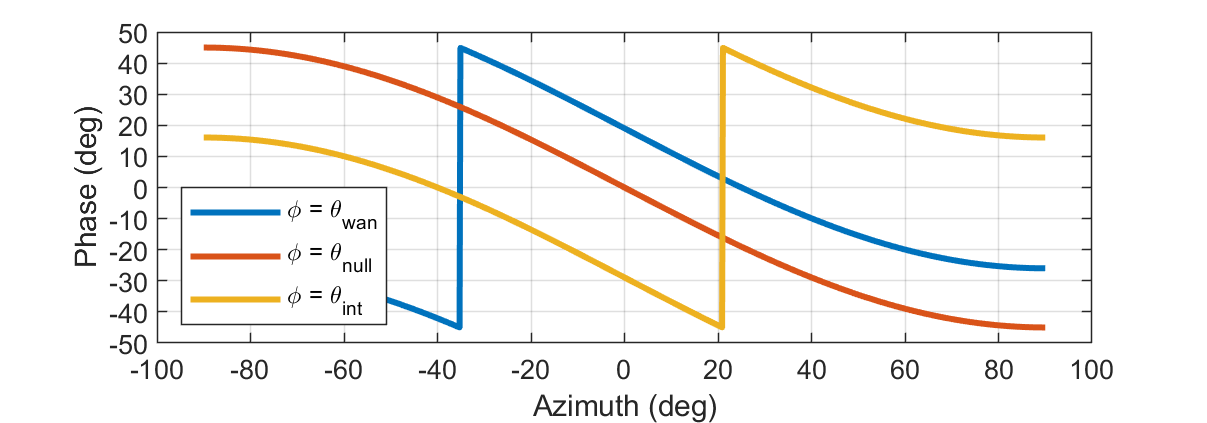
\includegraphics[width = 0.9\textwidth]{Figures/test_bf_rx_phase_pattern.png}
    \caption{Theoretical phase pattern for the beamformer at different steering angles.}
    \label{fig:test:bf:rx:phase}
\end{figure}

\newpage
\subsection{Direction of Arrival} \label{test:bf:rx:doa}
The validation test for the Direction of arrival calculation is done by using the beamforming equation in section \ref{back:bf:theoretical}. As previously stated, the incidence angle of a signal arriving at the RX antenna array causes a constant phase shift between the antenna elements. The complex weight $w_m$ contains the steering angle as its phase component; this component is described by equation \ref{eq:wn}. The phase offset in the baseband signal ($\alpha_{bb}$) is given by the phase component of the complex weight at element $m=1$; a reduced expression for the baseband phase angle is given by equation \ref{eq:test:bf:doa:phase:theo}, the output phase is given in both radians and degrees and assumes an optimal beamformer. In addition, the phase-shift of the received signals ($\hat{\alpha}_{bb}$) can be estimated by computing the mean phase difference between the received signals by each antenna element ($S_m$)  as shown in equation \ref{eq:test:bf:doa:phase:est}. 

\begin{equation}
    \alpha_{bb} = \angle{w_1^*} = -\pi \sin(\theta_{DOA}) = - 180 \sin(\theta_{DOA})
    \label{eq:test:bf:doa:phase:theo}
\end{equation}

\begin{equation}
    \hat{\alpha}_{bb} = Mean(\angle{S_0} - \angle{S_1})
    \label{eq:test:bf:doa:phase:est}
\end{equation}

The DOA estimation is validated using $S_{wan}$ from the previous section when sensed by both antenna elements in the SDR as $S_m$ for equation \ref{eq:test:bf:doa:phase:theo} and its computed DOA $\theta_{DOA} = \theta_{wan} = 25^\circ$ for equation \ref{eq:test:bf:doa:phase:theo}. The results of the previous computation output $\alpha_{bb} = -76.07^\circ$ and $\hat{\alpha}_{bb} = -78.66^\circ$; the similarity of both theoretical and estimated phase-differences validate the accuracy of the DOA estimator.

\begin{figure}[h]
    \centering
    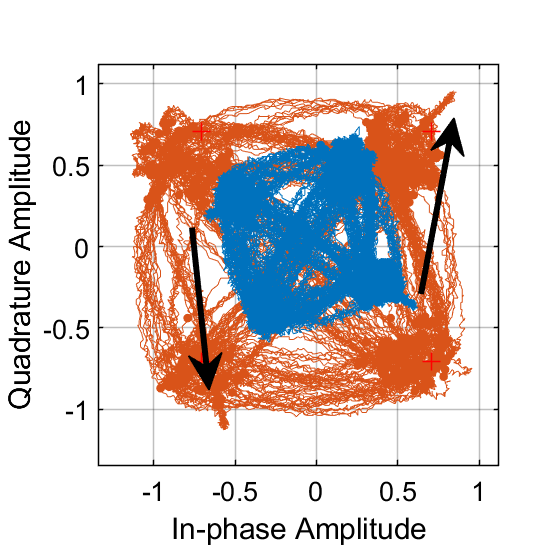
\includegraphics[width = 0.5\textwidth]{Figures/test_bf_doa_rx.png}
    \caption[Constellation diagram of the signal sensed by the RX antenna array.]{IQ signals for $S_{wan}$ after being sensed by each antenna element in the array from the real implementation.}
    \label{fig:test:bf:doa:rx}
\end{figure}

\newpage
\section{User Equipment Tracking} \label{test:ue}
 This last scenario consists of the BS tracking the UE as it moves in a large open area, as described in section \ref{met:sim}. The goal of this scenario is to test all the developed parts in a real-life situation. The metrics for this test are the BER and estimated DOA by the BS. These will be validated if the BS can estimate the UE location while maintaining a relatively low BER performance.
 
 The simulation and real runs differ, as briefly stated in section \ref{met:hil}. The simulation assumes a BS with two antenna arrays and a UE supporting beamforming at the receiving end, as stated in section \ref{met:sim}. However, the real implementation assumes both BS and UE have a single antenna array; transmitting and receiving, respectively. Overall, the main difference is that the steering angle of the TX beamformer in the BS is set as an input parameter, rather than being given by the signal coming from the UE. This decision was made because a real implementation of the model in figure \ref{fig:sim} would require three antenna arrays, and the available hardware only allows for two of these. Also, there is no way to run a Simulink model with two SDRs transmitting and receiving simultaneously using the available hardware; as many of the received samples are dropped due to timing issues. Hence, the real implementation only features a downlink system without any kind of feedback from the UE to the BS whatsoever. Although these assumptions may result in different results, the BER for both runs should have a consistent trend. 
 
 \subsection{Simulation} \label{test:ue:simulation}
 The simulation uses the model presented in figure \ref{fig:sim}, which contains all the blocks described in section \ref{met:sim}. The input parameters are the ones used in previous experiments such as tables \ref{tab:parameters:general}, \ref{tab:parameters:modulator} and \ref{tab:parameters:receiver}, and the remaining parameters are shown in table \ref{tab:parameters:sim}. The test consists of four runs, each one with a different combination of components (TX/RX beamformers and receiver); these are compared to the theoretical BER for QPSK. The DOA is only shown for the run that includes all the components.
 
 \begin{table}[h]
     \centering
     \begin{tabular}{c|c}
         Parameter & Value \\ \hline
         AWGN: Input Reference Power & 1 W \\ \hline
         UE: Movement period ($1/f_{UE}$) & 10 s \\
         UE: Maximum displacement angle ($DOD_{max}$) & $45^\circ$ \\
         UE: Azimuth ($\Azue$) & $15^\circ$ \\
     \end{tabular}
     \caption{Input parameters for the UE tracking simulation test.}
     \label{tab:parameters:sim}
 \end{table}

\begin{table}[h]
    \centering
    \begin{tabular}{c|c|c|c}
        Experiment Number & Modulator/Receiver & TX Beamformer & RX Beamformer \\ \hline
        (Ex) 1 & \checkmark & & \\
        (Ex) 2 & \checkmark & \checkmark &  \\
        (Ex) 3 & \checkmark & & \checkmark  \\
        (Ex) 4 & \checkmark & \checkmark & \checkmark
    \end{tabular}
    \caption{Component combination for each experiment in the UE tracking simulation test.}
    \label{tab:test:sim:ex}
\end{table}

The result in figure \ref{fig:test:sim:ber} show that experiment 1 have a worse BER than the theoretical, as stated in section \ref{test:mod_rec:rec} due to the timing error introduced by the symbol synchronisation. Experiments two and three have a similar impact in BER, as they both introduce the same gain improvement at their respective end, being this a factor of $\sqrt{2}$, as shown in figure \ref{fig:test:bf:tx:pattern} which also applies for RX beamformers. Introducing either a TX or RX beamformer to the system significantly improves the BER even while limited by the receiver. Finally, experiment four shows the best BER performance of them all, as the effect of both beamformers, is combined. 

\begin{figure}[h]
    \centering
    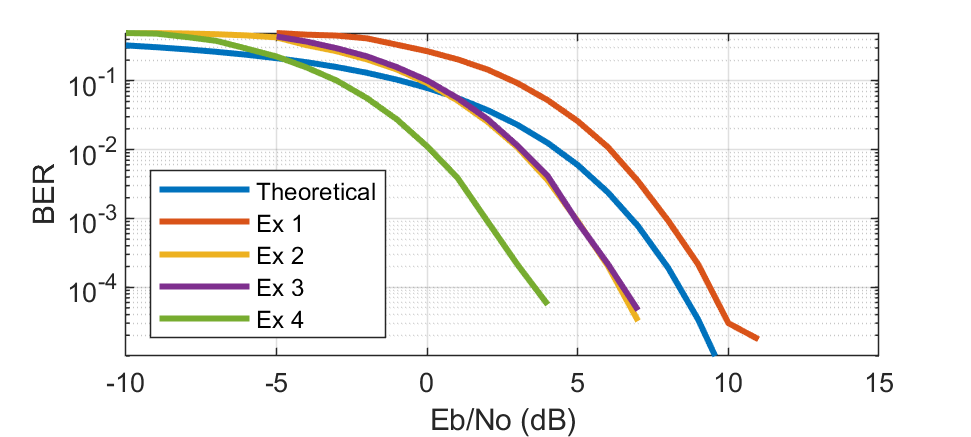
\includegraphics[width = 0.8\textwidth]{Figures/bf_ber_ebno.png}
    \caption{BER performance across experiments for the UE tracking simulation test.}
    \label{fig:test:sim:ber}
\end{figure}

The BER improvement introduced by both beamformers is also limited by the number of antennas in the array, as adding more antennas improves directivity, which increases the SNR at both ends. A few BER equivalents of experiment four are presented in figure \ref{fig:test:sim:ber_m} using $M = 2, 4, 8$.

\begin{figure}[h]
    \centering
    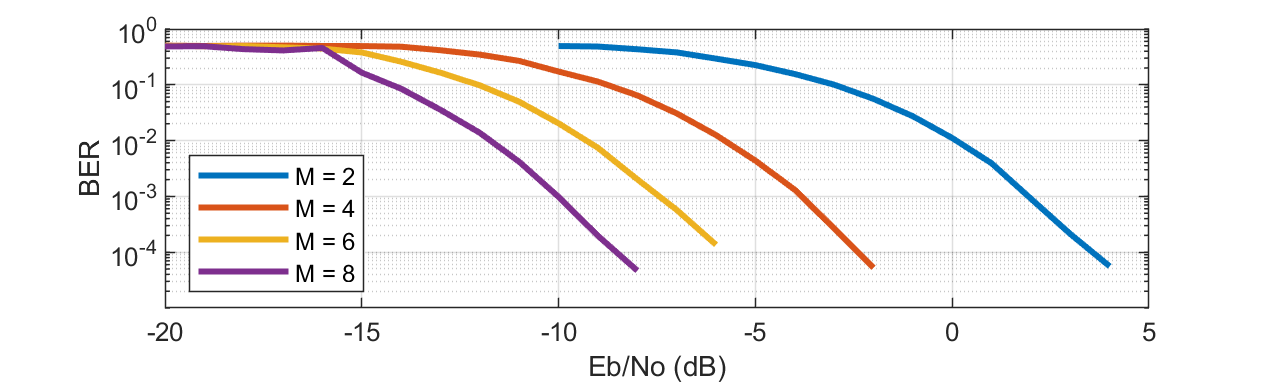
\includegraphics[width = \textwidth]{Figures/bf_ber_ebno_m.png}
    \caption{BER performance for systems with different antenna array elements for the UE tracking simulation test.}
    \label{fig:test:sim:ber_m}
\end{figure}

The second metric, the estimated DOA by the BS, is greatly affected by the channel's noise; hence, the steering angle may not be set to the actual location of the UE. The beam of a two-element array is not very narrow, so the estimation error does not affect the BER as much as in an array with many antenna elements. Figure \ref{fig:test:sim:dod} shows the measured DOD across simulation time, which proves that lower SNRs add noise to the estimation. Finally, even with low SNR conditions and poor angle estimation, the BER performance shows that a communication link can be established.

\begin{figure}[h]
    \centering
    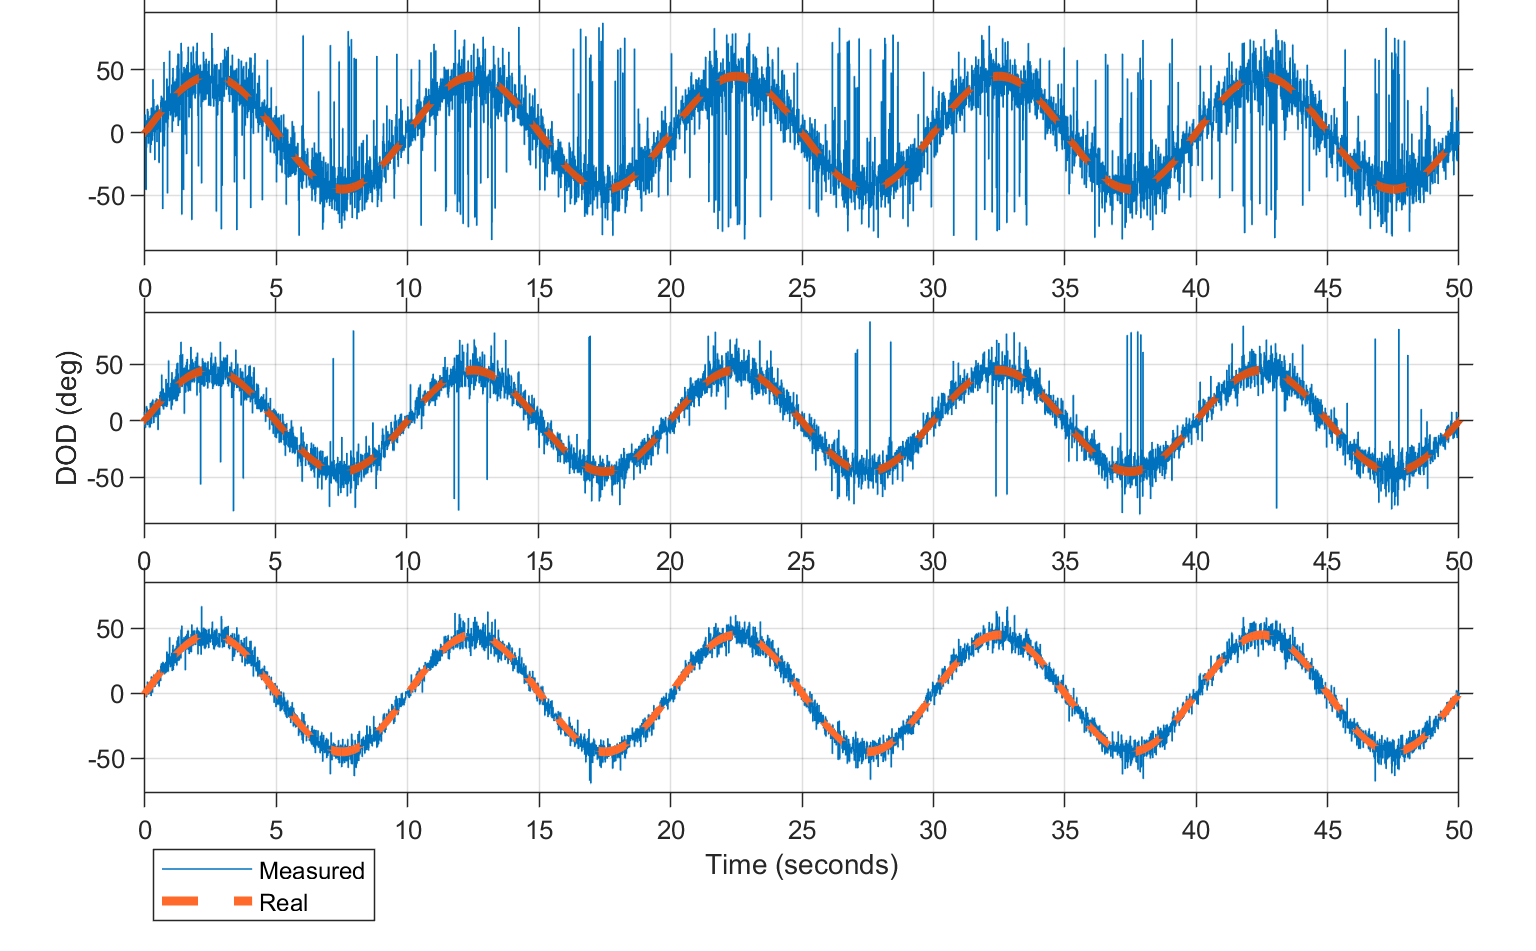
\includegraphics[width = \textwidth]{Figures/test_sim_dod_snr.png}
    \caption[Measured DOD for the UE tracking simulation test.]{Estimated DOD using Eb/No = -2 dB, 0 dB and 2 dB for the UE tracking simulation test.}
    \label{fig:test:sim:dod}
\end{figure}

\subsection{Real Implementation} \label{test:ue:real}
As previously mentioned, the real implementation of the UE tracking scenario uses two antenna arrays, one representing the transmitting end of the BS while the other represents the receiving end of the UE. Since the two antenna arrays are joined together to the SDR with one metre SMA cables, the moving array cannot move freely around the other, making the test scenario more challenging. In the end, the test scenario consisted of the BS sweeping the DOD by using the same sinusoidal movement pattern as the one described in section \ref{fig:sl:movement}, maximum DOD ($DOD_{max}$) and movement frequency ($f_{UE}$). The receiving end of the implementation must estimate the DOA of the received signal and steer the RX beamformer's main beam towards the incoming signal. 

The Simulink model used for this test is shown in figure \ref{fig:hil_demo}, only replacing the TX steering angle by the DOD function in equation \ref{eq:DOD} represented in figure \ref{fig:sl:movement}. The test took place in four different environments: side-by-side, facing each other, perpendicular and indoors. These scenarios vary in different ways, as the location and orientation of the antenna arrays and the resulting multipath propagation effect of the received signal affect the estimated DOA. 

\begin{figure}[h]
    \centering
    \begin{subfigure}{0.45\textwidth}
        \centering
        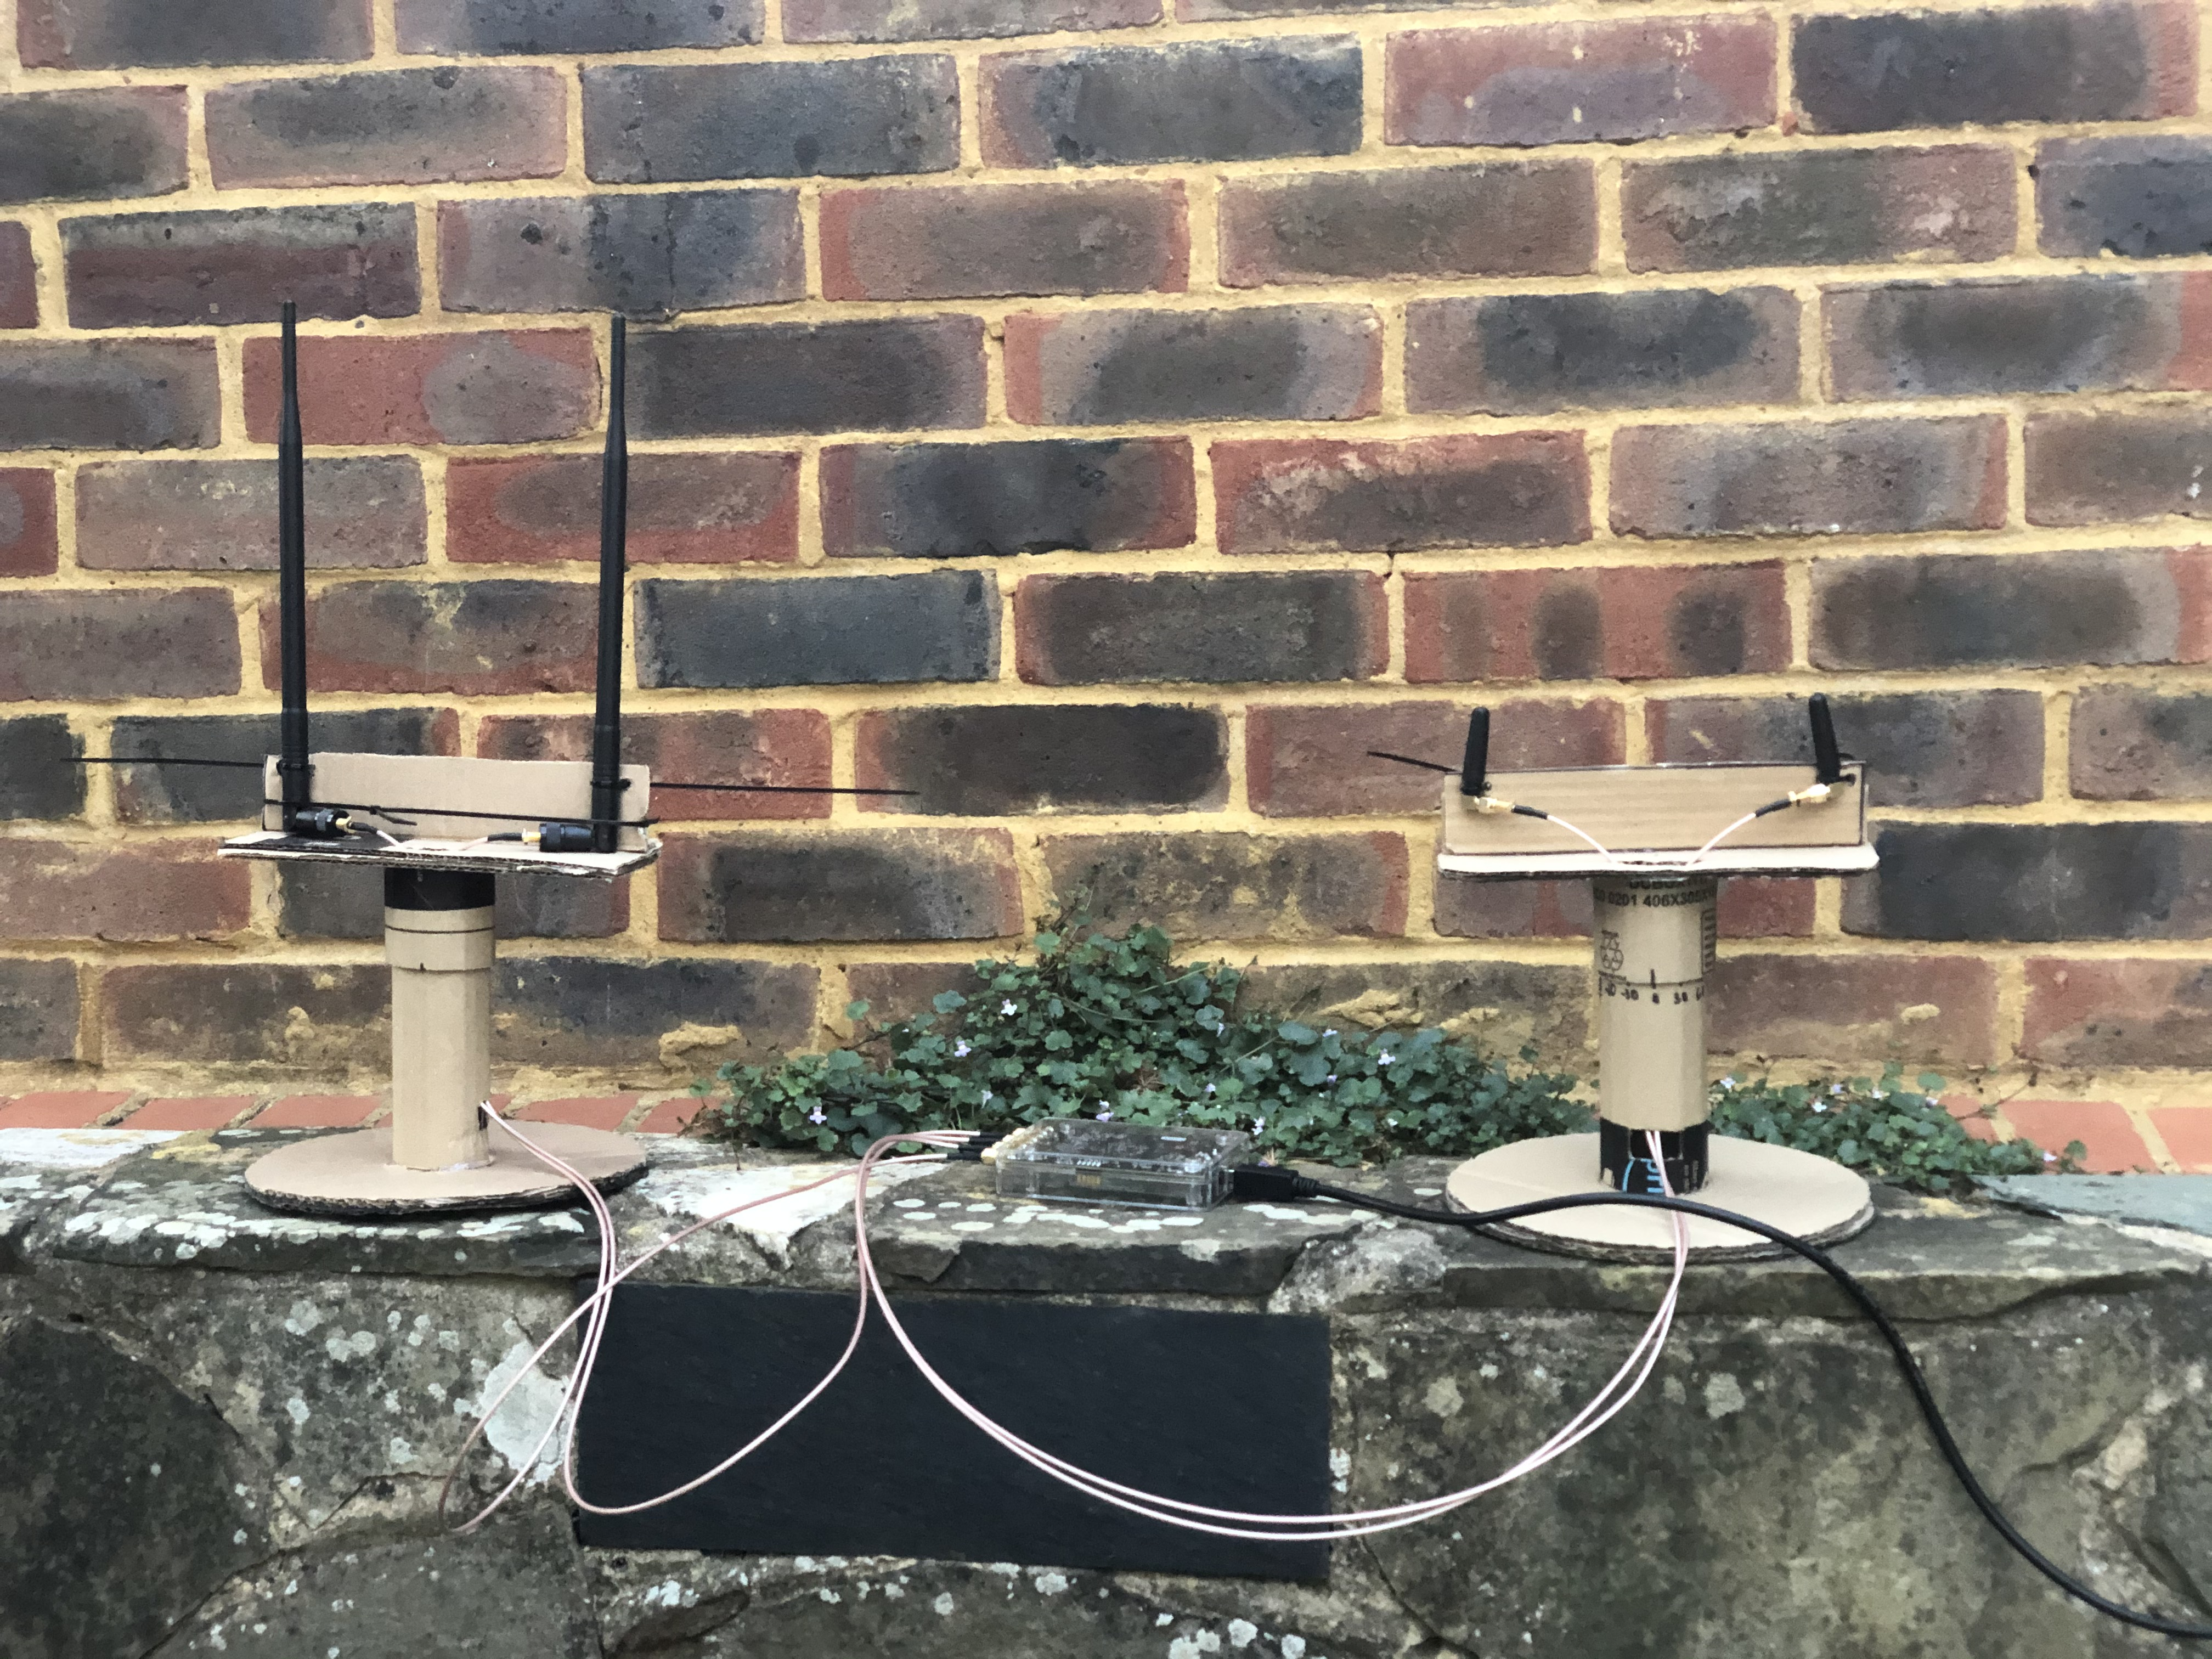
\includegraphics[width = \textwidth]{Figures/test_ue_side_by_side.jpg}
        \caption{Side-by-side}
        \label{fig:test:ue:env:sbs}
    \end{subfigure}
    \hfill
    \begin{subfigure}{0.45\textwidth}
        \centering
        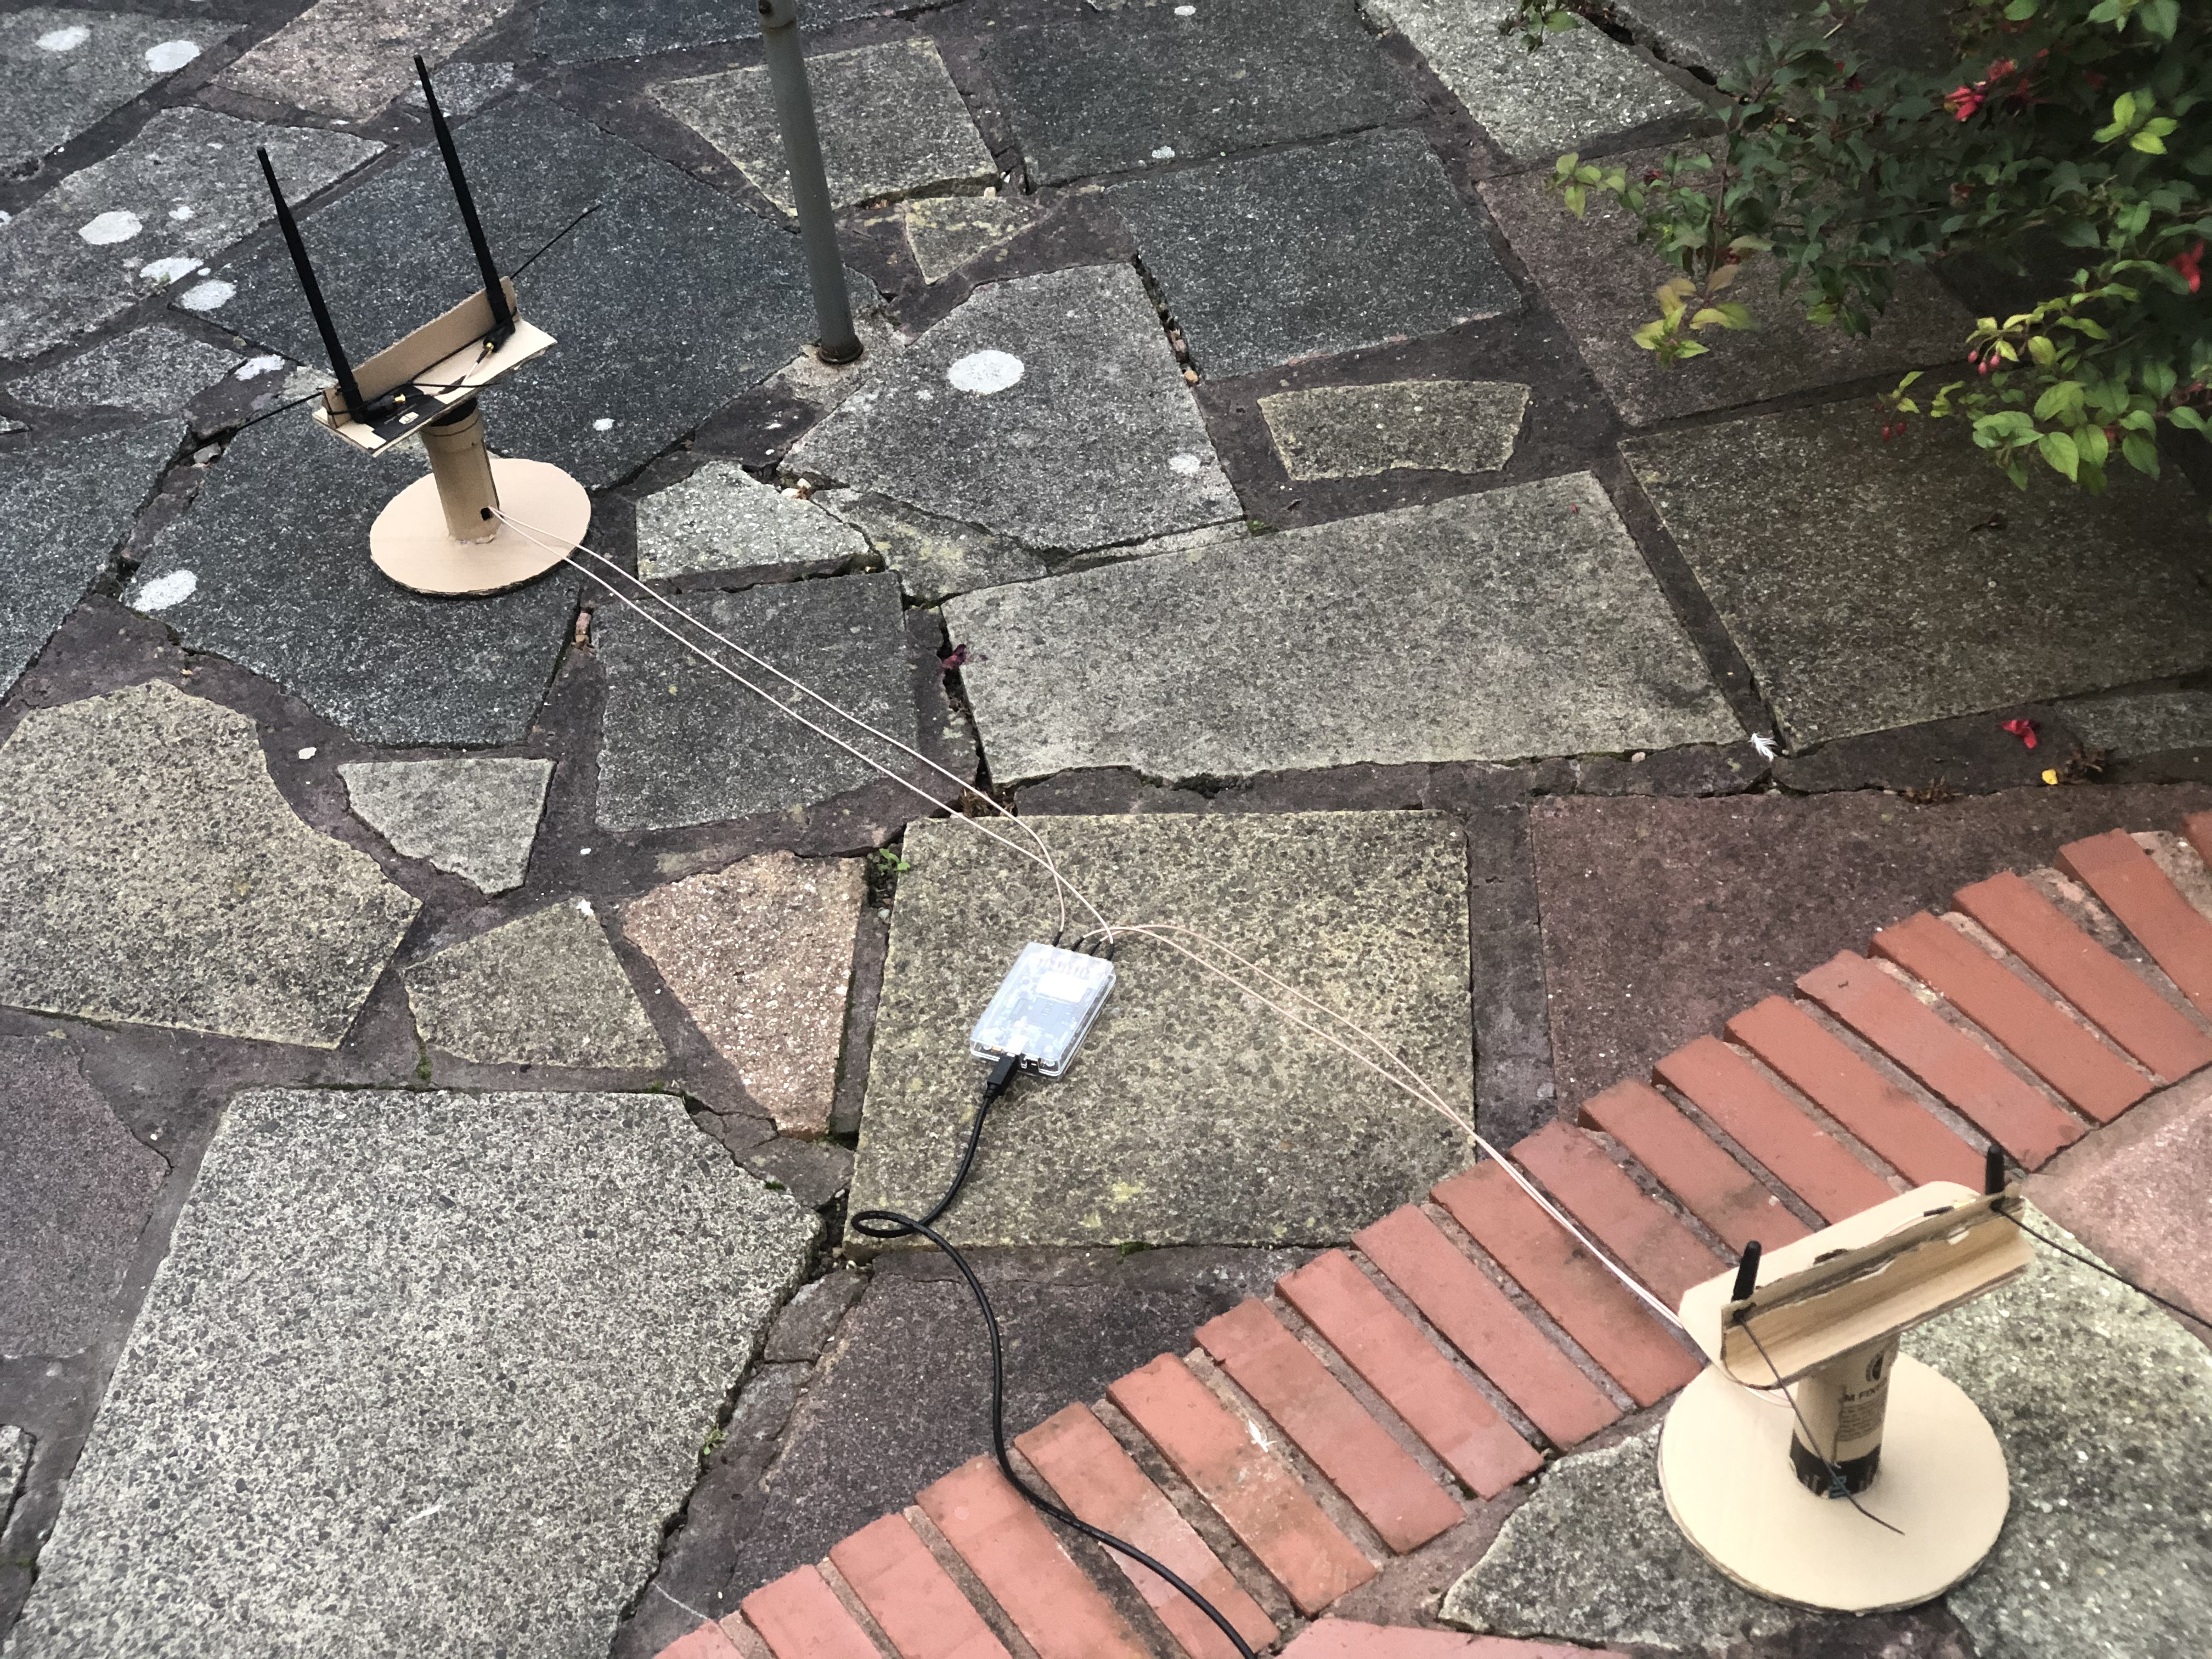
\includegraphics[width = \textwidth]{Figures/test_ue_facing.jpg}
        \caption{Facing each other}
        \label{fig:test:ue:env:fac}
    \end{subfigure}
    
    \begin{subfigure}{0.45\textwidth}
        \centering
        \includegraphics[width = \textwidth]{Figures/test_ue_perpendicular.jpg}
        \caption{Perpendicular}
        \label{fig:test:ue:env:perp}
    \end{subfigure}
    \hfill
    \begin{subfigure}{0.45\textwidth}
        \centering
        \includegraphics[width = \textwidth]{Figures/test_ue_indoors.jpg}
        \caption{Indoors}
        \label{fig:test:ue:env:ind}
    \end{subfigure}
    \caption{Real test environments for the UE tracking test}
    \label{fig:test:ue:env}
\end{figure}

The system parameters are consistent for all four environments and, similar to the simulation section, uses the system parameters of the previous tests in addition to $DOD_{max} = 30^\circ$ and $1/f_{UE} = 10$ seconds. The test runs are 30 seconds long to capture several periods of the steering pattern to validate its repeatability. 

Each environment in figure \ref{fig:test:ue:env} has different surfaces in which the transmitted signal can bounce and propagate. The side-by-side environment shown in figure \ref{fig:test:ue:env:sbs} consists of the two antenna elements placed within a parallel axis near a wall; the $x$ axis of both arrays point towards a glass door in which the signals can bounce quickly. The environment in figure \ref{fig:test:ue:env:fac} show both arrays facing each other at a close distance; this distance might not be enough for the signal to propagate properly by the beamformer. The perpendicular environment in figure \ref{fig:test:ue:env:perp} show both arrays placed, making both $x$ axes perpendicular; some low-height walls surround the arrays. Finally, both arrays are placed indoor as shown in figure \ref{fig:test:ue:env:ind}; this scenario is expected to be significantly influenced by multipath propagation, as the walls and ceiling make the signal bounce greatly.

The results for these tests are shown in table \ref{tab:test:ue:real:ber} and figures \ref{fig:test:ue:real:err} and \ref{fig:test:ue:doa}. Table \ref{tab:test:ue:real:ber} proves that the communication link for every test environment was stable as the BER is relatively low. Figure \ref{fig:test:ue:real:err} show the number of error of the communications system across time, and it can be noticed that the errors mostly come from the first second, as the carrier synchronisation is still reaching its steady-state. After reaching the steady-state, only few errors are introduced, and the error number remains fairly consistent across time. Most environments showed this behaviour, excepting the one in which both arrays are facing each other, as it has the most error before the steady-state and there is a considerable increase long after the fact. The close distance between arrays might cause this behaviour. However, the indoor environment showed the best BER performance, as the steady-state errors are considerably lower than the parallel and side-by-side environments. This performance may be the result of the multipath propagation of the room.

\begin{table}[h]
    \centering
    \begin{tabular}{c|c}
        Environment & BER \\ \hline
        Side-by-side & 0.0025 \\
        Facing each other & 0.0079 \\
        Perpendicular & 0.0028 \\
        Indoor & 0.0016
    \end{tabular}
    \caption{Resulting BER for the UE tracking test}
    \label{tab:test:ue:real:ber}
\end{table}

\begin{figure}[h]
    \centering
    \includegraphics[width = \textwidth]{Figures/test_ue_errors.png}
    \caption{Errors across time for each environment in the UE tracking test.}
    \label{fig:test:ue:real:err}
\end{figure}

Figure \ref{fig:test:ue:doa} show the estimated DOA given a time-variant DOD for all four testing environments. Since the received signal by the RX antenna array is greatly affected by multipath and other impairments, the estimated DOA is not supposed to match the DOD; only a sinusoidal shaped signal is expected as this is the shape of the DOD. The objective of these tests is to prove that the estimated DOA by the receiver end is affected by the input DOD. The side-by-side environment profile in figure \ref{fig:test:ue:doa:sbs} shows a DOA profile close to being purely sinusoidal, which is obtained across all three periods in the test run time. The environment with both arrays facing each other in figure \ref{fig:test:ue:doa:fac} shows some discontinuities, which may be caused by the $\pm 90$ range constraint of the estimation algorithm. Considering the lower peaks are a product of this constraint, then the DOA profile would look like a rectified sinusoid, with little to no impact from the negative side of the DOD sinusoid. Figure \ref{fig:test:ue:doa:perp} shows a sinusoidal pattern with reduced amplitude and a large offset, caused by the already high incidence angle between antenna arrays. Lastly, figure \ref{fig:test:ue:doa:ind} shows a saturated sinusoid in the indoor environment which may be caused by the walls and the objects inside the room.

\begin{figure}[h]
    \centering
    \begin{subfigure}{0.45\textwidth}
        \centering
        \includegraphics[width = \textwidth]{Figures/test_doa_sbs.png}
        \caption{Side-by-side}
        \label{fig:test:ue:doa:sbs}
    \end{subfigure}
    \hfill
    \begin{subfigure}{0.45\textwidth}
        \centering
        \includegraphics[width = \textwidth]{Figures/test_doa_fac.png}
        \caption{Facing each other}
        \label{fig:test:ue:doa:fac}
    \end{subfigure}
    
    \begin{subfigure}{0.45\textwidth}
        \centering
        \includegraphics[width = \textwidth]{Figures/test_doa_par.png}
        \caption{Perpendicular}
        \label{fig:test:ue:doa:perp}
    \end{subfigure}
    \hfill
    \begin{subfigure}{0.45\textwidth}
        \centering
        \includegraphics[width = \textwidth]{Figures/test_doa_ind.png}
        \caption{Indoors}
        \label{fig:test:ue:doa:ind}
    \end{subfigure}
    \caption[DOA measurements for the UE tracking tests.]{Estimated DOA (orange) from the received signals and the input DOD (green, dotted) for the real UE tracking test.}
    \label{fig:test:ue:doa}
\end{figure}

As expected, the estimated DOA seems to be affected by the input DOD, but in the case of figures \ref{fig:test:ue:doa:fac} and \ref{fig:test:ue:doa:ind}, these show some non-linear properties in the form of rectification and saturation, respectively. 

Overall, the results were as expected, as the communication link was maintained while varying the DOD, and it was proven that the DOD affected the estimated DOA without moving the antenna arrays.

\chapter{Conclusions} \label{conc}
The work done in the previous chapters show that both TX and RX digital beamformers can be implemented in low-cost SDR units just by knowing the hardware requirements and applying the algorithm in software. However, these requirements limit the hardware that can be used to a smaller sub-set, which is still more expensive than the commonly available RTL-SDR, but still a lot cheaper than the high-end brands as Ettus Research. 

Also, a contribution to the SDR community was made, as the MATLAB interface for the BladeRF developed in section \ref{met:int} is meant to be continued to fix some existing issues and then submitted into Nuand's repository for it to be available in the official repository if accepted by the manufacturer.

Chapter \ref{test} proved that the work done in this project resulted in a beamforming system, but also required an enormous amount of effort and research to use SDRs and establish a working communications system. The proposed receiver scheme resented in section \ref{met:sim:mod:rec} could be the topic for another project, as there are many subsystems to enhance data throughput or error performance. The used receiver scheme, although it has its share of complexity, does not feature other techniques as MIMO or error detection, which can significantly improve its performance.

The final test scenario in section \ref{test:ue:real} was constrained due to limited hardware, but its results show that a proof of concept was achieved, which is the primary goal of this project. However, the similarity of the simulations to the real results (in terms of error rate) may indicate that the same trend found in the results of section \ref{test:ue:simulation} could be found if the real implementation was done with the same elements as the simulation.

The developed system's performance is satisfactory, as it roughly matched the theoretical responses and the simulation results. As of the objectives of section \ref{intro:obj}, all the primary objectives were satisfied, as a the prototype uses the HIL design paradigm, the software is flexible and capable of handling different TX and RX beamformers based on the contents of chapter \ref{back}. The system is capable of tracking signals using the DOA estimator while maintaining an acceptable error performance. Also, every secondary goal was achieved, as the prototype is scalable by using multiple SDR units and the system simulation is accurate and contains the same blocks as the prototype. However, many improvements can still be introduced. Overall, the project is considered a success and a great topic for a follow-up project. 

\section{Future Work} \label{conc:future}
Many things can be done to follow the work presented for this project. The nearest thing to do would be to increase the number of antenna elements by combining two or more BladeRF units; the software interface for the BladeRF would have to be updated to feature multi-IC synchronisation, and the Simulink system-object must consider the data coming from the multiple devices and align it. Other than that, the simulation and remaining subsystems already support a variable number of antennas, as shown in figure \ref{fig:test:sim:ber_m}. A different antenna array geometry can be implemented in order to support both azimuth and elevation steering.

Once many SDRs can be implemented simultaneously, the antenna array may be split to obtain multiple independent beams. This feature is useful if a Multiple Access scheme using beamforming is intended. 

This same algorithm may be implemented using the GNU Radio Companion software, this to benefit from its open-source code and to combine it with different applications using its Python framework.

As a more complex flow-up, hybrid beamforming may be implemented in order to get sub-beams inside the analogue beam. This upgrade may require to modify or bypass the RF section of the SDR in order to attach its output to the analogue beamformer.

\appendix
\chapter{Repository} \label{appendix}
The Simulink model, MATLAB scripts and CAD files are available in the following git repository. The directory structure and files are described in the README section.

\url{https://github.com/JoseAmador95/UoS_Beamforming.git}


\bibliographystyle{ieeetr}
\bibliography{references.bib}

\end{document}
